\documentclass[]{article}
\usepackage{proceed2e}

% Set the typeface to Times Roman
\usepackage{times}


% For figures
\usepackage{graphicx} % more modern
%\usepackage{epsfig} % less modern
%\usepackage{subcaption} 
%usepackage[numers]{natbib}
% For citations
%\usepackage[numbers]{natbib}

% For algorithms
%\usepackage{algorithm}
%\usepackage{algorithmic}

% As of 2011, we use the hyperref package to produce hyperlinks in the
% resulting PDF.  If this breaks your system, please commend out the
% following usepackage line and replace \usepackage{icml2014} with
% \usepackage[nohyperref]{icml2014} above.
%\usepackage{hyperref}
% Packages hyperref and algorithmic misbehave sometimes.  We can fix
% this with the following command.
%\newcommand{\theHalgorithm}{\arabic{algorithm}}

% Employ the following version of the ``usepackage'' statement for
% submitting the draft version of the paper for review.  This will set
% the note in the first column to ``Under review.  Do not distribute.''
\usepackage{bm}
\usepackage{amsmath}
\usepackage[numbers]{natbib}
%\usepackage{array}
%\usepackage{nips_style} 
%\usepackage{sidecap}
%\usepackage[export]{adjustbox}
%\newcommand{\lp}{\left(}
\newcommand{\rp}{\right)}
\newcommand{\lb}{\left[}
\newcommand{\rb}{\right]}

\newcommand{\N}{N}
\newcommand{\cind}{t}
\newcommand{\pind}{\star}

\newcommand{\xvec}{{\bf x}}
%\newcommand{\xp}{\xvec^{\pind}}
%\newcommand{\xt}{\xvec_{\cind}}
\newcommand{\s}{\sigma}
\newcommand{\muz}{\mu_z}
\newcommand{\muc}{\mu_c}
\newcommand{\mup}{\mu_{\pind}}
\newcommand{\mut}{\mu_{\cind}}
\newcommand{\mutrue}{\mu_{\tau}}
\newcommand{\sz}{\sigma_z}
\newcommand{\ahat}{\hat{\alpha}}
\newcommand{\pitilde}{\tilde{\pi}}
\newcommand{\K}{{\bf K}}
\newcommand{\kv}{{\bf k}}
\newcommand{\kk}{k}

\newcommand{\fx}{f\lp \xvec \rp}
\newcommand{\fxt}{f\lp \xt \rp}
\newcommand{\fxp}{f\lp \xp \rp}

\newcommand{\mx}{m\lp \xvec \rp}
\newcommand{\m}{m}
\newcommand{\z}{z}

\newcommand{\error}{\xi}
\newcommand{\acceptance}{\alpha}

\newcommand{\scale}{s}
\newcommand{\zs}{\z_{\scale}}

\newcommand{\accmon}{\alpha}
\newcommand{\decay}{\gamma}

\newcommand{\disc}{\rho}
\newcommand{\eps}{\epsilon}
\newcommand{\Keps}{K_{\eps}}
\newcommand{\Y}{Y}
\newcommand{\X}{{\bf X}}
\newcommand{\xs}{x}
\newcommand{\x}{{\bf x}}
\newcommand{\y}{{\bf y}}
\newcommand{\ys}{\y^{(s)}}
%\newcommand{\yone}{\y^{(1)}}
%\newcommand{\yS}{\y^{(S)}}
\newcommand{\yp}{\y^{\prime}}
\newcommand{\yps}{\y^{\prime(s)}}
%\newcommand{\ypone}{\y^{\prime(1)}}
\newcommand{\ypS}{\y^{\prime(S)}}
\newcommand{\yjs}{y_j^{(s)}}
\newcommand{\yone}{\y^{(1)}}
\newcommand{\yS}{\y^{(S)}}
\newcommand{\ypone}{\y^{'(1)}}
\newcommand{\xp}{\x^{\prime}}
\newcommand{\xps}{\x^{\prime(s)}}
\newcommand{\xpone}{\x^{\prime(1)}}
\newcommand{\Xtheta}{\X_{\theta}}
\newcommand{\mutheta}{{\bm \mu}_{\thetav}}
\newcommand{\vtheta}{\sigma_{\theta}^2}

\newcommand{\thetap}{\theta^{\prime}}
\newcommand{\Xthetap}{\X_{\thetap}}
\newcommand{\muthetap}{{\bm \mu}_{\thetapv}}
\newcommand{\vthetap}{\sigma_{\thetap}^2}
\newcommand{\sthetap}{\sigma_{\thetap}}
\newcommand{\stheta}{\sigma_{\theta}}

\newcommand{\xtheta}{\x|\theta}
\newcommand{\xthetap}{\x|\theta^{\prime}}
\newcommand{\w}{{\bf w}}
\newcommand{\thetamat}{ {\bm \Theta}}
\newcommand{\thetav}{{\bm \theta}}
\newcommand{\thetapv}{{\bm \theta^{\prime}}}
\newcommand{\thetavp}{\thetapv}
\newcommand{\muhattheta}{\hat{{\bm \mu}}_{\thetav}}
\newcommand{\sigmahattheta}{\hat{\sigma}^2_{x|\thetav}}
\newcommand{\Sigmahattheta}{\hat{{\bm \Sigma}}_{\thetav}}
\newcommand{\muhatthetap}{\hat{{\bm \mu}}_{\thetapv}}
\newcommand{\sigmahatthetap}{\hat{\sigma}^2_{x|\thetapv}}
\newcommand{\Sigmahatthetap}{\hat{{\bm \Sigma}}_{\thetapv}}
\newcommand{\Sigmatheta}{{\bm \Sigma}_{\thetav}}
\newcommand{\bfSigmap}{{\bm \Sigma}_{\thetapv}}
\newcommand{\bfSigma}{{\bm \Sigma}_{\thetav}}
\newcommand{\p}{\pi}
\newcommand{\eye}{{\bm I}}


\newcommand{\muhatthetaj}{\hat{\mu}_{j}}
\newcommand{\sigmahatthetaj}{\hat{\sigma}^2_{j}}
%\newcommand{\sigmahattheta}{\hat{\sigma}^2_{x|\thetav}}

\newcommand{\muthetapm}{{\bm \mu}^{(m)}_{\thetapv}}
\newcommand{\muthetam}{{\bm \mu}^{(m)}_{\thetav}}
\newcommand{\Sigmahatthetathetap}{\hat{{\bm \Sigma}}_{\thetav\thetapv}}
\newcommand{\Sigmahatthetaptheta}{\hat{{\bm \Sigma}}_{\thetapv\thetav}}
\newcommand{\Sigmathetatheta}{{{\bm \Sigma}}_{\thetav\thetav}}

\newcommand{\Kthetatheta}{ {\bm K}_{\thetav\thetav}}
\newcommand{\Kthetapthetap}{ {\bm K}_{\thetapv\thetapv}}
\newcommand{\Kthetathetap}{ {\bm K}_{\thetav\thetapv}}
\newcommand{\Kthetaptheta}{ {\bm K}_{\thetapv\thetav}}
\newcommand{\alpham}{\alpha^{(m)}}

\newcommand{\muthetapj}{\mu_{\thetapv j}}
\newcommand{\muthetaj}{\mu_{\thetav j}}
\newcommand{\muthetapjbar}{{\bar \mu}_{\thetapv j}}
\newcommand{\muthetajbar}{{\bar \mu}_{\thetav j}}

\newcommand{\muthetapmj}{\mu^{(m)}_{\thetapv j}}
\newcommand{\muthetamj}{\mu^{(m)}_{\thetav j}}

\newcommand{\sigmasqthetap}{\sigma^2_{\thetapv j}}
\newcommand{\sigmasqtheta}{\sigma^2_{\thetav j}}
\newcommand{\sigmathetathetap}{\sigma_{\thetav\thetapv j}}
\newcommand{\sigmathetaptheta}{\sigma_{\thetapv\thetav j}}
\newcommand{\thetan}{{\bm \theta}_n}
\newcommand{\xn}{{\bm \x}_n}
\newcommand{\yj}{y_j}
\newcommand{\yji}{y_j^{(n)}}
\newcommand{\kthetapN}{{\bm k}_{\thetapv \thetamat j}}
\newcommand{\kthetaN}{{\bm k}_{\thetav \thetamat j}}
\newcommand{\kthetapthetap}{k_{\thetapv \thetapv j}}
\newcommand{\kthetatheta}{k_{\thetav \thetav j}}
\newcommand{\kthetaptheta}{k_{\thetapv \thetav j}}
\newcommand{\kthetathetap}{k_{\thetav \thetapv j}}
\newcommand{\KNN}{{\bm K}_{\thetamat\thetamat j}}
\newcommand{\errorcond}{\mathcal{E}_u(\alpha)}
\newcommand{\erroruncond}{\mathcal{E}(\alpha)}
\newcommand{\ymu}{\muhattheta}
\newcommand{\simsim}{\overset{\simulator}{\sim}}
\newcommand{\ystar}{\y^{\star}}
\newcommand{\thetastar}{\thetav^{\star}}
\newcommand{\thetavi}{\thetav^{(n)}}
%\newcommand{\yj}{y_j}
\newcommand{\ystarj}{\yj^{\star}}
\newcommand{\ystarjup}{\yj^{\star b}}
\newcommand{\ystarjlow}{\yj^{\star a}}
\newcommand{\ymc}{\y^{(s)}}
\newcommand{\epsvec}{ {\bm \eps}}
\newcommand{\epsj}{\eps_j}
\newcommand{\F}{F}
\newcommand{\Heavy}{H}
\newcommand{\kernelwidth}{h}
\DeclareMathOperator\simulator{sim}
\DeclareMathOperator\erf{erf}
\DeclareMathOperator\mean{mean}
\DeclareMathOperator\median{median}
\DeclareMathOperator\mode{mode}
\DeclareMathOperator*{\argmax}{arg\,max}
\DeclareMathOperator\expdist{Exp}
\newcommand{\params}{p}
\newcommand{\E}{E}
\newcommand{\yemaj}{\yj^{\textsc{ema}}}
\newcommand{\yema}{\y^{\textsc{ema}}}
\newcommand{\epsemaj}{\epsj^{\textsc{ema}}}
\newcommand{\epsema}{\epsvec^{\textsc{ema}}}
\newcommand{\epsmin}{\epsvec^{\textsc{min}}}
\newcommand{\epsminj}{\epsj^{\textsc{min}}}
\newcommand{\epsquantile}{\beta}
\newcommand{\geom}{{\bf g}}

\newcommand{\bx}{\xvec}

\newcommand{\gradv}{ {\bm g }}
\newcommand{\gradvest}{ \hat{\gradv}}
\newcommand{\gradestimate}[2]{\hat{g}_{#1}\lp#2\rp}
\newcommand{\gradestimaterepeat}[3]{\hat{g}^{#3}_{#1}\lp#2\rp}
\newcommand{\feval}[2]{y_{#1}^{#2}}
\newcommand{\cstep}[2]{c_{#1#2}}
\newcommand{\cstepconst}[1]{c_{#1}}
\newcommand{\dstep}[2]{\Delta_{#1#2}}
\newcommand{\dstepconst}[1]{\Delta_{#1}}
\newcommand{\loglik}[1]{L\lp#1\rp}

\newcommand{\gmom}{g_m}
\newcommand{\gsquare}{v_m}
\newcommand{\rhov}{ {\bm \rho}}
\newcommand{\zerov}{ {\bm 0}}
\newcommand{\omegav}{ {\bm \omega}}
\newcommand{\omegas}{ \omega_s}
\newcommand{\varv}{ {\bm V}}
\newcommand{\Bv}{ {\bm B}}
\newcommand{\Cv}{ {\bm C}}
\newcommand{\yi}{\y_i}
\newcommand{\Deltav}{{\bm \Delta}}
\newcommand{\Deltavd}{\Deltav_d}
\newcommand{\Deltavr}{\Deltav_r}
\newcommand{\deltad}{\delta_d}
\newcommand{\thetavd}{\thetav_d}
\newcommand{\thetavplus}{\thetav^{+}}
\newcommand{\thetavminus}{\thetav^{-}}
\newcommand{\thetavplusd}{\thetav^{+}_d}
\newcommand{\thetavminusd}{\thetav^{-}_d}
\newcommand{\thetavpmd}{\thetav^{\pm}_d}
\newcommand{\thetavpm}{\thetav^{\pm}}
\newcommand{\xpluss}{\x^{+}_s}
\newcommand{\xminuss}{\x^{-}_s}
\newcommand{\xplussd}{\x^{+}_{sd}}
\newcommand{\xminussd}{\x^{-}_{sd}}
\newcommand{\xpmd}{\x^{\pm}_{d}}
\newcommand{\lleps}{\mathcal{L}_{\epsvec}}
\newcommand{\dtheta}{d_{\thetav}}

% For algorithms
\usepackage{algorithm}
\usepackage{algorithmic}

% As of 2011, we use the hyperref package to produce hyperlinks in the
% resulting PDF.  If this breaks your system, please commend out the
% following usepackage line and replace \usepackage{icml2014} with
% \usepackage[nohyperref]{icml2014} above.
%\usepackage{hyperref}
% Packages hyperref and algorithmic misbehave sometimes.  We can fix
% this with the following command.
%\newcommand{\theHalgorithm}{\arabic{algorithm}}

% Leave date blank
\date{}

\pagestyle{myheadings}
%\usepackage{sidecap}
%\usepackage[export]{adjustbox}

%\newcommand{\theHalgorithm}{\arabic{algorithm}}

\newcommand{\fix}{\marginpar{FIX}}
\newcommand{\new}{\marginpar{NEW}}

\newcommand{\lp}{\left(}
\newcommand{\rp}{\right)}
\newcommand{\lb}{\left[}
\newcommand{\rb}{\right]}

\newcommand{\N}{N}
\newcommand{\cind}{t}
\newcommand{\pind}{\star}

\newcommand{\xvec}{{\bf x}}
%\newcommand{\xp}{\xvec^{\pind}}
%\newcommand{\xt}{\xvec_{\cind}}
\newcommand{\s}{\sigma}
\newcommand{\muz}{\mu_z}
\newcommand{\muc}{\mu_c}
\newcommand{\mup}{\mu_{\pind}}
\newcommand{\mut}{\mu_{\cind}}
\newcommand{\mutrue}{\mu_{\tau}}
\newcommand{\sz}{\sigma_z}
\newcommand{\ahat}{\hat{\alpha}}
\newcommand{\pitilde}{\tilde{\pi}}
\newcommand{\K}{{\bf K}}
\newcommand{\kv}{{\bf k}}
\newcommand{\kk}{k}

\newcommand{\fx}{f\lp \xvec \rp}
\newcommand{\fxt}{f\lp \xt \rp}
\newcommand{\fxp}{f\lp \xp \rp}

\newcommand{\mx}{m\lp \xvec \rp}
\newcommand{\m}{m}
\newcommand{\z}{z}

\newcommand{\error}{\xi}
\newcommand{\acceptance}{\alpha}

\newcommand{\scale}{s}
\newcommand{\zs}{\z_{\scale}}

\newcommand{\accmon}{\alpha}
\newcommand{\decay}{\gamma}

\newcommand{\disc}{\rho}
\newcommand{\eps}{\epsilon}
\newcommand{\Keps}{K_{\eps}}
\newcommand{\Y}{Y}
\newcommand{\X}{{\bf X}}
\newcommand{\xs}{x}
\newcommand{\x}{{\bf x}}
\newcommand{\y}{{\bf y}}
\newcommand{\ys}{\y^{(s)}}
%\newcommand{\yone}{\y^{(1)}}
%\newcommand{\yS}{\y^{(S)}}
\newcommand{\yp}{\y^{\prime}}
\newcommand{\yps}{\y^{\prime(s)}}
%\newcommand{\ypone}{\y^{\prime(1)}}
\newcommand{\ypS}{\y^{\prime(S)}}
\newcommand{\yjs}{y_j^{(s)}}
\newcommand{\yone}{\y^{(1)}}
\newcommand{\yS}{\y^{(S)}}
\newcommand{\ypone}{\y^{'(1)}}
\newcommand{\xp}{\x^{\prime}}
\newcommand{\xps}{\x^{\prime(s)}}
\newcommand{\xpone}{\x^{\prime(1)}}
\newcommand{\Xtheta}{\X_{\theta}}
\newcommand{\mutheta}{{\bm \mu}_{\thetav}}
\newcommand{\vtheta}{\sigma_{\theta}^2}

\newcommand{\thetap}{\theta^{\prime}}
\newcommand{\Xthetap}{\X_{\thetap}}
\newcommand{\muthetap}{{\bm \mu}_{\thetapv}}
\newcommand{\vthetap}{\sigma_{\thetap}^2}
\newcommand{\sthetap}{\sigma_{\thetap}}
\newcommand{\stheta}{\sigma_{\theta}}

\newcommand{\xtheta}{\x|\theta}
\newcommand{\xthetap}{\x|\theta^{\prime}}
\newcommand{\w}{{\bf w}}
\newcommand{\thetamat}{ {\bm \Theta}}
\newcommand{\thetav}{{\bm \theta}}
\newcommand{\thetapv}{{\bm \theta^{\prime}}}
\newcommand{\thetavp}{\thetapv}
\newcommand{\muhattheta}{\hat{{\bm \mu}}_{\thetav}}
\newcommand{\sigmahattheta}{\hat{\sigma}^2_{x|\thetav}}
\newcommand{\Sigmahattheta}{\hat{{\bm \Sigma}}_{\thetav}}
\newcommand{\muhatthetap}{\hat{{\bm \mu}}_{\thetapv}}
\newcommand{\sigmahatthetap}{\hat{\sigma}^2_{x|\thetapv}}
\newcommand{\Sigmahatthetap}{\hat{{\bm \Sigma}}_{\thetapv}}
\newcommand{\Sigmatheta}{{\bm \Sigma}_{\thetav}}
\newcommand{\bfSigmap}{{\bm \Sigma}_{\thetapv}}
\newcommand{\bfSigma}{{\bm \Sigma}_{\thetav}}
\newcommand{\p}{\pi}
\newcommand{\eye}{{\bm I}}


\newcommand{\muhatthetaj}{\hat{\mu}_{j}}
\newcommand{\sigmahatthetaj}{\hat{\sigma}^2_{j}}
%\newcommand{\sigmahattheta}{\hat{\sigma}^2_{x|\thetav}}

\newcommand{\muthetapm}{{\bm \mu}^{(m)}_{\thetapv}}
\newcommand{\muthetam}{{\bm \mu}^{(m)}_{\thetav}}
\newcommand{\Sigmahatthetathetap}{\hat{{\bm \Sigma}}_{\thetav\thetapv}}
\newcommand{\Sigmahatthetaptheta}{\hat{{\bm \Sigma}}_{\thetapv\thetav}}
\newcommand{\Sigmathetatheta}{{{\bm \Sigma}}_{\thetav\thetav}}

\newcommand{\Kthetatheta}{ {\bm K}_{\thetav\thetav}}
\newcommand{\Kthetapthetap}{ {\bm K}_{\thetapv\thetapv}}
\newcommand{\Kthetathetap}{ {\bm K}_{\thetav\thetapv}}
\newcommand{\Kthetaptheta}{ {\bm K}_{\thetapv\thetav}}
\newcommand{\alpham}{\alpha^{(m)}}

\newcommand{\muthetapj}{\mu_{\thetapv j}}
\newcommand{\muthetaj}{\mu_{\thetav j}}
\newcommand{\muthetapjbar}{{\bar \mu}_{\thetapv j}}
\newcommand{\muthetajbar}{{\bar \mu}_{\thetav j}}

\newcommand{\muthetapmj}{\mu^{(m)}_{\thetapv j}}
\newcommand{\muthetamj}{\mu^{(m)}_{\thetav j}}

\newcommand{\sigmasqthetap}{\sigma^2_{\thetapv j}}
\newcommand{\sigmasqtheta}{\sigma^2_{\thetav j}}
\newcommand{\sigmathetathetap}{\sigma_{\thetav\thetapv j}}
\newcommand{\sigmathetaptheta}{\sigma_{\thetapv\thetav j}}
\newcommand{\thetan}{{\bm \theta}_n}
\newcommand{\xn}{{\bm \x}_n}
\newcommand{\yj}{y_j}
\newcommand{\yji}{y_j^{(n)}}
\newcommand{\kthetapN}{{\bm k}_{\thetapv \thetamat j}}
\newcommand{\kthetaN}{{\bm k}_{\thetav \thetamat j}}
\newcommand{\kthetapthetap}{k_{\thetapv \thetapv j}}
\newcommand{\kthetatheta}{k_{\thetav \thetav j}}
\newcommand{\kthetaptheta}{k_{\thetapv \thetav j}}
\newcommand{\kthetathetap}{k_{\thetav \thetapv j}}
\newcommand{\KNN}{{\bm K}_{\thetamat\thetamat j}}
\newcommand{\errorcond}{\mathcal{E}_u(\alpha)}
\newcommand{\erroruncond}{\mathcal{E}(\alpha)}
\newcommand{\ymu}{\muhattheta}
\newcommand{\simsim}{\overset{\simulator}{\sim}}
\newcommand{\ystar}{\y^{\star}}
\newcommand{\thetastar}{\thetav^{\star}}
\newcommand{\thetavi}{\thetav^{(n)}}
%\newcommand{\yj}{y_j}
\newcommand{\ystarj}{\yj^{\star}}
\newcommand{\ystarjup}{\yj^{\star b}}
\newcommand{\ystarjlow}{\yj^{\star a}}
\newcommand{\ymc}{\y^{(s)}}
\newcommand{\epsvec}{ {\bm \eps}}
\newcommand{\epsj}{\eps_j}
\newcommand{\F}{F}
\newcommand{\Heavy}{H}
\newcommand{\kernelwidth}{h}
\DeclareMathOperator\simulator{sim}
\DeclareMathOperator\erf{erf}
\DeclareMathOperator\mean{mean}
\DeclareMathOperator\median{median}
\DeclareMathOperator\mode{mode}
\DeclareMathOperator*{\argmax}{arg\,max}
\DeclareMathOperator\expdist{Exp}
\newcommand{\params}{p}
\newcommand{\E}{E}
\newcommand{\yemaj}{\yj^{\textsc{ema}}}
\newcommand{\yema}{\y^{\textsc{ema}}}
\newcommand{\epsemaj}{\epsj^{\textsc{ema}}}
\newcommand{\epsema}{\epsvec^{\textsc{ema}}}
\newcommand{\epsmin}{\epsvec^{\textsc{min}}}
\newcommand{\epsminj}{\epsj^{\textsc{min}}}
\newcommand{\epsquantile}{\beta}
\newcommand{\geom}{{\bf g}}

\newcommand{\bx}{\xvec}

\newcommand{\gradv}{ {\bm g }}
\newcommand{\gradvest}{ \hat{\gradv}}
\newcommand{\gradestimate}[2]{\hat{g}_{#1}\lp#2\rp}
\newcommand{\gradestimaterepeat}[3]{\hat{g}^{#3}_{#1}\lp#2\rp}
\newcommand{\feval}[2]{y_{#1}^{#2}}
\newcommand{\cstep}[2]{c_{#1#2}}
\newcommand{\cstepconst}[1]{c_{#1}}
\newcommand{\dstep}[2]{\Delta_{#1#2}}
\newcommand{\dstepconst}[1]{\Delta_{#1}}
\newcommand{\loglik}[1]{L\lp#1\rp}

\newcommand{\gmom}{g_m}
\newcommand{\gsquare}{v_m}
\newcommand{\rhov}{ {\bm \rho}}
\newcommand{\zerov}{ {\bm 0}}
\newcommand{\omegav}{ {\bm \omega}}
\newcommand{\omegas}{ \omega_s}
\newcommand{\varv}{ {\bm V}}
\newcommand{\Bv}{ {\bm B}}
\newcommand{\Cv}{ {\bm C}}
\newcommand{\yi}{\y_i}
\newcommand{\Deltav}{{\bm \Delta}}
\newcommand{\Deltavd}{\Deltav_d}
\newcommand{\Deltavr}{\Deltav_r}
\newcommand{\deltad}{\delta_d}
\newcommand{\thetavd}{\thetav_d}
\newcommand{\thetavplus}{\thetav^{+}}
\newcommand{\thetavminus}{\thetav^{-}}
\newcommand{\thetavplusd}{\thetav^{+}_d}
\newcommand{\thetavminusd}{\thetav^{-}_d}
\newcommand{\thetavpmd}{\thetav^{\pm}_d}
\newcommand{\thetavpm}{\thetav^{\pm}}
\newcommand{\xpluss}{\x^{+}_s}
\newcommand{\xminuss}{\x^{-}_s}
\newcommand{\xplussd}{\x^{+}_{sd}}
\newcommand{\xminussd}{\x^{-}_{sd}}
\newcommand{\xpmd}{\x^{\pm}_{d}}
\newcommand{\lleps}{\mathcal{L}_{\epsvec}}
\newcommand{\dtheta}{d_{\thetav}}


\title{Hamiltonian ABC}

\author{} % LEAVE BLANK FOR ORIGINAL SUBMISSION.
          % UAI  reviewing is double-blind.
          
% \author{
% Edward Meeds \\
% Informatics Institute \\
% University of Amsterdam \\
% \texttt{tmeeds@gmail.com} \\
% \and
% \author{
% Robert Leenders \\
% Informatics Institute \\
% University of Amsterdam \\
% \texttt{robert.leenders@student.uva.nl} \\
% \and
% Max Welling \\
% Informatics Institute\\
% University of Amsterdam \\
%  \texttt{welling.max@gmail.com}
% }
%\nipsfinalcopy
\begin{document} 
	\vskip -0.3in
  
\maketitle

% 
% 
% \begin{abstract} 
% \input{abstract}
% \end{abstract} 
\begin{abstract} 
  Approximate Bayesian computation (ABC) is a powerful and elegant framework for performing inference in simulation-based models.  However, due to the difficulty in scaling likelihood estimates, ABC remains useful for relatively low-dimensional problems. We introduce Hamiltonian ABC (HABC), a set of likelihood-free algorithms that apply recent advances in scaling Bayesian learning using Hamiltonian Monte Carlo (HMC) and stochastic gradients.     We find that a small number forward simulations can effectively approximate the ABC gradient, allowing Hamiltonian dynamics to efficiently traverse parameter spaces.  We also describe a new simple yet general approach of incorporating random seeds into the state of the Markov chain, further reducing the random walk behavior of HABC.  We demonstrate HABC on several typical ABC problems, and show that HABC performs comparably to regular Bayesian inference on a high-dimensional problem from machine learning.
  %
  %
  % Models in simulation-based science domains are considered likelihood-free (LF) since they are not defined by a probabilistic model, but by a simulator that maps parameters to pseudo-observations.  To perform parameter inference in the models, a powerful set of statistical procedures called Approximate Bayesian Computation (ABC) can be applied.  Although there is a wide variety of ABC algorithms, they are dominated by SMC/PMC and MCMC.  These have been successful, but their inefficiency of producing samples from the approximate posterior has limited ABC to simulations with relatively few parameters.  Hamiltonian Monte Carlo (HMC)  provides a framework for extending ABC to high-dimensions, but requires computing the gradient of the log-likelihood.  With Hamiltonian ABC, we show how recent advances of stochastic gradient HMC algorithms applied to the big data domain can be also used for efficient sampling for LF models.  We find that a small number forward simulations can effectively approximate the true ABC gradient, allowing Hamiltonian dynamics to efficiently traverse parameter spaces.   We demonstrate HABC on several typical ABC problems, and show that HABC performs comparably to regular Bayesian inference on a high-dimensional problem from machine learning.
%
%
%   Bayesian inference in simulation-based science relies
%   Approximate Bayesian Computation (ABC) is a set of inference procedures
%   for so-called {\em likelihood-free} models
%
% In this paper we apply recent techniques from Bayesian inference that use gradient information to sample efficiently from the true posterior distribution to the {\em likelihood-free} or {\em approximate Bayesian computation} (ABC) setting.  To do this for ABC we adopt a {\em gradient-free} stochastic approximation algorithm by Spall~\cite{spall1999}.  Together these algorithms provide both optimization and inference for likelihood-free models as the algorithm ABC-SGLD transitions from optimization to sampling.  We demonstrate ABC-SGLD on problems where the true gradient information is known and on challenging ABC simulators.
\end{abstract} 

%%%%%%%%%%%%%%%%%%%%%%%%%%%%%%%%%%%%%%%%%%%%%%%%%
\section{INTRODUCTION} \label{introduction}
%%%%%%%%%%%%%%%%%%%%%%%%%%%%%%%%%%%%%%%%%%%%%%%%%
In simulation-based science, models are defined by a simulator and its parameters.  These are called {\em likelihood-free} models because, in contrast to probabilistic models, their likelihoods are either intractable to compute or must be approximated by simulations.  To perform inference in likelihood-free models, a broad class of algorithms called Approximate Bayesian Computation \cite{beaumont2002approximate,marjoram2003markov,sisson2007sequential,sisson:2010,marin:2012,fan:2013} are employed.

At the core of every ABC algorithm is simulation.  To evaluate the quality of a parameter vector $\thetav$, a simulation is run using $\thetav$ as inputs and producing outputs $\x$.  If the pseudo-data $\x$ is ``close'' to observations $\y$, then $\thetav$ is kept as a sample from the approximate posterior.  Parameters $\thetav$ are then adjusted, depending upon the algorithm, to obtain the next sample.

In ABC, there is a fundamental trade-off between the computation required to obtain independent samples and the approximation to the true posterior.  If the parameter measuring closeness is too small, then samplers ``mix'' poorly; on the other hand, if it is too large, then the approximation is poor.  As the dimension of the parameters grows, the problem worsens, just as it does for general Bayesian inference with probabilistic models, but it is more acute for ABC due to its simulation requirement.  There is therefore a deep interest in improving the efficiency of ABC samplers (in terms of computation per independent sample).  In this paper we address this issue directly by using Hamiltonian dynamics to approximately sample from likelihood-free models with high-dimensional parameters.

Hamiltonian Monte Carlo (HMC) \cite{duane1987hybrid, neal2011mcmc} is perhaps the only Bayesian inference algorithm that scales to high-dimensional parameter spaces.  The core computation of HMC is the gradient of the log-likelihood.  Two problems arise if we consider HMC for ABC: one, how can the gradients be computed for high-dimensional likelihood-free models, and two, given a stochastic approximation to the gradient, can a valid HMC algorithm be derived?
 
 To answer the latter, we turn to recent developments in scaling Bayesian inference using HMC and stochastic gradients \cite{welling2011bayesian,chen2014stochastic,ding2014bayesian}.  We call these {\em stochastic gradient Hamiltonian dynamics} (SGHD) algorithms. SGHD are computationally efficient for two reasons.  First, they avoid computing the gradient of the log-likelihood over the entire data set, instead approximating it using small batches of data, i.e. computing stochastic gradients.  Second, they can maintain reasonable approximations to the Hamiltonian dynamics and therefore avoid a Metropolis-Hastings correction step involving the full data set.  Different strategies are employed to do this: small step-sizes combined with  Langevin dynamics \cite{welling2011bayesian}, using friction to prevent accumulation of errors in the Hamiltonian \cite{chen2014stochastic}, and using a thermostat to control the temperature of the Hamiltonian \cite{ding2014bayesian}.  Each of these strategies can be used by HABC.
 
%Recent advances in Bayesian inference within the {\em big data} domain have combined the efficiency of stochastic gradient algorithms used for optimization with Hamiltonian dynamics;  these include Stochastic Gradient Langevin Dynamics (SGLD) \cite{welling2011bayesian}, Stochastic Gradient HMC \cite{chen2014stochastic}, and Stochastic Gradient Thermostats \cite{ding2014bayesian}.
%By using small batches of the full data set these methods are able to quickly compute a stochastic approximation to the true gradient, which with a small enough step-size and with an appropriate amount of injected noise, can produce samples from the true posterior.  The Hamiltonian dynamics avoid random walk behavior by providing momentum to the sampler allowing it to reach far away regions of parameter space.  Critically for the big data domain, the small step-sizes prevent the trajectories of the sampler from accumulating too much error and therefore they can avoid a Metropolis-Hastings correction step involving the full data set.

In HABC, we use forward simulations to approximate the likelihood-free gradient. The key difference between SGHD methods and HABC is that the stochasticity of the gradient does not come from approximating the full data gradient with a mini-batch gradient, but by the stochasticity of the simulator.  It is therefore not the expense of the simulator (though this could very well be the case for many interesting simulation-based models -- see Section~\ref{sec:conclusion}) that requires an approximation to the gradient, but the likelihood-free nature of the problem.  

There are several difficulties in estimating gradients of likelihood-free models that we address with HABC.  The first is due to the form of the ABC log-likelihood.  As we show in Section~\ref{sec:abc}, using a conditional model for $\pi( \x | \thetav )$ provides an estimate of the ABC likelihood that is less sensitive to $\eps$ and therefore is more conducive to stochastic gradient computations.  The second difficulty is that for high-dimensional parameter spaces, computing the gradients naively (i.e. by finite differences \cite{kiefer1952stochastic}) can squash the gains brought by the Hamiltonian dynamics.  Fortunately, we can use existing stochastic approximation algorithms \cite{spall1992multivariate,spall2000adaptive} that can be used to compute unbiased estimators of the gradient with a small number of forward simulations that is {\em independent} of the parameter dimension.  The {\em stochastic perturbation stochastic approximation} (SPSA) \cite{spall1992multivariate} is described in Section~\ref{sec:habc}




%Approximate Bayesian Computation (ABC) is a set of inference procedures for so-called {\em likelihood-free} models \cite{abccitations}.  In contrast to typical Bayesian modeling, where the parameters of a probabilistic model of data are the focus, the primary interest in ABC are the parameters of a simulation model.  The simulator can generate pseudo or auxiliary data by running the simulator with a set of parameter values, but it cannot compute a likelihood directly.  Inference involves running simulations, comparing pseudo data with observations, and using a distance between the two as an approximate likelihood.  Markov chain Monte Carlo (MCMC) or Sequential Monte Carlo (SMC) are the most common inference algorithms.  It can be shown that if the statistics used in the likelihood function are sufficient, then these algorithms sample correctly from an approximation to the true posterior.

%The approximation to the true posterior can be made arbitrarily small, in principle, by controlling the kernel width parameter $\epsilon$.  As $\epsilon \rightarrow 0$, however, simulated data must be closer and closer to the observations (or receive zero likelihood).  The acceptance rate of a Markov chain for small $\epsilon$ can therefore be low.  This inefficiency of ABC sampling is exacerbated by the random walk proposals.  As the dimensionality of the parameter space grows,  $\epsilon$ must grow to prevent low acceptance rates.  This has perhaps prevented application of ABC to high-dimensional simulators.  Our paper addresses this directly: can we use the sampling efficiency of Hamiltonian dynamics (i.e. high acceptance rates) in high-dimensional simulators? 

%In this paper we adopt the developments in scaling Bayesian inference to ABC.  To do this we use forward simulations to approximate the likelihood-free gradient.  The key difference with SG methods mentioned above is that the stochasticity of the gradient does not come from approximating the full data gradient with a batch gradient, but by the stochasticity of the simulator.  It is therefore not the expense of the simulator (though this could very well be the case for many interesting simulation-based models, and we address this in Future Work) that requires an approximation to the gradient, but the likelihood-free nature of the problem.  For high-dimensional parameter spaces, computing the gradients naively (i.e. by finite differences) can squash the gains brought by the Hamiltonian dynamics; to address this further approximations to the gradient can be used \cite{spall}.

%The approximate gradients used by HABC can be noisy and difficult to manage is care is not taken.  To address this we show how a local Gaussian approximation of the simulator output can improve the stability of the gradient estimates over a direct estimate using the ABC kernel function.  

A further innovation of this paper is the use of common random numbers (CRN) to improve the efficiency of the Hamiltonian dynamics.  The idea behind CRNs is to use the same set of random seeds for estimating a gradient by FD or SPSA, i.e. when simulating $\pi(\x| \theta + d\theta)$ and $\pi(\x| \theta - d\theta)$ use the same random seeds.  This was applied successfully to SPSA \cite{kleinman1999simulation} (and is analogous to using the same mini-batch in stochastic gradient methods).  We extend and simplify this approach by including the random seeds $\omega$ into the state of the Markov chain;  by keeping the random seeds fixed for several consecutive steps, the second order gradient stochasticity is greatly reduced.  We show that doing this produces a valid MCMC procedure.  This approach is not exclusive to HABC; our experiments show it also helps random-walk ABC-MCMC.

%apply successfully to ABC-MCMC as well.  
 
We briefly review ABC in Section~\ref{sec:abc}.  In Section~\ref{sec:scaling} we review three approaches to stochastic gradient inference using Hamiltonian dynamics: SGLD, SGHMC, and SGNHT.  We then introduce Hamiltonian ABC in Section~\ref{sec:habc}, where  we will show how to improve the stability of the gradient estimates by using CRNs and local density estimators of the simulator.  Extensions to high-dimensional parameter spaces are also discussed.  In Section~\ref{sec:demo} we show how HABC behaves on a simple one-dimensional problem, then in Section~\ref{sec:experiments} we compare HABC with ABC-MCMC for two problems: a low-dimensional model of chaotic population dynamics and a high-dimensional problem. 
 


%%%%%%%%%%%%%%%%%%%%%%%%%%%%%%%%%%%%%%%%%%%%%%%%%
\section{APPROXIMATE BAYESIAN COMPUTATION}\label{sec:abc}
%%%%%%%%%%%%%%%%%%%%%%%%%%%%%%%%%%%%%%%%%%%%%%%%%
Consider the Bayesian inference task of either drawing samples from or learning an approximate model of the following (usually intractable) posterior distribution:
\begin{equation}
  \pi(\thetav | \y_1, \ldots, \y_N ) \propto \pi(\thetav) \pi( \y_1, \ldots, \y_N  | \thetav )
\end{equation}
where $\pi(\thetav)$ is a prior distribution over parameters $\thetav \in {\rm I\!R}^{D}$ and $\pi( \y_1, \ldots, \y_N  | \thetav )$ is the likelihood of $N$ data observations, where $\y_i \in {\rm I\!R}^J$.  In ABC, the vector of $J$ observations are typically informative statistics of the raw observations.  It can be shown that if the statistics used in the likelihood function are sufficient, then these algorithms sample correctly from an approximation to the true posterior \cite{abc-sources}.  
  The simulator is treated as generator of random pseudo-observations, i.e. $\x \simsim \pi( \x | \thetav )$ is a draw from the simulator.  Discrepancies between the simulator outputs $\x$ and the observations $\y$ are scaled by a closeness parameter $\eps$ and treated as likelihoods.  This is the equivalent to putting an $\eps$-kernel around the observations, and using a Monte Carlo estimate of the likelihood using $S$ draws of $\x$: 
\begin{equation}
  \pi_{\epsvec}( \y | \thetav ) =  \int \pi_{\epsvec}(\y | \x ) \pi( \x | \thetav ) d\x 
                           \approx  \frac{1}{S} \sum_{s=1}^S \pi_{\epsvec}(\y | \x^{(s)} ) \label{eq:abc_mc_approx}
\end{equation}

In ABC Markov chain Monte Carlo (MCMC) \cite{marjoram2003markov,Wilkinson2013,sisson:2010} the Metropolis-Hastings (MH) proposal distribution is composed of the product of the proposal for the parameters $\thetav$ and the proposal for the simulator outputs:
\begin{equation}
  q( \thetavp, \x^{(1)'}, \ldots, \x^{(S)'} | \thetav ) =  q( \thetavp | \thetav ) \prod_s \pi( \x^{(s)'} | \thetavp) \label{eq:pm-proposal}
\end{equation}
Using this form of the proposal distribution, and using the Monte Carlo approximation eq~\ref{eq:abc_mc_approx}, we arrive at the following Metropolis-Hastings accept-reject probability,
%
\begin{equation}
\alpha = \min \lp 1, \frac{\pi\lp\thetavp\rp \sum_{s=1}^S \pi_{\epsvec}(\y | \xps )  q( \thetav | \thetavp )}{\pi\lp\thetav\rp \sum_{s=1}^S \pi_{\epsvec}(\y | \xs ) q( \thetavp | \thetav )} \rp \label{eq:abc_mh_acceptance_with_s}
\end{equation}
%
If the simulations are part of the Markov chain, the algorithm corresponds to the pseudo-marginal (PM) sampler \cite{andrieu2009pseudo}, otherwise it is a marginal sampler \cite{marjoram2003markov,sisson:2010}.   For this paper we will be interested in the PM sampler because this is equivalent to having the random states that generated the simulation outputs in the state of the Markov chain, which we will use within a valid ABC sampling algorithm in Section~\ref{sec:habc}.
%
%   If they are discarded, the
% Two subtly different versions of ABC-MCMC are the pseudo-marginal (PM) \cite{delmoral2008,andrieu2009pseudo} and marginal sampler \cite{marjoram2003markov,sisson:2010}.  In PM, the simulations are part of the state of the Markov chain whereas in the marginal sampler they are not
% When only the numerator is re-estimated at every iteration (and the denominator is carried over from the previous iteration), then this algorithm corresponds to pseudo-marginal (PM) sampling \cite{delmoral2008,andrieu2009pseudo}. PM sampling is asymptotically correct (taking for granted the approximation introduced by the kernel $\pi_{\epsvec}$) but can display very poor mixing properties. By resampling the denominator as well, we improve mixing at the cost of introducing a further approximation. This sampler is known as the marginal sampler \cite{marjoram2003markov,sisson:2010}.
% [TODO: END TAKEN FROM POPE]

An alternative approach to computing the ABC likelihood is to estimate the parameters of a conditional model  $\pi(\x|\thetav)$, e.g. using kernel density estimate \cite{TurnerGenLik2014} or a Gaussian model \cite{wood2010statistical}.  While either approach should be adequate and both have their own limits and advantages, for this paper we will use a Gaussian model.  In ABC, using a conditional Gaussian model for  $\pi(\x|\thetav)$ is called a {\em synthetic likelihood} (SL) model \cite{wood2010statistical}.  For a SL log-likelihood model, we compute estimators of the first and second moments of $\pi(\x|\thetav)$.  The advantage is that for a Gaussian $\epsvec$-kernel, we can convolve the two densities   
% \begin{eqnarray}
%   \pi_{\epsvec}( \y | \thetav ) & = & \int \mathcal{N}( \y | \x, \eps^2 ) \mathcal{N}( \x |
%   \mu_{\thetav}, \sigma^2_{\thetav} ) d\x \\
%                           & = & \mathcal{N}( \y | \mu_{\thetav}, \sigma^2_{\thetav} + \eps^2 )
% \end{eqnarray}
\begin{eqnarray}
  \pi_{\epsvec}( \y | \thetav ) & = & \int \mathcal{N}( \y | \x, \epsvec^2 ) \mathcal{N}( \x | 
  \mu_{\thetav}, \sigma^2_{\thetav} ) d\x \\
                          & = & \mathcal{N}( \y | \mu_{\thetav}, \sigma^2_{\thetav} + \epsvec^2 )
\end{eqnarray}

Of particular concern to this paper is the behavior of the log-likelihoods for different values of $\epsilon$.  In the $\eps$-kernel case, the log-likelihood is very sensitive to small values of $\eps$:
\begin{eqnarray}
  \log \pi_{\epsvec}( \y | \thetav ) & = & \log \sum_s \mathcal{N}( \y | \x^{(s)}, \epsvec^2 ) \\
                          & = & \log \mathcal{N}( \y | \x^{(s)}, \epsvec^2 ) + \log\lp 1 + H \rp \\
                          & \approx & -\log \epsvec -\frac{1}{2 \epsvec^2} ( \y - \x^{(m)} )^2 
\end{eqnarray}
where $m$ is the simulation that is closest to $\y$, $H$ is a sum over terms close to $0$. We can see that the log-likelihood can be set arbitrarily small by decreasing $\eps$.  On the other hand, by using a model of the simulation at $\thetav$
\begin{eqnarray}
 \log \pi_{\epsvec}( \y | \thetav ) & \approx & -\frac{1}{2} \log (\sigma^2_{\thetav} + \epsvec^2 ) -\frac{( \y - \mu_{\thetav} )^2 }{2 (\sigma^2_{\thetav} + \epsvec^2 )} 
\end{eqnarray}
 For the SL model, $\epsvec$ acts as a smoothing term and can be set to small values with little change to the log-likelihood, as long as the SL estimators are fit appropriately.  This insensitivity to $\eps$ will be used in Section~\ref{sec:habc} for estimating gradients of the ABC likelihood.  Before describing HABC in full detail however, we now explain how scaling Hamiltonian dynamics in Bayesian learning can be accomplished using stochastic gradients from batched data.
 
%%%%%%%%%%%%%%%%%%%%%%%%%%%%%%%%%%%%%%%%%%%%%%%%%
\section{SCALING BAYESIAN INFERENCE USING HAMILTONIAN DYNAMICS} \label{sec:scaling}
%%%%%%%%%%%%%%%%%%%%%%%%%%%%%%%%%%%%%%%%%%%%%%%%%
Scaling Bayesian inference algorithms to massive datasets is necessary for their continuing relevance in the so-called {\em big data} era.  We now review the role stochastic gradient methods combined with Hamiltonian dynamics have played in recent advances in scaling Bayesian inference.   Most importantly, these methods have combined the ability of HMC to explore high-dimensional parameter spaces with the computational efficiency of using stochastic gradients based on small mini-batches of the full dataset.  After an overview of HMC, we will briefly describe stochastic gradient Hamiltonian dynamics (SGHDs), starting with using  Langevin dynamics \cite{welling2011bayesian}, then HMC with friction \cite{chen2014stochastic}, and finally HMC with thermostats \cite{ding2014bayesian}.  We will then make the connection between SGHDs and HABC in Section~\ref{sec:habc}.

\subsection{Hamiltonian Monte Carlo}\label{sec:hmc}

Hamiltonian dynamics are often necessary to adequately explore the target distribution of high-dimensional parameter spaces.  By proposing parameters that are far from the current location and yet have high acceptance probability, Hamiltonian Monte Carlo \cite{duane1987hybrid, neal2011mcmc}  can efficiently avoid random walk behavior that can render proposals in high-dimensions painfully slow to mix.

HMC simulates the trajectory of a particle along a frictionless surface, using random initial momentum $\rhov$ and position $\thetav$.  The Hamiltonian function computes the energy of the system and the dynamics govern how the momentum and position change over time.  The continuous Hamiltonian dynamics can be simulated by discretizing time into small steps $\eta$.  If $\eta$ is small, the value of $\thetav$ at the end of a simulation can be used as proposals within the Metropolis-Hastings algorithm.  Hamiltonian dynamics should propose $\thetav$ that are always accepted, but errors due to discretization may require a  Metropolis-Hastings correction.  It is this correction step that SGHD algorithms want to avoid as it requires computing the log-likelihood over the full data set.

More formally, the Hamiltonian $H\lp\thetav, \rhov \rp = U(\thetav) + K(\rhov)$ is a function of the current potential energy $U(\thetav)$ and kinetic energy $K(\rhov) = \rhov^T M^{-1}\rhov/2$ ($M$ is a diagonal matrix of masses which for presentation are set to $1$).  The potential energy is defined by the negative log joint density of the data and prior:
\begin{equation}
  U(\thetav) = - \log \pi(\thetav) - \sum_{i=1}^N \log \pi(\yi | \thetav )
\end{equation}
The Hamiltonian dynamics follow 
\begin{equation}
  d\thetav = \rhov dt ~~~~~~~~~~~~ d\rhov = -\nabla U(\thetav) dt
\end{equation}
in simulation $dt = \eta$. 
% Actual simulation of the Hamiltonian requires taking discrete steps, and therefore introduces some error.  The error can be corrected using a MH step, as shown in Algorithm 1 (showing leap-frog algorithm).  By only taking a single leap-frog step, HMC reduces to Langevin dynamics which can be represented as a gradient descent algorithm with injected noise.  By using small step-sizes the acceptance rate approaches 1, so that no MH correction steps are necessary and the algorithm can be run to generate a stream of (possibly highly correlated) samples from the posterior.


% Two problems must be addressed.  The first is loglikelihood computation.  For correctness, Bayesian inference algorithms require frequent computation of the (deterministic) loglikelihood over the entire observation set.  Contrast this to optimization, where stochastic gradient techniques are necessary for learning parameters.  The second problem is that massive parameter sets is synonymous with massive datasets.  As datasets grow, so too do our models.  This is particularly true in the area of deep learning, where parameter vectors start in the hundred thousands and for some models are in the billions. Hamiltonian Monte Carlo addresses this for Bayesian inference: by using gradients of the log-likelihood (log-prior) it is possible to avoid random walk behavior and more efficiently explore the posterior.

% Recent advances in scaling Bayesian inference to big data has shown that both batches and gradients can be used to correctly sample from the posterior distribution.  These use Hamiltonian dynamics based on stochastic gradients (where the stochasticity comes from approximating the true gradient with one based on a batch of data) with appropriate step-sizes (and variations, see below).  We now describe these algorithms and then show how we can adopt them for ABC.

\subsection{Stochastic Gradient Hamiltonian Dynamics}\label{se:sghd}
If the log-likelihood over the full data set is replaced with a mini-batch estimate, as is done for the following {\em stochastic gradient Hamiltonian dynamics} (SGHDs) algorithms, then the error in simulating the Hamiltonian dynamics comes not only from the discretization, but from the variance of the stochastic gradient.  As long as this error is controlled, either by using small steps $\eta$ (SGLD), or adding friction terms $A$ (SGHMC), or using a thermostat $\xi$ (SGNHT), the expensive MH correction step can be avoided and values of $\thetav$ from the Hamiltonian dynamics can be used as approximate samples from the posterior.

SGHDs replace the full potential energy and its gradient with a mini-batch approximation:
\begin{eqnarray}
  \hat{U}(\thetav)       & = & - \log \pi(\thetav) - \frac{N}{n} \sum_{i=h_1}^{h_n} \log \pi(\yi | \thetav ) \\
  \nabla\hat{U}(\thetav) & = & - \nabla \log \pi(\thetav) - \frac{N}{n} \sum_{i=h_1}^{h_n} \nabla \log \pi(\yi | \thetav ) 
\end{eqnarray} 
where $n$ is the mini-batch size, and $h_i$ are indices chosen randomly without replacement from $[1,N]$ (i.e. it defined a random mini-batch).  
%The main motivation for these is to avoid the expensive MH correction step while maximizing the benefit of Hamiltonian dynamics.  For example, we want to take large steps but without introducing errors that cause the dynamics to fail.
 
{\bf Stochastic gradient Langevin dynamics} \cite{welling2011bayesian} performs one full leap-frog step of HMC.   Starting with a half step for the momentum, the update for $\thetav$ is 
\begin{eqnarray}
  \rhov_t & \sim & \mathcal{N}(0,\eye_p) \\
  \rhov_{t+\frac{1}{2}} & = & \rhov_t - \eta \nabla \hat{U}(\thetav_t) /2 \\
  \thetav_{t+1} & = & \thetav_t + \eta \rhov_{t+\frac{1}{2}}
\end{eqnarray}
It is not necessary to include $\rhov$ in the updates since there is only one step:
\begin{eqnarray}
  \thetav_{t+1} & = & \thetav_t + \eta \mathcal{N}(0,\eye_p) - \eta^2 \nabla \hat{U}(\thetav_t) /2 
\end{eqnarray}
One of the potential drawbacks of SGLD is that the momentum term is {\em refreshed} for every update of the parameters, and since this means the parameter update only uses the current gradient approximation, it limits the benefits of using Hamiltonian dynamics.  On the other hand, this also prevents SGLD from accumulating errors in the Hamiltonian dynamics.

{\bf Stochastic Gradient HMC} (SGHMC) \cite{chen2014stochastic} avoids $\rhov$ refreshment altogether.  By applying HMC directly using the stochastic approximation $\hat{U}$ and $\nabla \hat{U}$, which the authors call {\em naive SGHMC}, the variance of the gradient will introduce errors that left unaddressed will result in sampling from the incorrect target distribution.  Under the assumption that $\nabla \hat{U}(\thetav) = \nabla U(\thetav) + \mathcal{N}\lp \zerov, \varv_{\thetav}\rp$, where $\varv_{\thetav}$ is the covariance of the gradient approximation, and  updates $\rhov_{t+1} = \rhov_{t} + \Delta \rhov_{t}$ and $\thetav_{t+1} = \thetav_t + \eta \rhov_{t+1}$, the change in momenta $\Delta \rhov$ from one full step is
 \begin{equation}
   - \eta \lp \nabla U(\thetav) + \mathcal{N}\lp \zerov, \varv_{\thetav}\rp\rp  =  - \eta \nabla U(\thetav) + \mathcal{N}\lp \zerov, \eta^2 \varv_{\thetav}\rp  
 \end{equation}
By adding a friction term $\Bv$ to $\Delta \rhov$ proportional to $\varv_{\thetav}$, the correction step can be avoided
 \begin{eqnarray}
   \Delta \rhov & = & - \eta \Bv \rhov_t - \eta \nabla U(\thetav_t) + \mathcal{N}\lp \zerov, 2 \eta \Bv\rp 
 \end{eqnarray}
 where  $\Bv=\frac{1}{2}\eta \varv_{\thetav_t}$.   In practice, since we can only estimate $\Bv$ by some $\hat{\Bv}$ and can only compute $\hat{U}$, a user defined friction term $\Cv$ is used (with $\Cv - \hat{\Bv}$ is semi-positive definite).  Thus the updates used for $\Delta \rhov$ for SGHMC:
 \begin{equation}
   - \eta \Cv \rhov_t - \eta \nabla \hat{U}(\thetav_t) + \mathcal{N}\lp \zerov, 2 \eta (\Cv-\hat{\Bv}) \rp 
 \end{equation}
 In our experiments we compute an online estimate $\hat{\varv}$ and set $\Cv = c \eye_p + \hat{\varv}$.  
 %As mentioned above, the main benefit of using SGHMC over SGLD is the ability of avoiding refreshing $\rhov$ while not accumulating Hamiltonian errors.
 
 {\bf Stochastic Gradient thermostats} (SGNHT) \cite{ding2014bayesian} addresses the difficulty of estimating $\hat{\Bv}$ by introducing a scalar variable $\xi$ who's addition to the Hamiltonian dynamics maintains the temperature of the system constant, i.e. it acts as a (Nose-Hoover) thermostat \cite{leimkuhler2009metropolis}.  The update equations remain simple: initialize $\xi = \Cv$ (or $c$), then for $t=1\ldots$
 \begin{eqnarray}
   \rhov_{t+1} & = & \rhov_t - \eta \xi_t \rhov_t - \eta \nabla \hat{U}(\thetav_t) + \mathcal{N}\lp \zerov, 2 \eta_t \Cv \rp \\
   \thetav_{t+1} & = & \thetav_t + \eta \rhov_{t+1} \\
   \xi_{t+1} & = & \xi_t + \eta \lp  \rhov_{t+1}^T \rhov_{t+1} / D - 1 \rp
 \end{eqnarray}
 In summary, the hyperparameters required for these algorithms are $\eta$ and $\Cv$ (for SGHMC and SGNHT only), and in practice, some way of estimating $\hat{\varv}$ for SGHMC.  
  
%%%%%%%%%%%%%%%%%%%%%%%%%%%%%%%%%%%%%%%%%%%%%%%%%
\section{HAMILTONIAN ABC}\label{sec:habc}
%%%%%%%%%%%%%%%%%%%%%%%%%%%%%%%%%%%%%%%%%%%%%%%%%
The general approach of applying Hamiltonian dynamics to ABC requires choosing one of the SGHD algorithms and then plugging in the ABC gradient approximation $\nabla \hat{U}(\thetav)$.  With this in mind we leave the details of the Hamiltonian updates to previous work \cite{welling2011bayesian,chen2014stochastic,ding2014bayesian} and focus on the details of how stochastic gradients are computed in the likelihood-free setting.

\subsection{Deterministic Representations of Simulations}
Implicit in each simulation run $\x \simsim \pi(\x | \thetav)$ is a sequence if internally generated random numbers that are used to produce random draws from $\pi(\x | \thetav)$.  These random numbers are important to HABC because we wish to control the stochasticity of the simulator when computing its gradient.  Furthermore, we will control the random numbers over multiple time steps.  Instead of keeping track of random numbers, we can equivalently keep a vector of $S$ random seeds $\omegav$.  This allows HABC to treat the simulation function $\pi(\x|\thetav)$ as a blackbox, outside of which we can control the random number generator (RNG), and represent $\x^{(s)}$ as the output of a deterministic function; i.e.  $\x^{(s)} = f( \thetav, \omega_s)$ instead of $\x^{(s)} \simsim \pi(\x | \thetav)$.   We include $\omegav$ as part of the state of our Markov chain.

\subsection{Kernel-$\epsvec$ versus Synthetic-likelihood -based Gradients}\label{sec:habc-grads}
In Section~\ref{sec:abc} we showed that the synthetic-likelihood representation of $\lleps(\thetav)$ is less sensitive to small choices of $\epsvec$.  This is particularly important to HABC as our gradient approximations are proportional to differences in $\lleps(\thetav)$; if the variance of the stochastic gradients is too high, then we must choose a very small step-size $\eta$, eliminating the usefulness of HMC for ABC.  Under the deterministic representation of $\x^{(s)}$, we can write the loglikelihood as
\begin{eqnarray}
 \lleps(\thetav) & \propto & \log \sum_s \mathcal{N}( \y | f( \thetav, \omega_s), \epsvec^2 )\\
                 & \approx & -\log \epsvec -\frac{1}{2 \epsvec^2} ( \y - f( \thetav, \omega_m) )^2 
\end{eqnarray}
In the second line we have assumed $\epsvec$ is very small and $m$ is the index of the random seed producing the closest simulation to $\y$.  For a finite difference approximation, $\partial \lleps(\thetav)/\partial\thetav$ is
\begin{equation}
 \frac{1}{4\dtheta \epsvec^2} \lp ( \y - f( \thetav-\dtheta, \omega_m^-) )^2 -( \y - f( \thetav + \dtheta, \omega_m^+) )^2 \rp
\end{equation}

On the other hand, the synthetic-likelihood is stable; using a deterministic representation, 
\begin{equation}
\mu_{\thetav} = \frac{1}{S} \sum_s f( \thetav, \omega_s ) ~~~~~~~~~~~~~ \sigma^s_{\thetav} = \frac{1}{S-1} \sum_s ( \mu_{\thetav} - f( \thetav, \omega_s ) )^2
\end{equation}
the gradients (for a 1-dim problem) use $\epsvec$ as a smoothness prior in $\partial \lleps(\thetav)/\partial\thetav$:
\begin{equation}
  -\frac{1}{2}\log\lp\frac{\sigma_{\theta^+}^2 + \epsvec^2}{\sigma_{\theta^-}^2 + \epsvec^2}\rp -\frac{( \y - \mu_{\thetav^+} )^2 }{2 (\sigma^2_{\thetav^+} + \epsvec^2 )} +\frac{( \y - \mu_{\thetav^-} )^2 }{2 (\sigma^2_{\thetav^-} + \epsvec^2 )} 
\end{equation} 
In Figure~\ref{fig:exp-varg}, as part of our demonstration of HABC, we compare the gradient approximations around the true $\thetav_{\text{MAP}}$ using SL versus kernel-$\epsvec$ Figure~\ref{fig:exp-varg} for a simple problem.  We find that although, for this particular problem, SL has a small bias due to its Gaussian assumption, it has much smaller variance, an important property for HABC.



\subsection{From Finite Differences to Simultaneous Perturbations}
\begin{algorithm}[t]
	\caption{$\nabla U$ FDSA-ABC}\label{algo:fdsa}
	\begin{algorithmic}
		\STATE {\bfseries inputs:} $\thetav, \dtheta, f, \omegav, \lleps, \pi$ 
		\STATE $\gradvest \leftarrow \zerov$
    % \REPEAT
			\FOR{$r = 1 : |\thetav|$}
        \STATE $\Deltav \leftarrow \zerov$ 
        \STATE $\Deltavr \leftarrow 1$
        \FOR{$s = 1 : |\omegav|$}
          \STATE $\x^{(s)}_{+} \leftarrow f\lp \thetav + \dtheta \Deltav, \omega_s \rp$
          \STATE $\x^{(s)}_{-} \leftarrow f\lp \thetav - \dtheta \Deltav, \omega_s \rp$
        \ENDFOR
        \STATE $\gradvest_r \leftarrow \lleps( \{\x^{(s)}_{+}\}) - \lleps( \{\x^{(s)}_{-}\})$
			\ENDFOR
    \STATE $\gradvest \leftarrow \gradvest/ 2\dtheta + \nabla \log \pi(\thetav)$
		\STATE \textbf{return} $-\gradvest$
	\end{algorithmic}
\end{algorithm}
\begin{algorithm}[t]
	\caption{$\nabla U$ SPSA-ABC}\label{algo:spsa}
	\begin{algorithmic}
		\STATE {\bfseries inputs:} $\thetav, \dtheta, f, \omegav, \lleps, \pi, R$ 
		\STATE $\gradvest \leftarrow \zerov$
    % \REPEAT
			\FOR{$r = 1 : R$}
        \STATE $\Deltav \sim 2 \cdot \text{Bernouilli}\lp 1/2, |\thetav| \rp$ - 1
        \FOR{$s = 1 : |\omegav|$}
          \STATE $\x^{(s)}_{+} \leftarrow f\lp \thetav + \dtheta \Deltav, \omega_s \rp$
          \STATE $\x^{(s)}_{-} \leftarrow f\lp \thetav - \dtheta \Deltav, \omega_s \rp$
        \ENDFOR
        \STATE $\gradvest \leftarrow \gradvest + \lp \lleps( \{\x^{(s)}_{+}\}) - \lleps( \{\x^{(s)}_{-}\}) \rp \cdot \Deltav^{-1}$
			\ENDFOR
    \STATE $\gradvest \leftarrow \gradvest/(2\dtheta R) + \nabla \log \pi(\thetav)$
		\STATE \textbf{return} $-\gradvest$
	\end{algorithmic}
\end{algorithm}
Algorithm~\ref{algo:fdsa} shows the {\em finite difference stochastic approximation} (FDSA) \cite{kiefer1952stochastic} to $\nabla U(\thetav)$ as a function of random seeds $\omegav$.  Note we have deliberately shown the deterministic simulations ($f$) outside of $\lleps$ to emphasize its dependence on $\x$.  The number of simulations required for FDSA is $2 S D$, which may be acceptable for some small ABC problems.  Our goal is to scale ABC to high-dimensions and for that we need an alternative stochastic approximation of $\nabla U(\thetav)$.

In the gradient-free setting, Spall \cite{spall1992multivariate, spall2000adaptive} provides a stochastic approximate to the true gradient using only $2$ forward simulations for any dimension $D$ (though the approximation can be improved by averaging $R$ estimates).  Spall's {\em simultaneous perturbation stochastic approximation} (SPSA) algorithm works as follows. Let $L$ be the gradient-free function we wish to optimize.  Each approximation randomly generates a {\em perturbation mask} (our name) $\Deltav$ of dimension $D=|\thetav|$ where entry $\Deltavd \sim 2 \text{Bernouilli}(1/2) - 1$.  Then $L$ is evaluated at $\thetav+\dtheta \Deltav$ and $\thetav-\dtheta \Deltav$, giving the gradient approximation $\gradvest(\thetav) \approx \partial L(\thetav) / \partial \thetav$:
\begin{equation}
  \gradvest(\thetav) = \frac{L\lp\thetav+\dtheta \Deltav\rp - L\lp\thetav-\dtheta \Deltav\rp}{2 \dtheta} \begin{bmatrix} 
                                   1/\Delta_1 \\
                                   1/\Delta_2 \\
                                   \vdots \\
                                   1/\Delta_D \\
                                \end{bmatrix}
\end{equation}
If we let $\gradvest_r(\thetav)$ be the estimate using perturbation mask $\Deltav_r$, the estimate $\gradvest(\thetav)$ can be improved by averaging $\gradvest(\thetav) = 1/R \sum_r \gradvest_r(\thetav)$.
Algorithm~\ref{algo:spsa} shows SPSA to estimate $\nabla U(\thetav)$.  The number of simulations required for SPSA is $2 S R$, where $R \geq 1$.


Variations of SPSA include {\em one-sided} SPSA \cite{spall2000adaptive} (we use what Spall calls 2SPSA) and an algorithm for estimating the Hessian based on the same principle as SPSA \cite{spall2005monte}.   The one-sided version is attractive computationally, but for HABC, the updates for $\thetav$ require simulating two-sides anyway (once at $\thetav$, after an step, and once for the one-sided gradient), so using 2SPSA makes more sense.  SPSA has also been used within a procedure for maximum-likelihood estimation for hidden Markov models using ABC \cite{Ehrlich2013}.

\begin{figure}[t]
\vskip 0.2in
\begin{center}
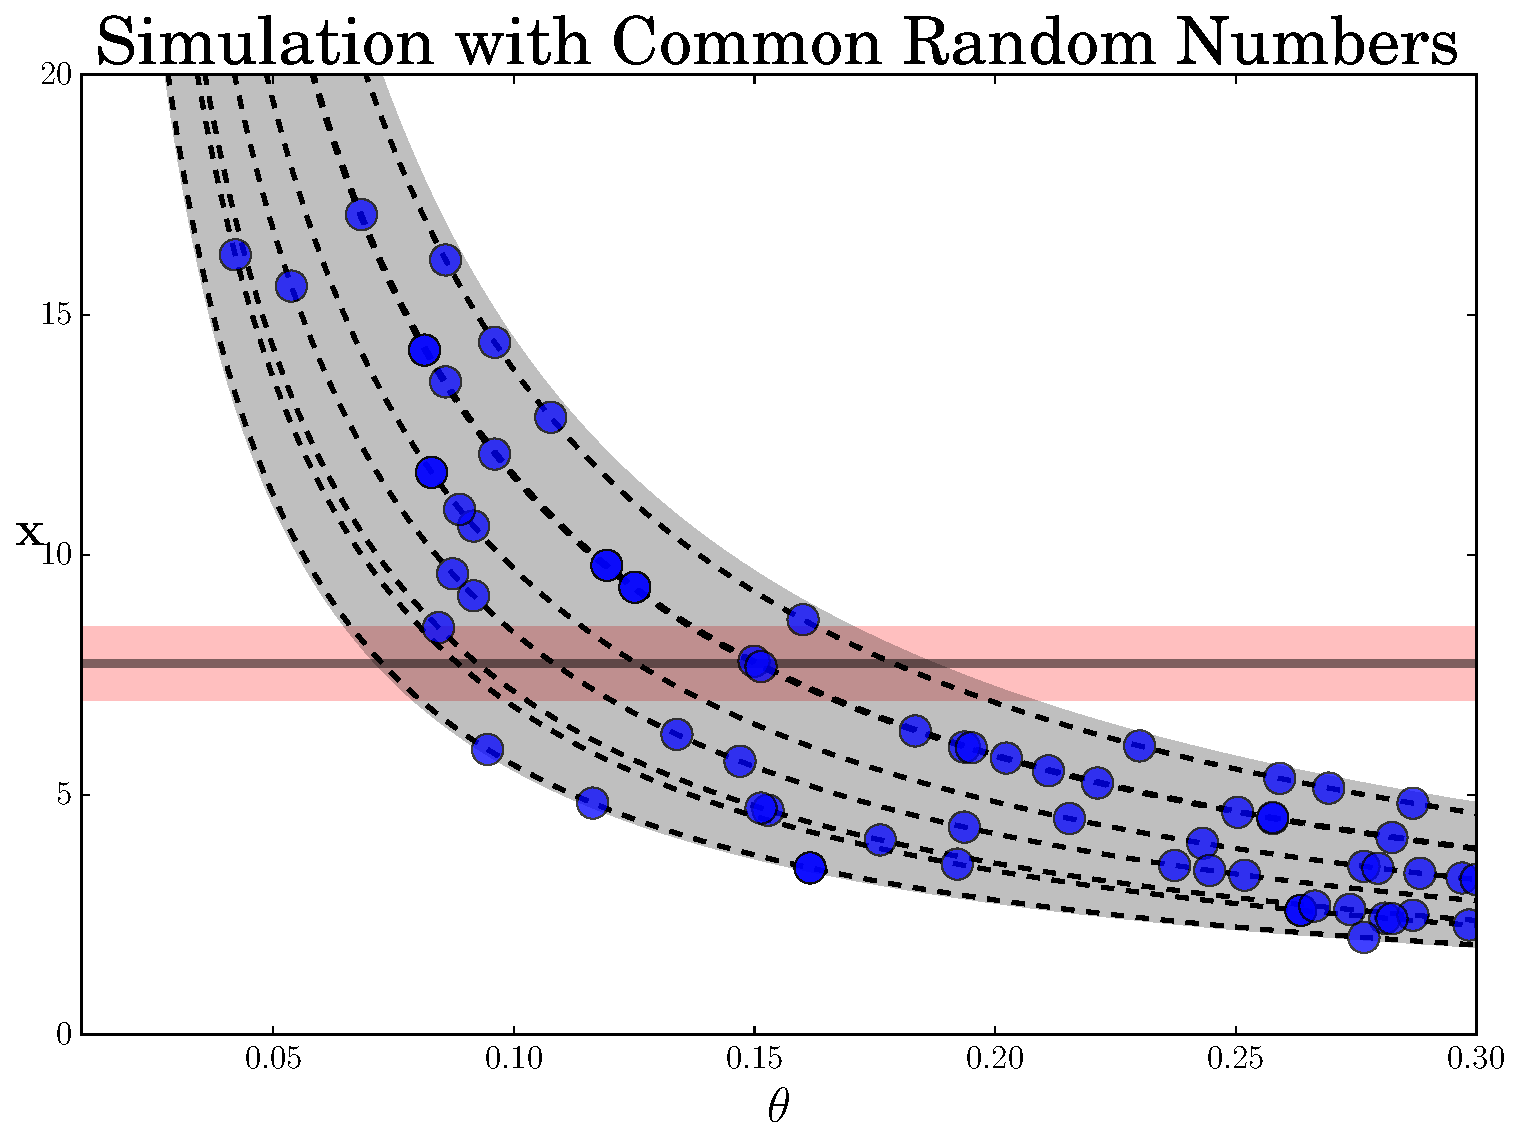
\includegraphics[width=0.95\columnwidth]{./images/exp_crn_figure.pdf}
\caption{\small{A view of a simulator in terms of common random numbers.  The horizontal line represents $\y$ and red shading $\pm 2\eps$.  The shaded curved region represents $2\sigma$ of $\pi(\x|\thetav)$.  The dashed lines are $f(\thetav, \omega_s)$ for several values of $\omega$.  The blue circles are potential random samples from $\pi(\x|\thetav)$.  For a fixed value $\omega_s$, the simulator produces deterministic outputs that change smoothly, even though the simulator itself is quite noisy.}}
\label{fig:exp-crns}
\end{center}
\vskip -0.2in
\end{figure} 

\begin{figure}[t]
\vskip 0.2in
\begin{center}
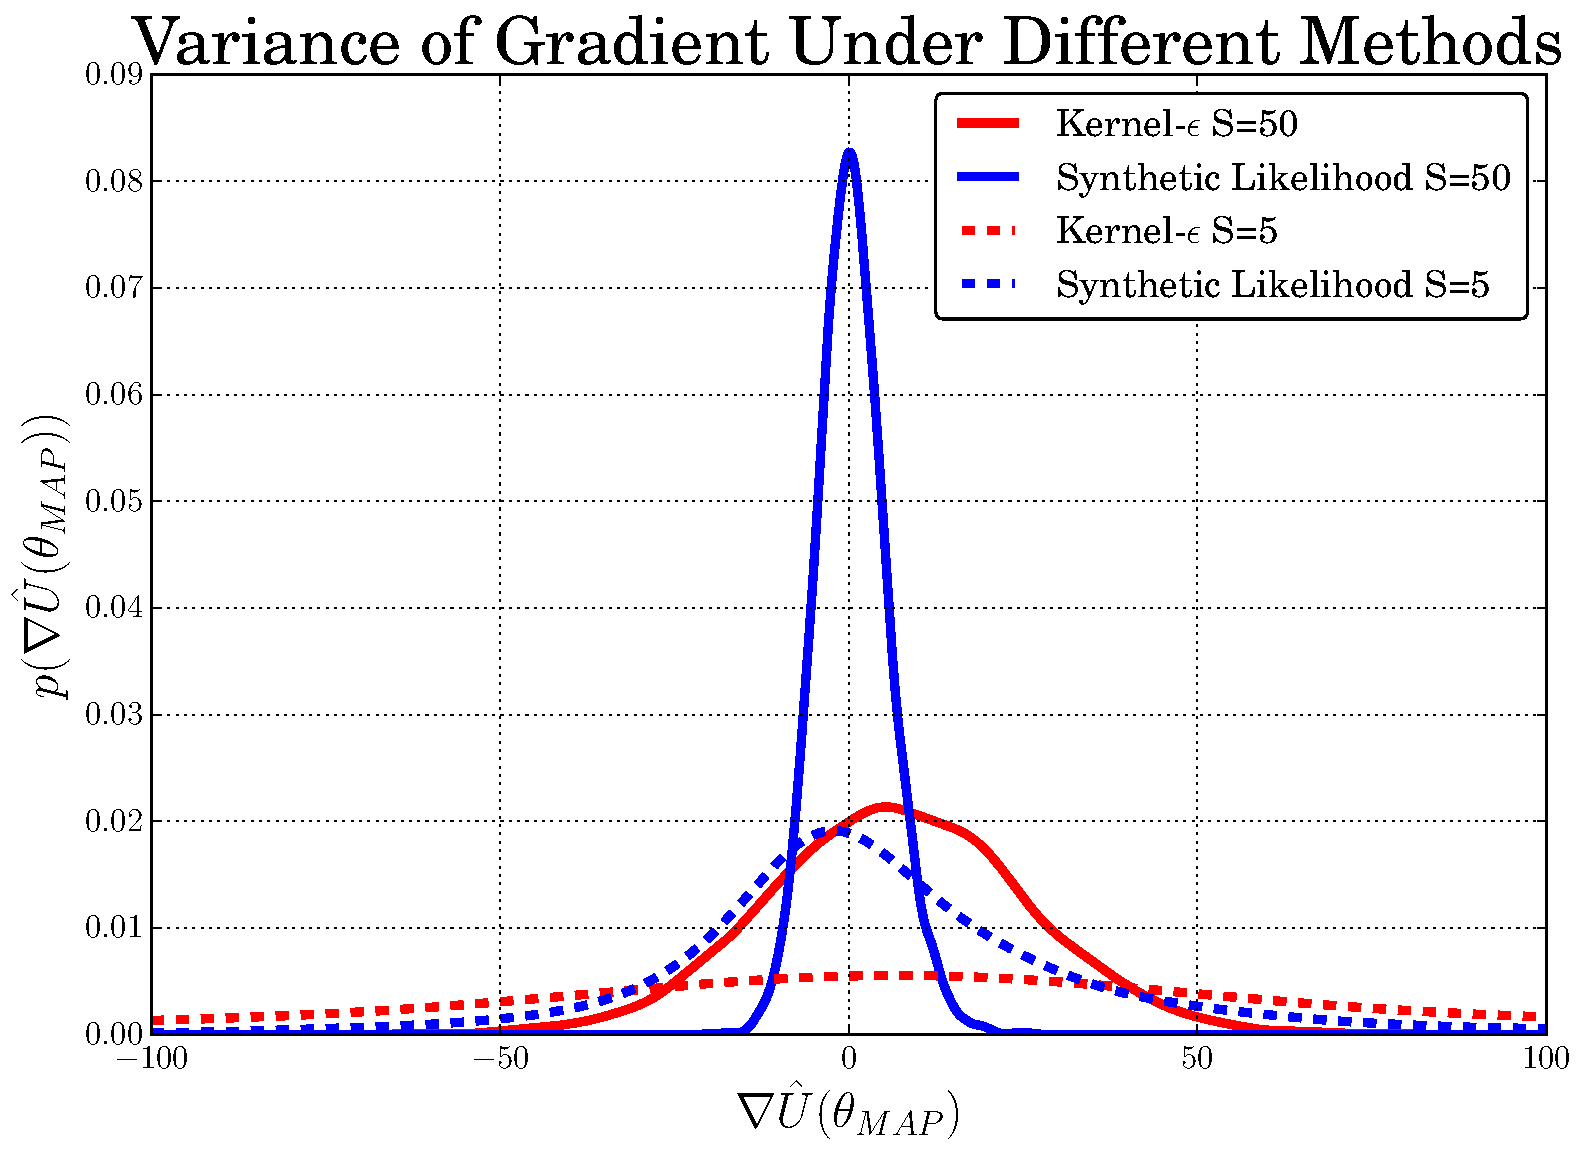
\includegraphics[width=0.95\columnwidth]{./images/exp_varg_figure.pdf}
\caption{\small{Variance of gradient estimation using kernel-$\eps$ and SL for different values of $S\in\{5,50\}$ and fixed $\eps = 0.37$ (the same used in the other results).  
%
When $S=5$, the empirical estimates of  $\nabla \hat{U}(\thetav_{\text{MAP}})$ are $-12 \pm 147$ (kernel-$\eps$) and $-9.3 \pm 43$ (SL).  When $S=50$ they are $-0.80 \pm 19$ (kernel-$\eps$) and $-7.3 \pm 4.9$ (SL).  Note the large discrepancy in variance.  Note the limit of $S \rightarrow \infty$,   $\nabla \hat{U}(\thetav_{\text{MAP}}) = -7.8$.  The bias if SL gradients is due to its Gaussian approximation (smoothed by $\eps$) of $\pi(\x|\thetav)$, which is a heavy-tailed Gamma distribution (the sum of $N$ exponentials).}}
\label{fig:exp-varg}
\end{center}
\vskip -0.2in
\end{figure}

\subsection{Common and Sticky Random Numbers}
The usefulness of using common random numbers (CRNS) for SPSA has been previously demonstrated \cite{kleinman1999simulation}.  In that work, the same random numbers are used to simulate both sides of the optimization function.  This makes sense intuitively, as we would generally assume that the expected simulation function changes smoothly with $d \thetav$;  by using CRNs, the smoothness can be captured by the gradient more easily (see Figure~\ref{fig:exp-crns}).  This is analogous to using the same mini-batch for both sides of the gradient computation, if we were to apply SPSA to Bayesian learning.  

In addition to using CRNs in simulations for each gradient computation, we have found that using persistent or {\em sticky} random numbers helps the HABC explore the parameter landscape more easily.  Intuitively, for a gradient-based sampling algorithm, it means a particle can slide along smooth Hamiltonian landscape because    the additive noise is suppressed.  This is very similar to using dependent random streams to drive MCMC \cite{Murray2012,Neal2012}, the main difference we believe is that we are using the Hamiltonian dynamics to drive proposals for $\thetav$ and using $\omegav$ suppress simulation noise.

  % , is within the gradient approximation so that the noise from the simulator has less of an influence that $\dtheta$.  In addition to this use, we have found that using the same random seeds over multiple time-steps improves the performance of HABC (TBD).  This is very similar to using dependent random streams to drive MCMC \cite{Murray2012,Neal2012}, the main difference we believe is that we are using the Hamiltonian dynamics to drive proposal in $\thetav$ and using $\omegav$ to give persistent simulations, reducing the variance from the unknown simulator noise function.
  
Using random seeds (versus, say, a set of random numbers) allows us to treat the simulator as a black-box, setting the random seed of its RNG without knowing the internal mechanisms it uses to generate random numbers.  We propose including persistent random seeds $\omegav$ in the state of our Markov chain.    As part of a Metropolis-Hastings transition operator, our idea is to randomly propose {\em flipping} each seed $\omega_s$ at time $t$ with some probability $\gamma$.  This implies that our simulation $\x^(s)$ changes automatically (as it is deterministic).  We argue that this is a valid transition operator using the similar arguments that can be made for pseudo-marginal ABC-MCMC which using equation~\ref{eq:pm-proposal} proposes $\thetavp$ and $\{ \x^{'(s)}\}$ jointly.  
This is equivalent to flipping all $\omegav$ {\em and} proposing $\thetavp$.  In ABC-MCMC, one could instead propose $q(\x^{'(s)} | \thetav)$ (fixing $\thetav$) and still sample correctly (this is like rejection sampling $\x | \y, \thetav$ based on $\epsvec$).  What we propose is slightly different.  Again keeping $\thetav$ fixed, we propose new random seeds with some probability $\gamma$ from some uniform prior distribution over seeds.  The Metropolis-Hastings ratio reduces to the ratio of likelihoods for observations $\y$ given the new deterministic simulation values (just like it would for ABC-MCMC).  By keeping the random seeds fixed, we can sample $\thetav$ using HABC and use $\omegav$ as CRNs within the gradient computation step.

% Our updates for $\omegav$ are simple.  At each time step $t$, each seed is refreshed to a new random value with probability $\gamma$, i.e. $\omega_s \leftarrow \omega_s$ with probability $\gamma$, and $\omega_s \leftarrow \mathcal{U}(1,W)$, where $W=10^8$ in our algorithms.  By observing the simulation at different $\thetav$ but using same seeds, we can eliminate much of the simulator noise from the Markov chain.  By treating $\omegav$ as part of the state of the Markov chain, we can smoothly move along noiseless outputs for several iterations and then propose new seeds.  Though proposing new seeds produces a valid Metropolis-Hastings algorithm (keeping $\thetav$ fixed and changing $\omegav$), we found that using {\em sticky} random seeds works well.  These seeds can be precomputed before the chain is run and can be seen as apart from the state of the Markov chain.  [CONFUSING]

%[We may want anti-thetic instead of CRNs, ie overrelax versus underrelax, etc.]
\begin{figure}[t]
\vskip 0.2in
\begin{center}
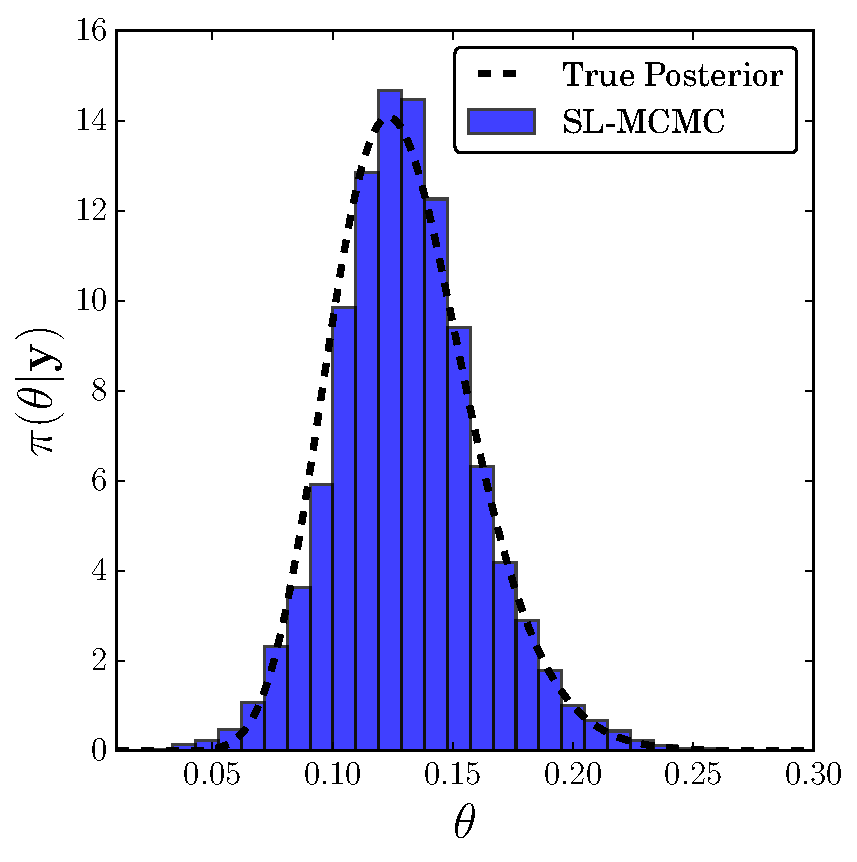
\includegraphics[width=0.32\columnwidth]{./images/exp-SL-MCMC-posterior-hist-omega-rate-100p0-chain0.pdf}
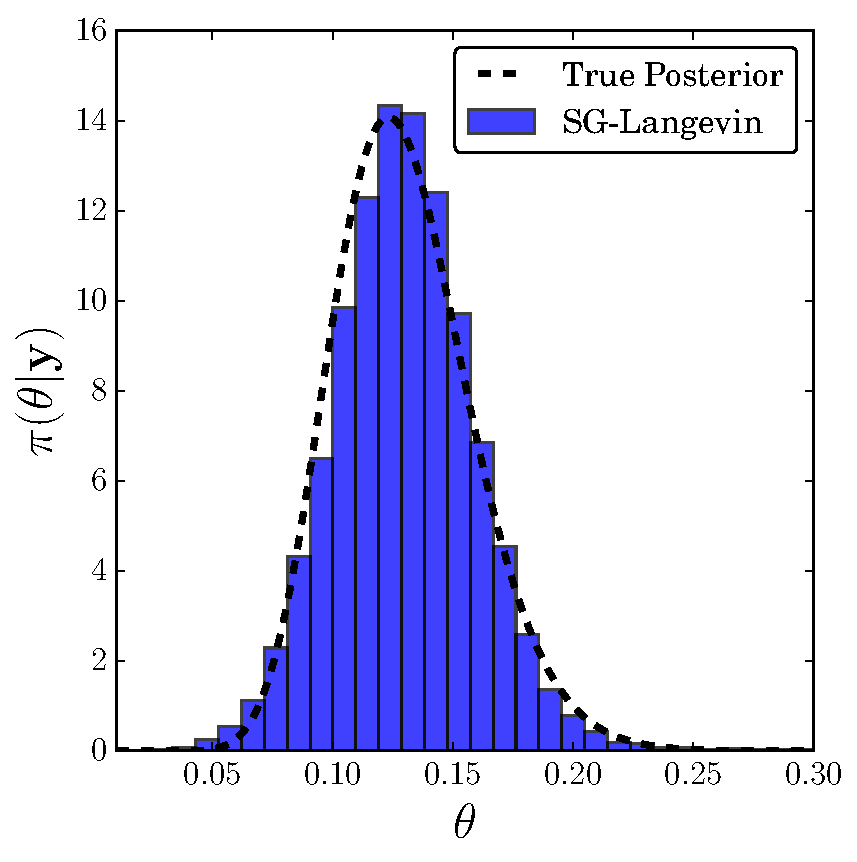
\includegraphics[width=0.32\columnwidth]{./images/exp-SG-Langevin-posterior-hist-omega-rate-100p0-chain0.pdf}
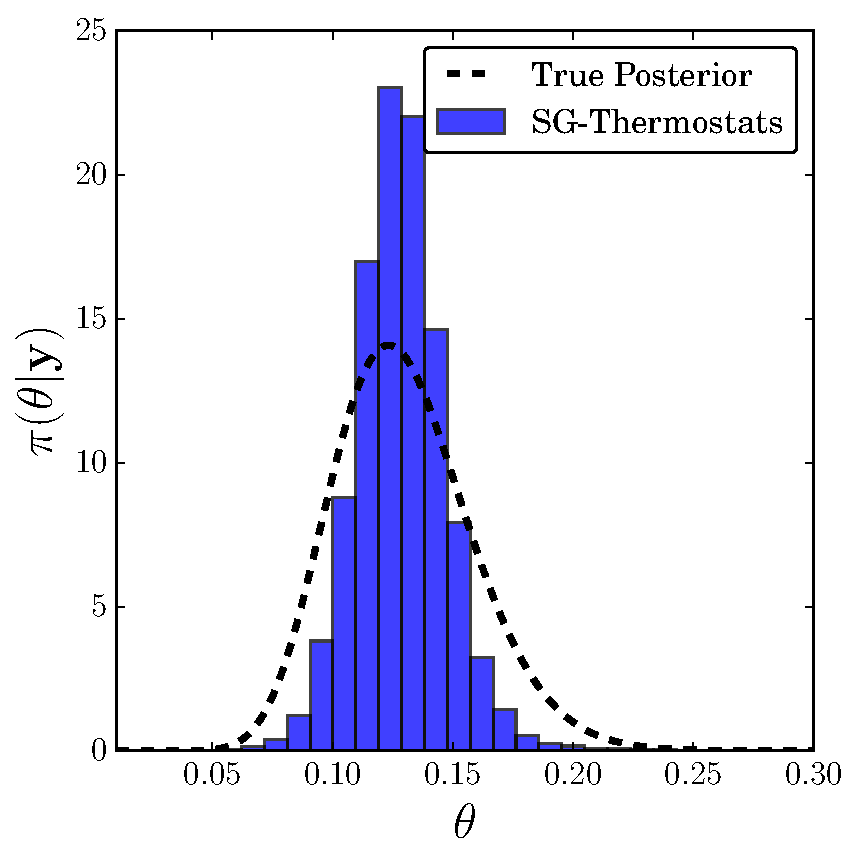
\includegraphics[width=0.32\columnwidth]{./images/exponential/exp3-SG-Thermostats-posterior-hist-omega-rate-100p0-chain0.pdf}

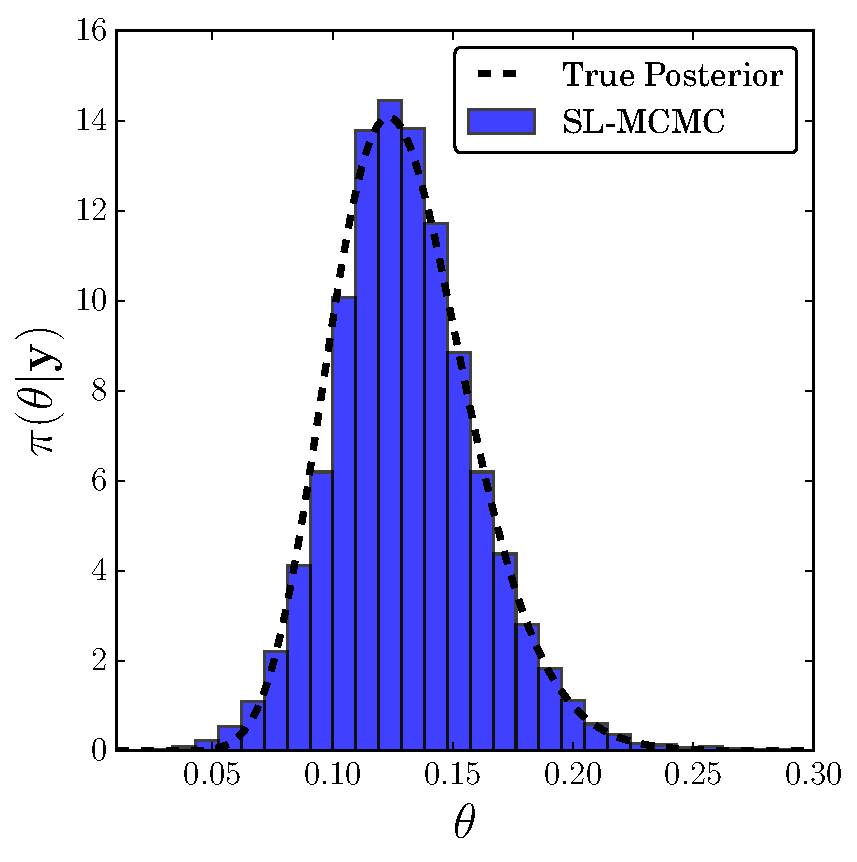
\includegraphics[width=0.32\columnwidth]{./images/exponential/exp2-SL-MCMC-posterior-hist-omega-rate-0p1-chain1.pdf}
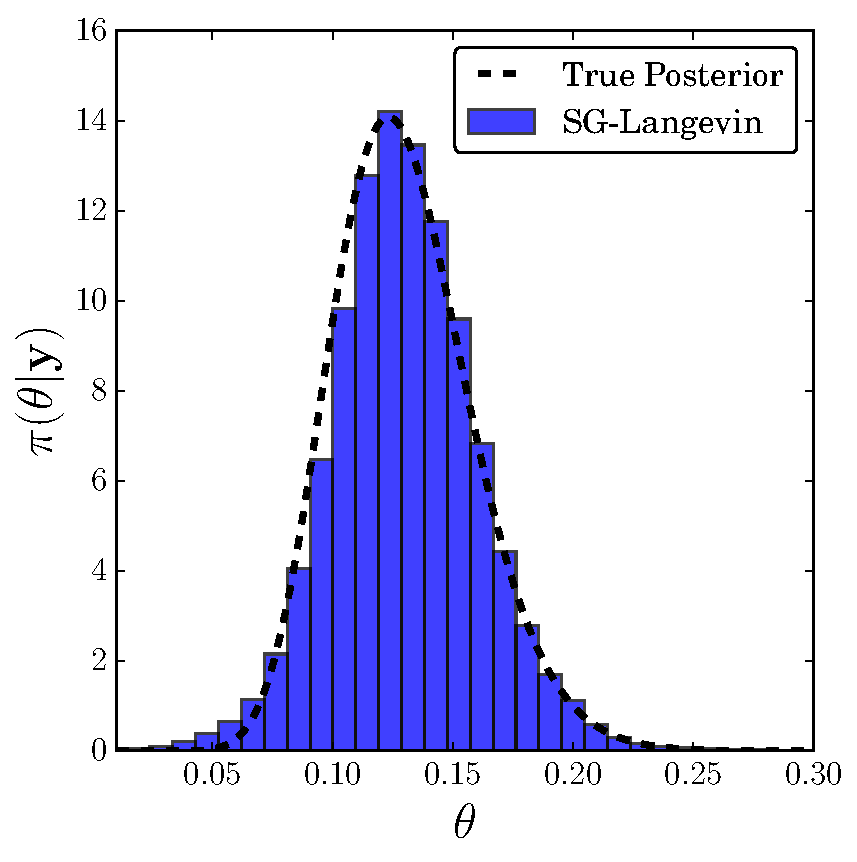
\includegraphics[width=0.32\columnwidth]{./images/exponential/exp2-SG-Langevin-posterior-hist-omega-rate-0p1-chain0.pdf}
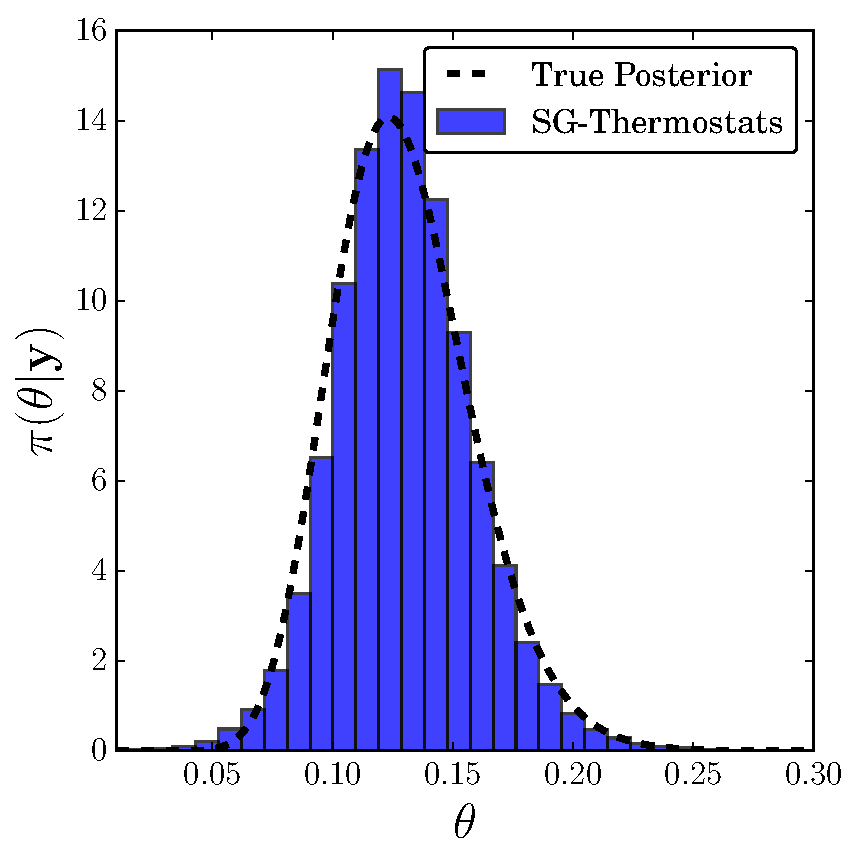
\includegraphics[width=0.32\columnwidth]{./images/exponential/exp2-SG-Thermostats-posterior-hist-omega-rate-0p1-chain1.pdf}

%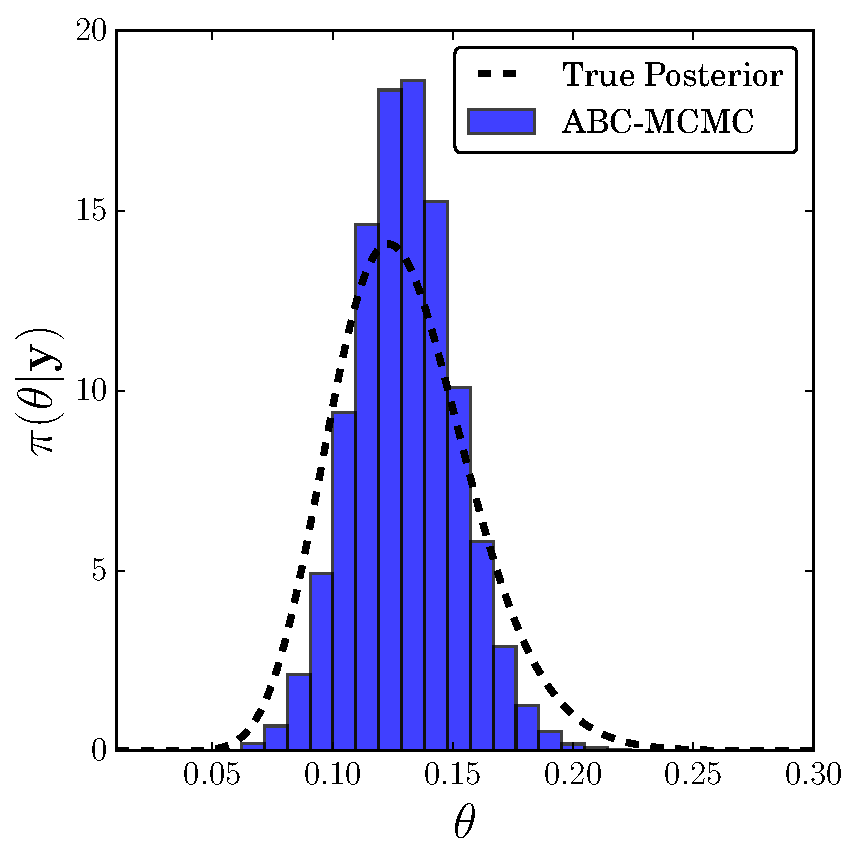
\includegraphics[width=0.45\columnwidth]{./images/exp-ABC-MCMC-posterior_hist.pdf}
%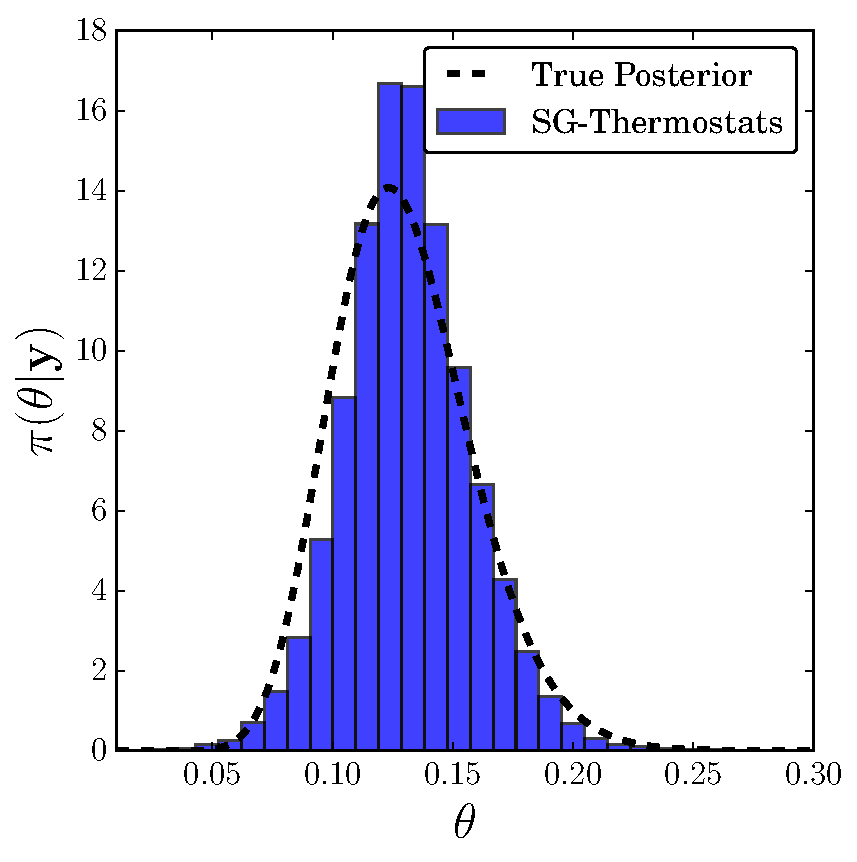
\includegraphics[width=0.45\columnwidth]{./images/exp-SG-Thermostats-posterior_hist.pdf}
%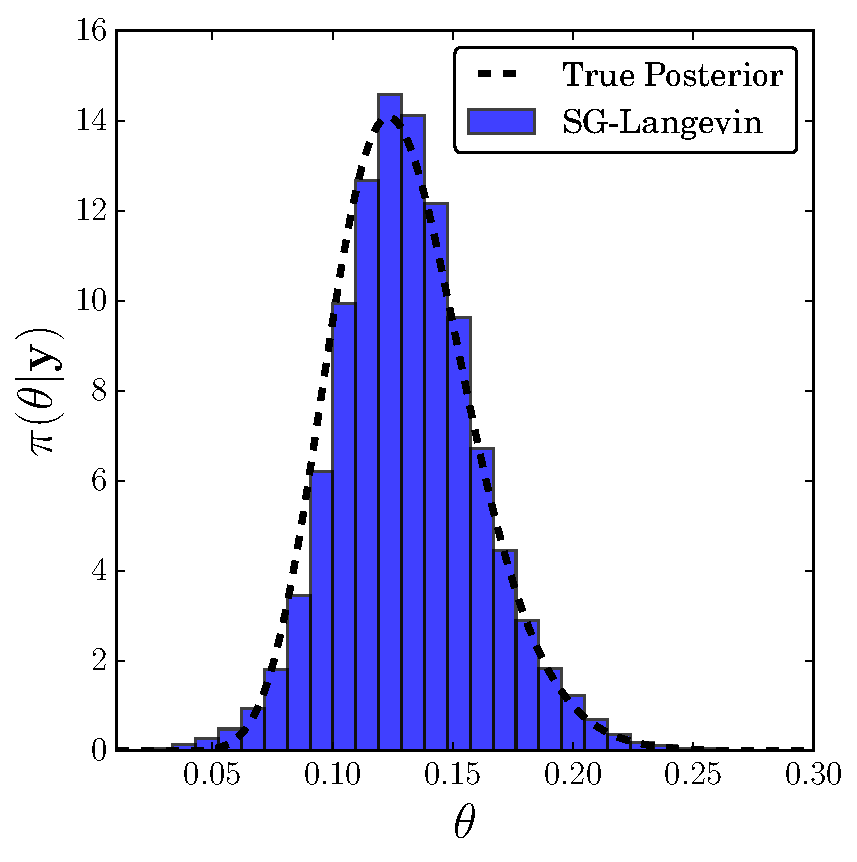
\includegraphics[width=0.45\columnwidth]{./images/exp-SG-Langevin-posterior_hist.pdf}
%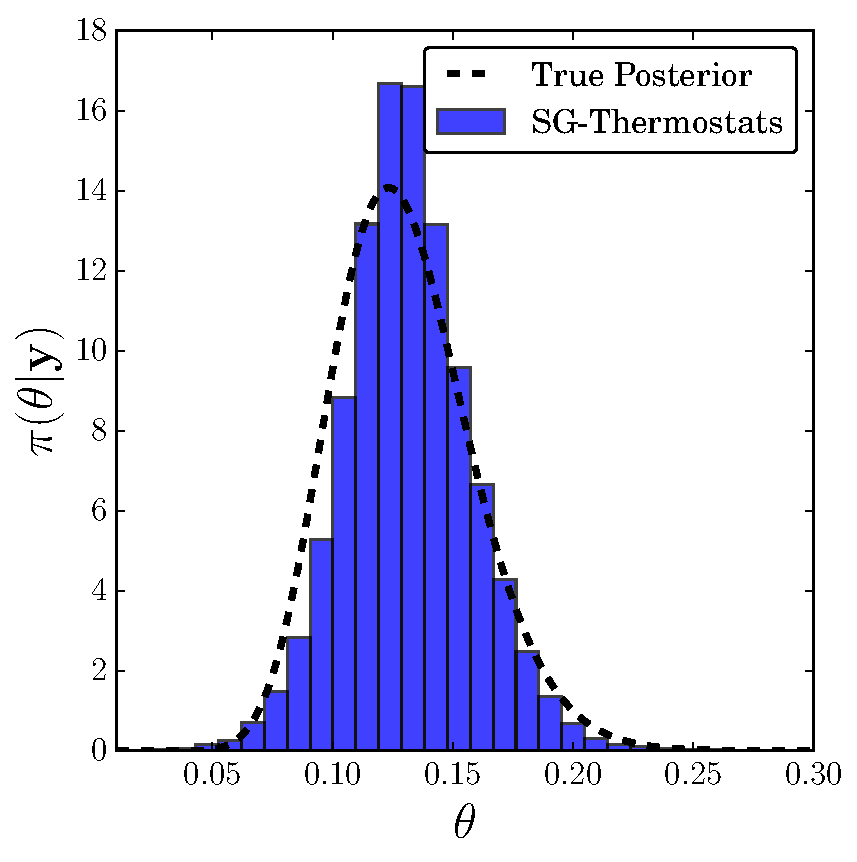
\includegraphics[width=0.45\columnwidth]{./images/exp-SG-Thermostats-posterior_hist.pdf}
\caption{\small{Posterior distributions for the demonstration problem.  {\bf Top row:} No persistent seeds.  {\bf Bottom row:} Persistent seeds with $\gamma=0.1$.  Histograms of the posterior estimates are overlaid with the true posterior (dashed line).  All algorithms (except for SG-Thermostats for non-persistent $\omegav$) give roughly the same posterior estimate.  By adding persistent $\omegav$ SG-Thermostats achieved similar posteriors to the other algorithms.}}
\label{fig:exp-posteriors}
\end{center}
\vskip -0.2in
\end{figure} 
%
% \begin{figure}[t]
% \vskip 0.2in
% \begin{center}
% 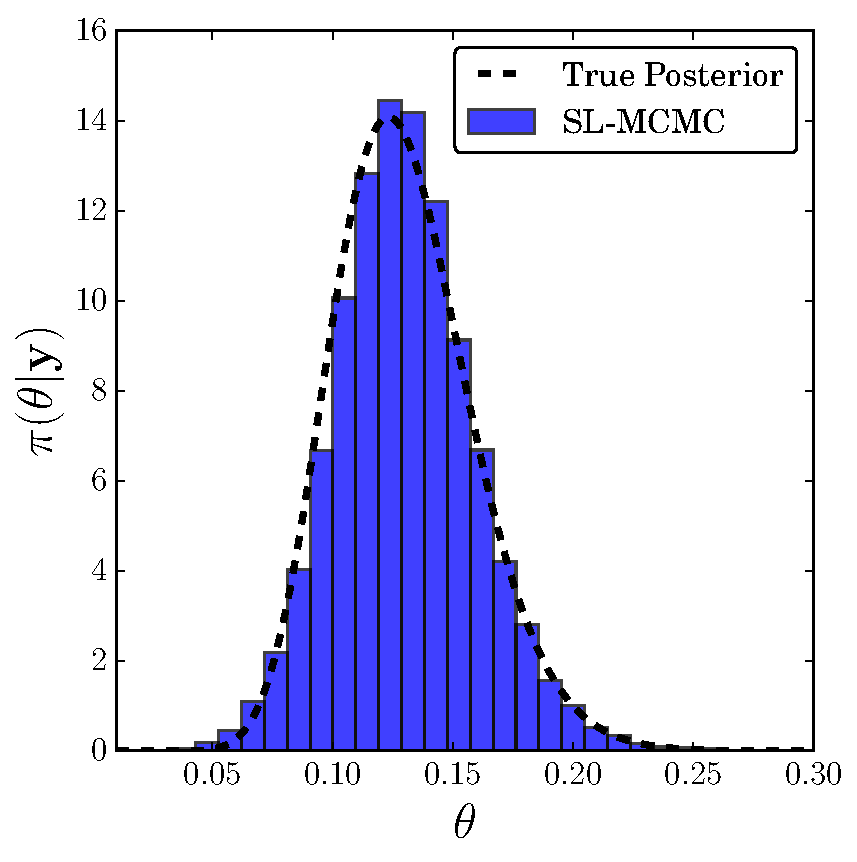
\includegraphics[width=0.45\columnwidth]{./images/exp-SL-MCMC-posterior-hist-omega-rate-0p01-chain0.pdf}
% 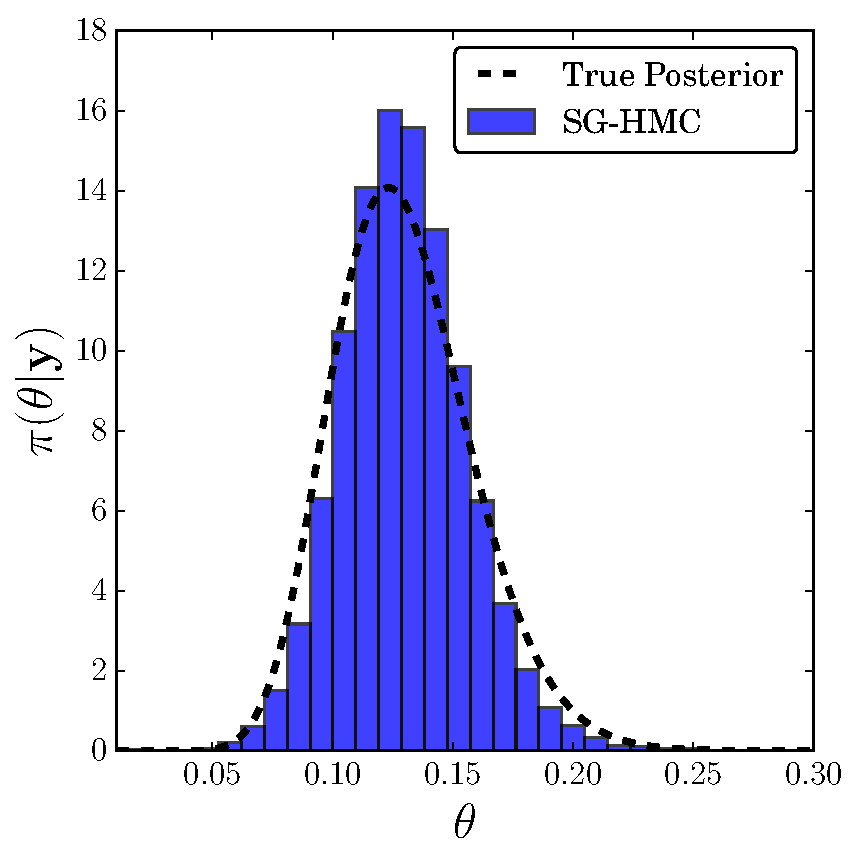
\includegraphics[width=0.45\columnwidth]{./images/exp-SG-HMC-posterior-hist-omega-rate-0p01-chain0.pdf}
% 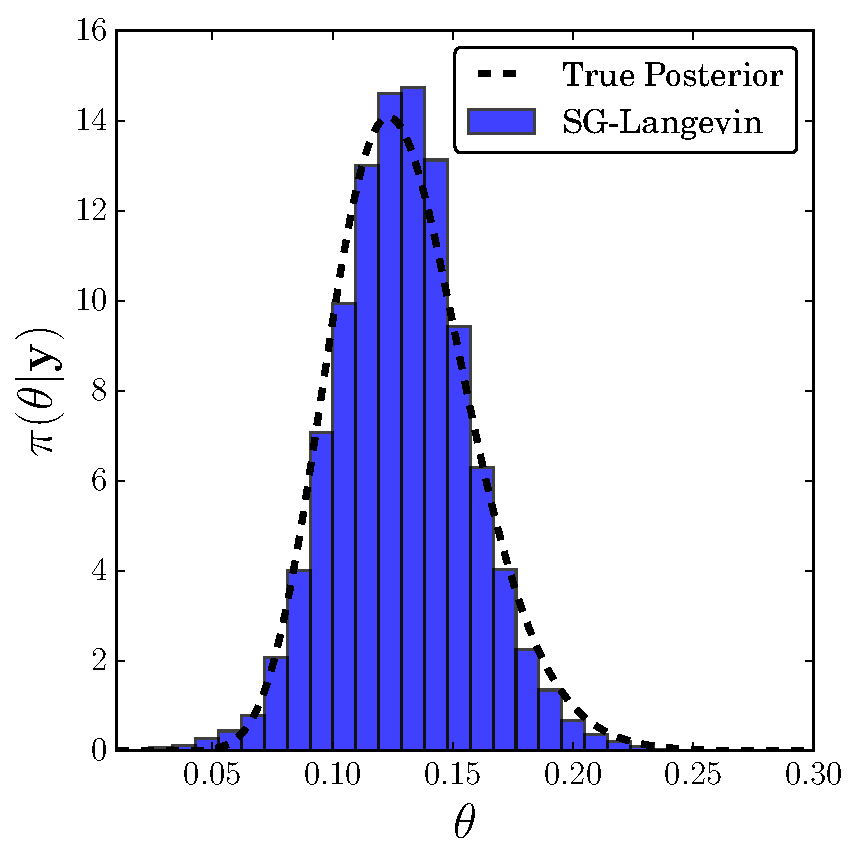
\includegraphics[width=0.45\columnwidth]{./images/exp-SG-Langevin-posterior-hist-omega-rate-0p01-chain0.pdf}
% 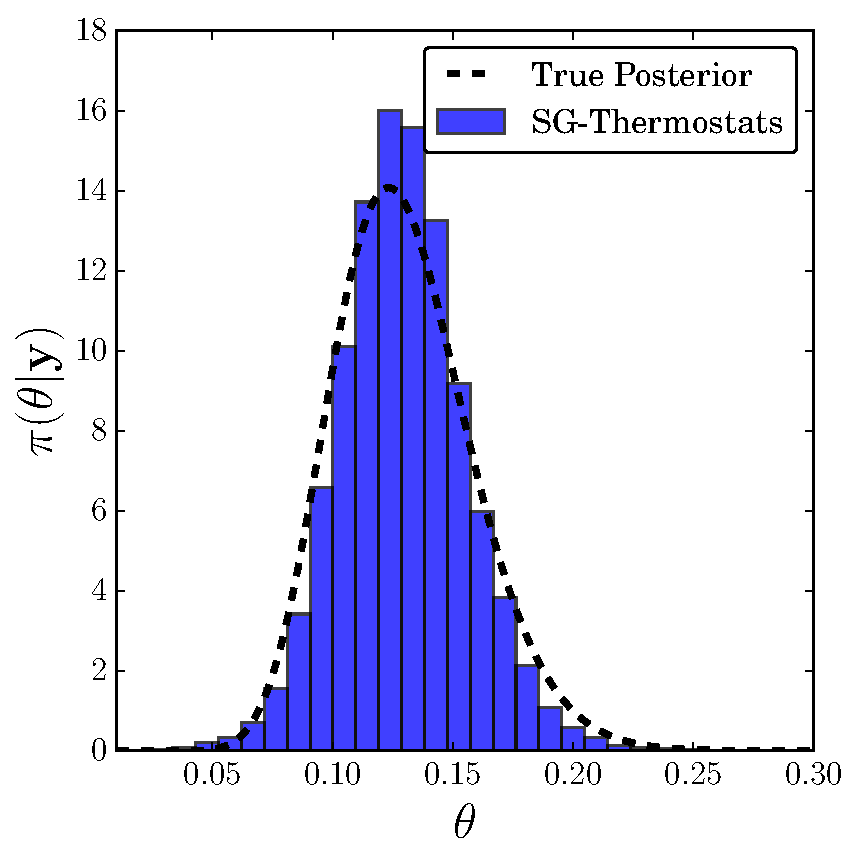
\includegraphics[width=0.45\columnwidth]{./images/exp-SG-Thermostats-posterior-hist-omega-rate-0p01-chain0.pdf}
% %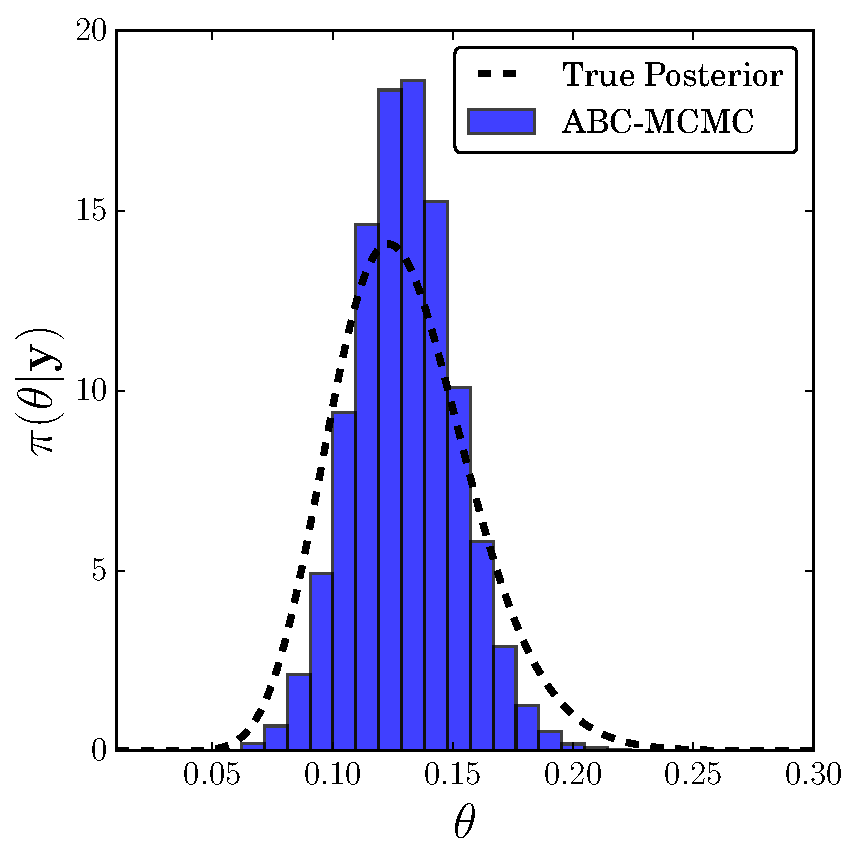
\includegraphics[width=0.45\columnwidth]{./images/exp-ABC-MCMC-posterior_hist.pdf}
% %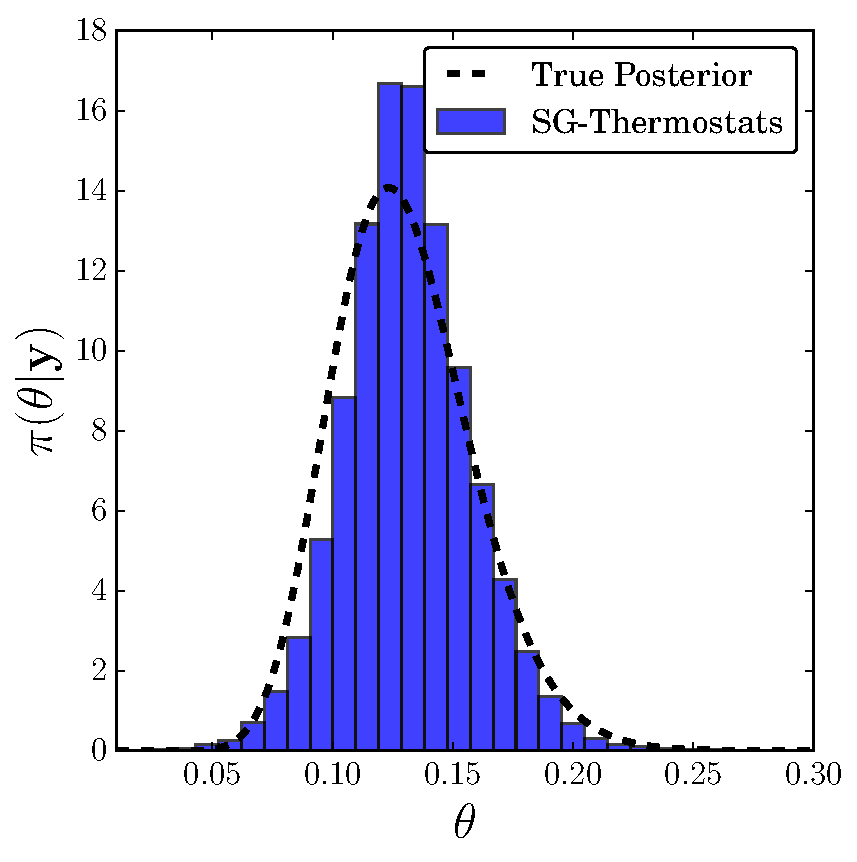
\includegraphics[width=0.45\columnwidth]{./images/exp-SG-Thermostats-posterior_hist.pdf}
% %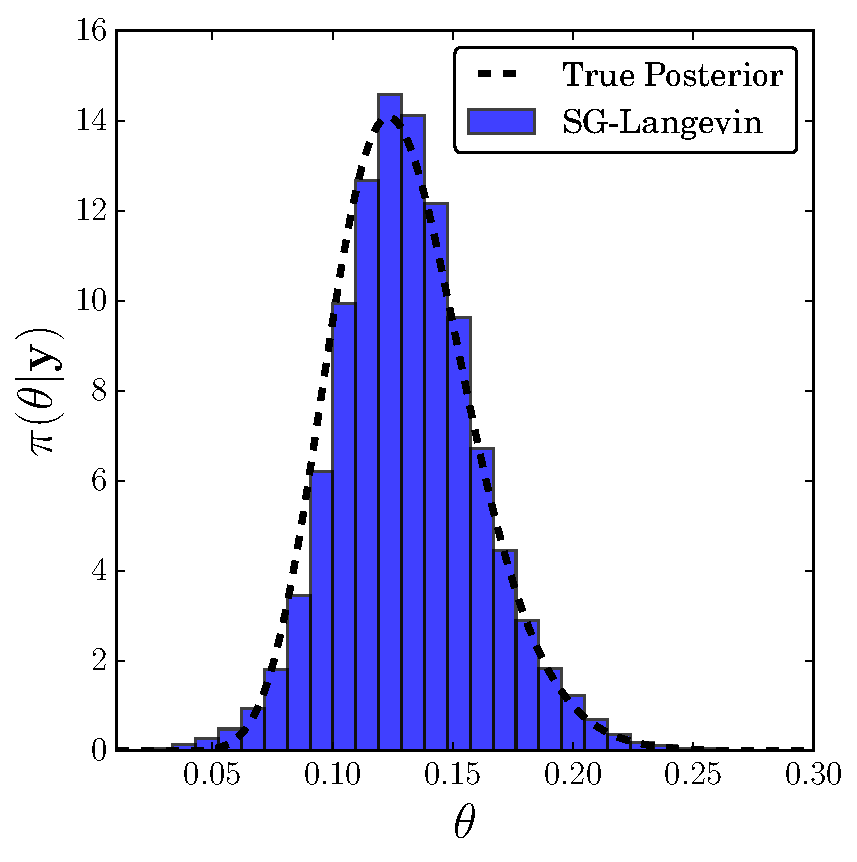
\includegraphics[width=0.45\columnwidth]{./images/exp-SG-Langevin-posterior_hist.pdf}
% %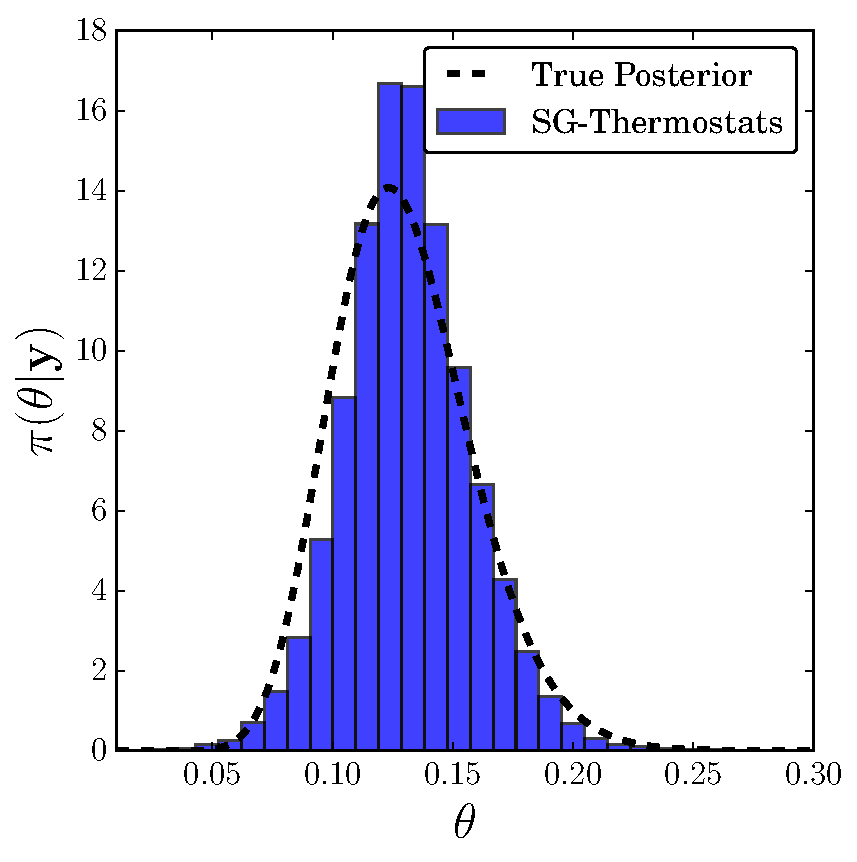
\includegraphics[width=0.45\columnwidth]{./images/exp-SG-Thermostats-posterior_hist.pdf}
% \caption{\small{Using sticky numbers at rate $1\%$}}
% \label{fig:exp-posteriors}
% \end{center}
% \vskip -0.2in
% \end{figure}



%%%%%%%%%%%%%%%%%%%%%%%%%%%%%%%%%%%%%%%%%%%%%%%%%
\section{Demonstration}\label{sec:demo}
%%%%%%%%%%%%%%%%%%%%%%%%%%%%%%%%%%%%%%%%%%%%%%%%%
We use a simple $D=1$ problem to demonstrate HABC.  Let $y= \frac{1}{N} \sum_{i} e_i$, where $e_i \sim \text{Exp}(1/\thetastar)$; $\thetastar = 0.15$, $N=20$, and $y=7.74$ in our concrete example.  Assuming $\pi(\theta ) = \text{Gamma}(\alpha, \beta)$, the true posterior is a gamma distribution with shape $\alpha+N$ and rate $\beta + N y$.  Our simulator therefore generates the average of $N$ exponential random variates with rate $\lambda = 1/\theta$.  Data $x \simsim \pi(x|\theta)$ are shown in Figure~\ref{fig:exp-crns}.  We have explicitly shown the smoothness of the simulator by generating data along trajectories of fixed seeds $\omega_s$; i.e. for several $\omega_s$ we vary $\theta$ (dashed lines are function $f(\theta, \omega_s)$) and randomly reveal data (blue circles).  The horizontal line with shading indicates $y \pm 2 \eps$, where $\eps = 0.37$ is used throughout the demonstration.



% \begin{figure*}[t]
% %\vskip 0.2in
% \setlength{\linewidth}{\textwidth}
% \setlength{\hsize}{\textwidth}
% \begin{center}
% 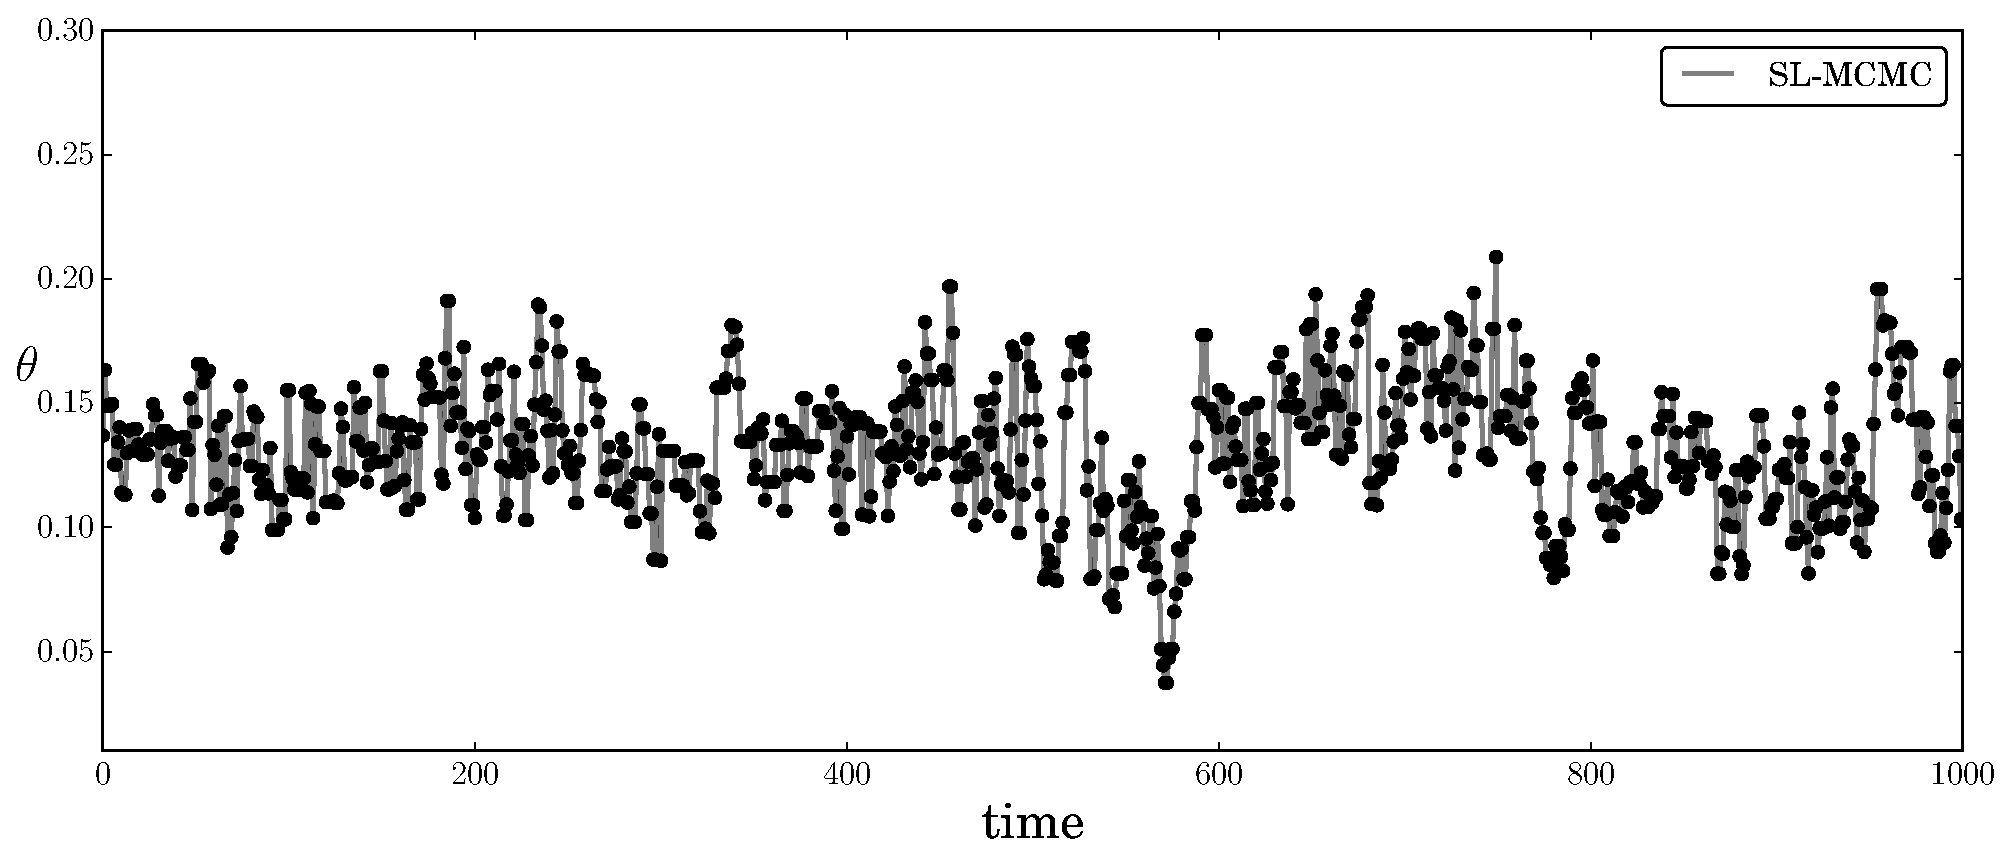
\includegraphics[width=0.95\columnwidth]{./images/exp-SL-MCMC-theta-timeseries-omega-rate-0p01-chain0.pdf}
% %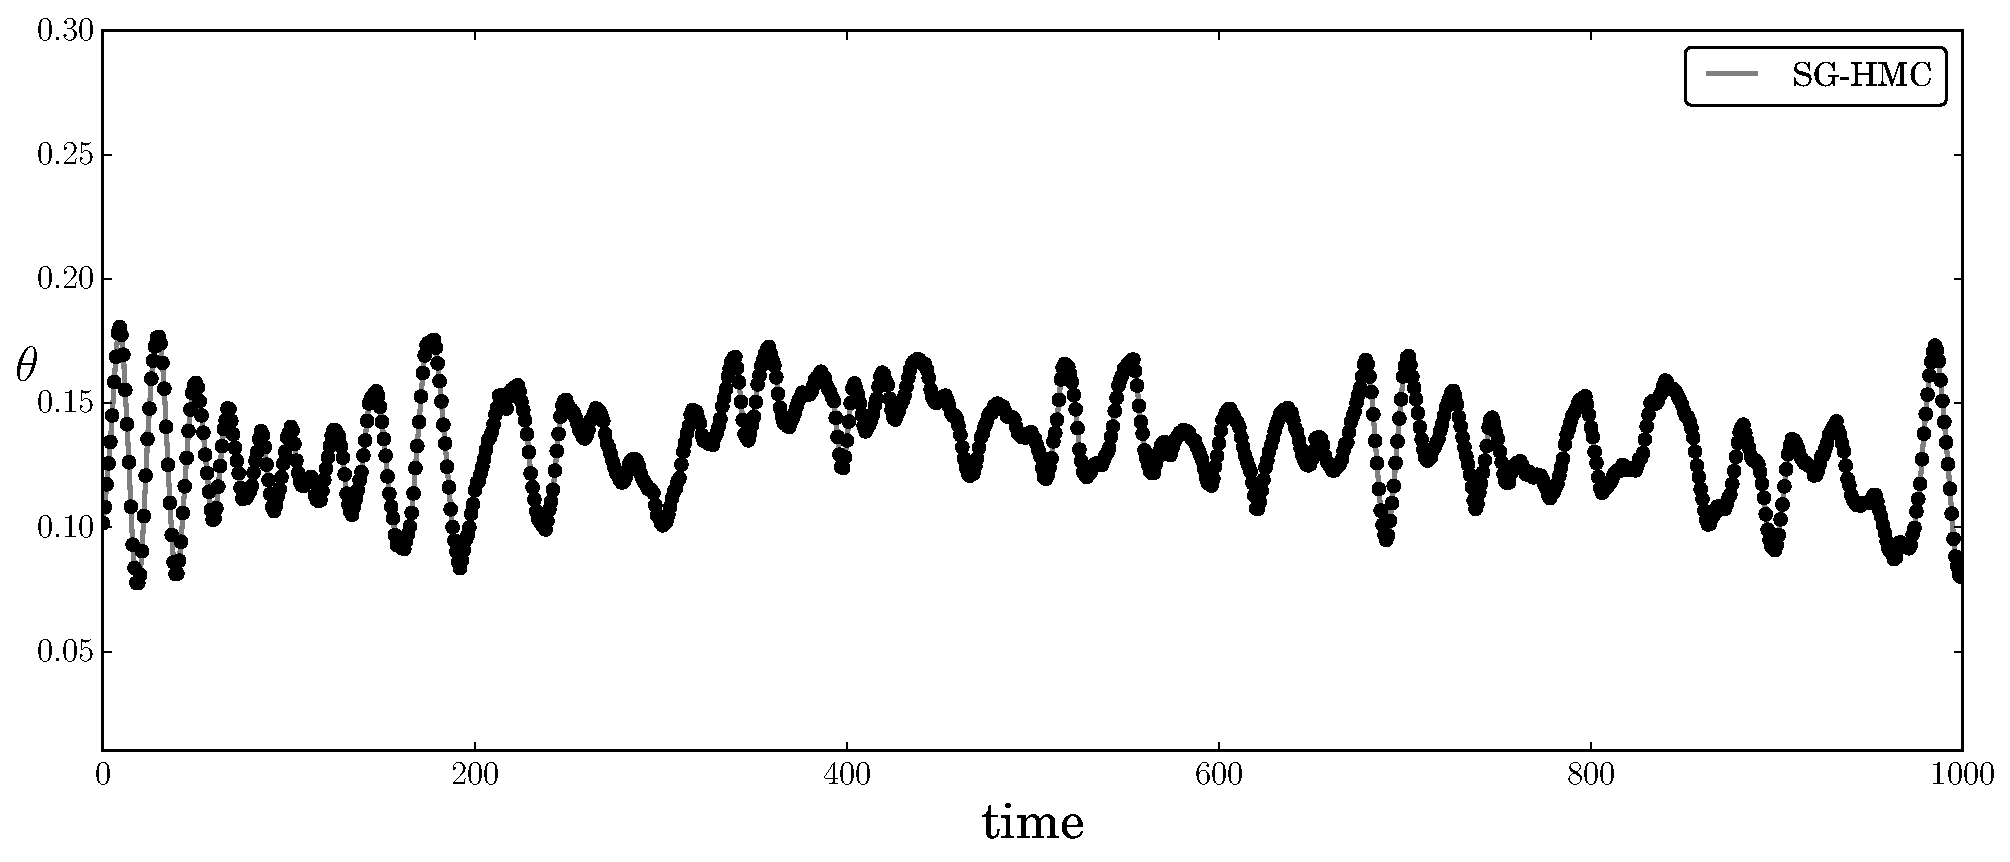
\includegraphics[width=0.95\columnwidth]{./images/exp-SG-HMC-theta-timeseries-omega-rate-0p01-chain0.pdf}
% 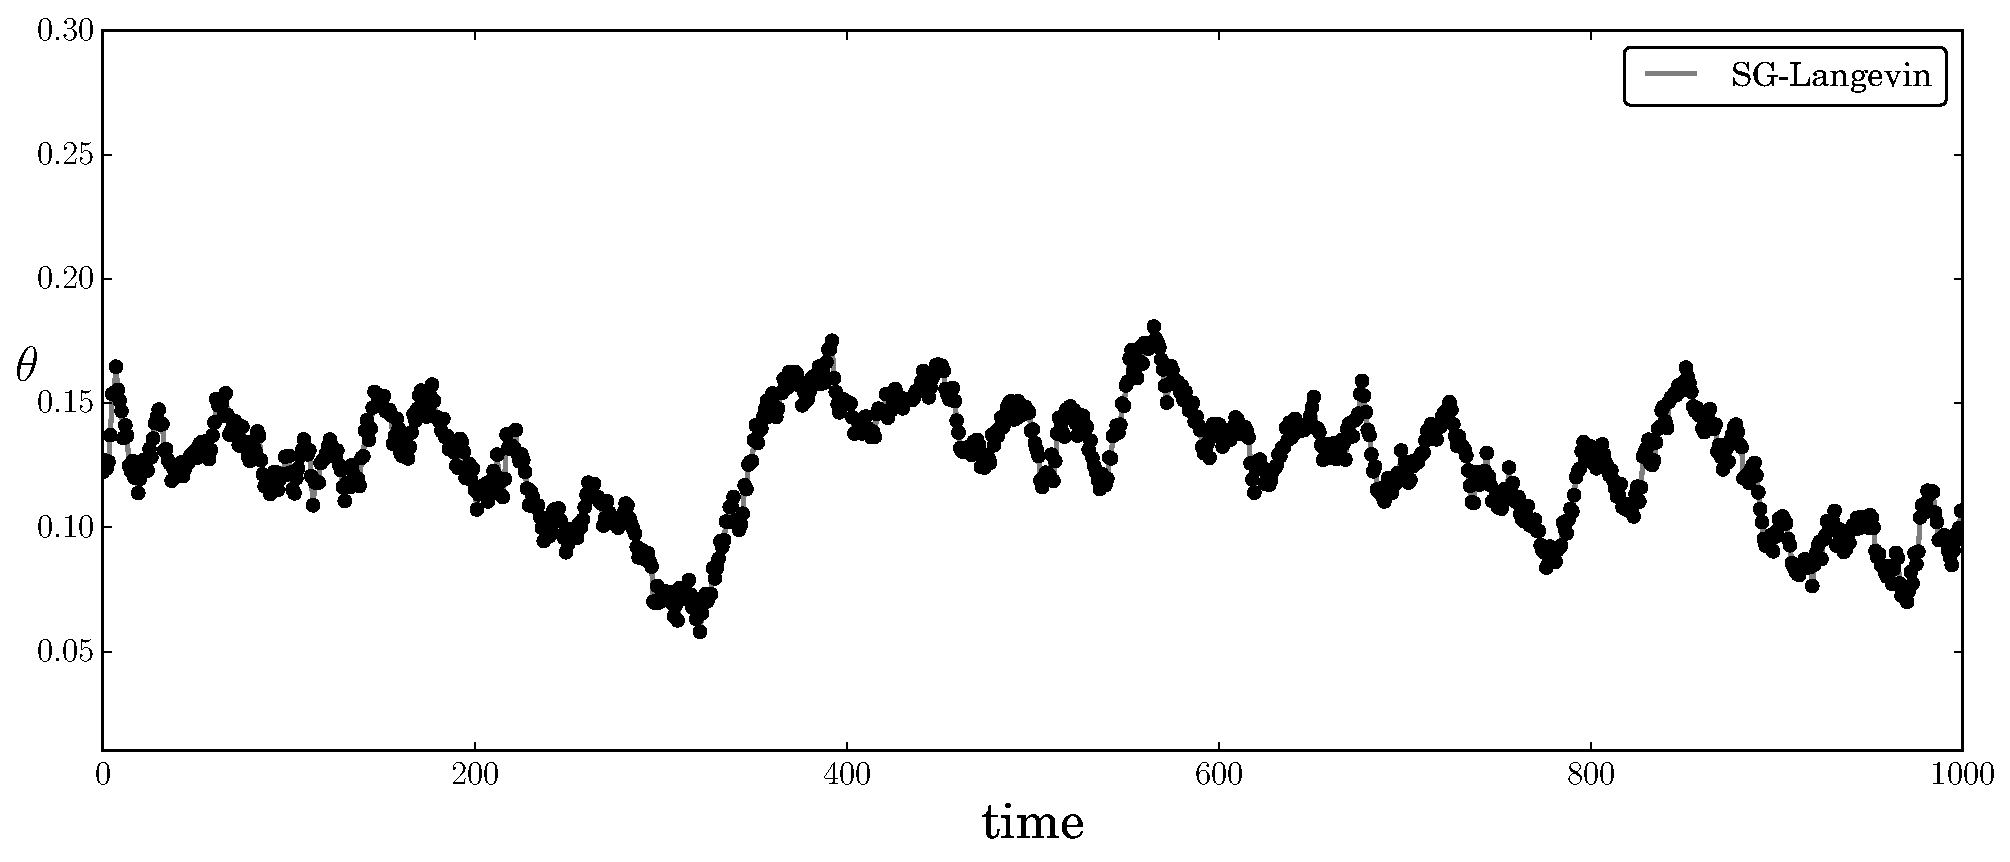
\includegraphics[width=0.95\columnwidth]{./images/exp-SG-Langevin-theta-timeseries-omega-rate-0p01-chain0.pdf}
% 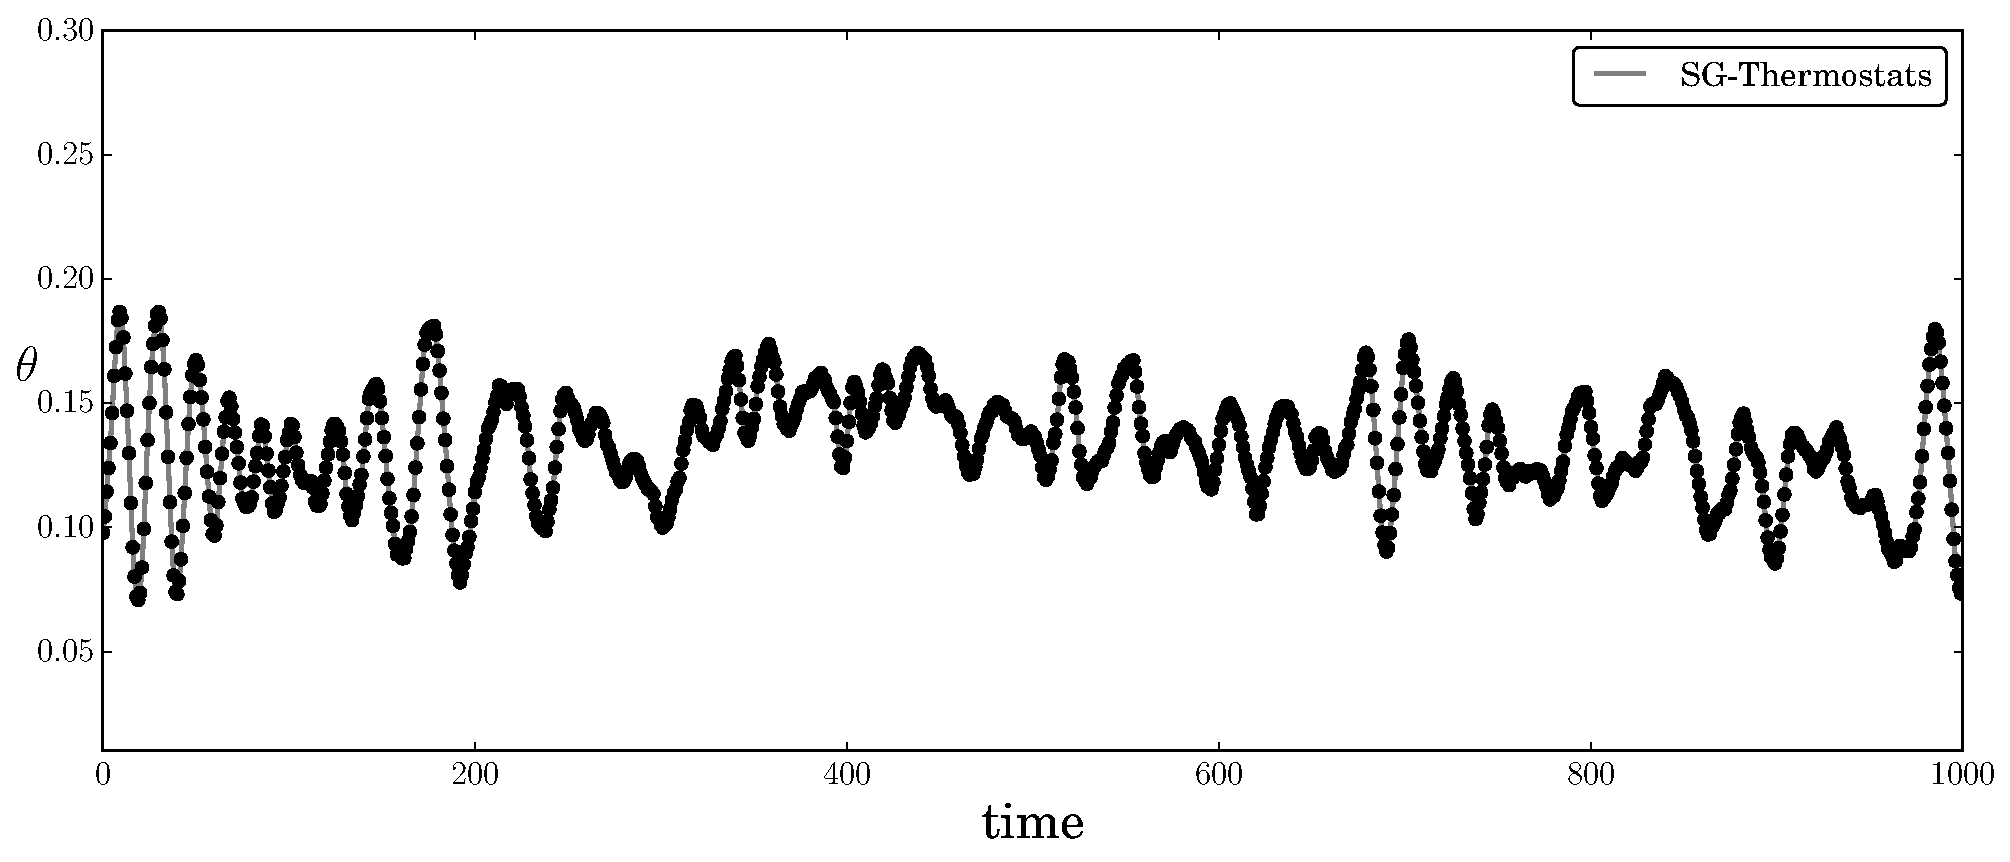
\includegraphics[width=0.95\columnwidth]{./images/exp-SG-Thermostats-theta-timeseries-omega-rate-0p01-chain0.pdf}
% \caption{\small{Using sticky numbers at rate $1\%$}}
% \label{fig:exp-theta-traces}
% \end{center}
% \vskip -0.2in
% \end{figure*}

 



\subsection{Bias and Variance of $\nabla \hat{U}(\thetav)$}
To test our assumption that the SL likelihood is better suited for HABC, we ran FDSA at the true $\theta_{\text{MAP}}$.  Using $S=5$ and $S=50$ and fixing $\eps = 0.37$, we gather $10K$ gradients samples using kernel-$\epsvec$ and SL likelihoods.  These gradient estimate densities are shown in Figure~\ref{fig:exp-varg}.  An unbiased estimate of the gradient should be centered at $0$.  There are two important results.  First, the SL estimates have a small bias, even at $S=50$.  This is because it is estimating the true Gamma distribution of $\pi(\x|\thetav)$ with a Gaussian.  We can analytically estimate this bias as $S \rightarrow \infty$; for this example it is $-7.8$ which is what SL estimates are centered around ($-9.3$ for $S=5$ and $7.3$ for $S=50$).  The kernel-$\epsvec$ likelihood has very low bias at $S=50$ (but large at $S=5$, $-12$).  However, the second important result is the variances.  SL variances decrease quickly with $S$: $\sigma^2 = 43^2 \rightarrow 4.9^2$, whereas kernel-$\epsvec$ starts very high and remains much higher: $\sigma^2 = 147^2 \rightarrow 19^2$.  It is for this reason that we have chosen to use SL likelihoods for our gradient estimates, despite their small bias. As mentioned in Section~\ref{sec:habc-grads} it is possible that other likelihood models, such as KDE, might provide low bias and low variance gradient estimates.  We leave this for future work.
%
%
% [REWRITE] At $\theta_{\text{MAP}}$ we estimated the gradient $\nabla \hat{U}(\theta)$ using finite differences for both the kernel-$\epsilon$ and synthetic-likelihood representation of $\pi_{\eps}(y | x )$.  For $S=5$ and $S=50$, $10K$ repetitions of computing the gradients was performed; there histograms are shown in Figure~\ref{fig:exp-varg}.  At $S=5$ both methods reveal a small bias (values X and Y for kernel-$\eps$ and SL, respectively).  At $S=50$, the bias for kernel-$\eps$ is much smaller, but its variance remains high; for SL, the bias remains unchanged but the variance has decreased significantly (values X pm S and Y pm T). The bias in the SL representation comes from the Gaussian approximation $\pi(y|\theta)$ which we can compute analytically using the CLT as $\text{N}( 1/\theta, 1/N \theta^2 + \eps^2)$.
% (We believe this bias is due to the normal approximation assuming a symmetric mode as the bias goes to zero at the mean of the true posterior).  Note that this bias is directional signal only appears nears the mode.  For the $S=5$ setting in our experiment both approaches contain similar bias. [REWRITE END]


\begin{figure*}[t]
%\vskip 0.2in
\setlength{\linewidth}{\textwidth}
\setlength{\hsize}{\textwidth}
\begin{center}
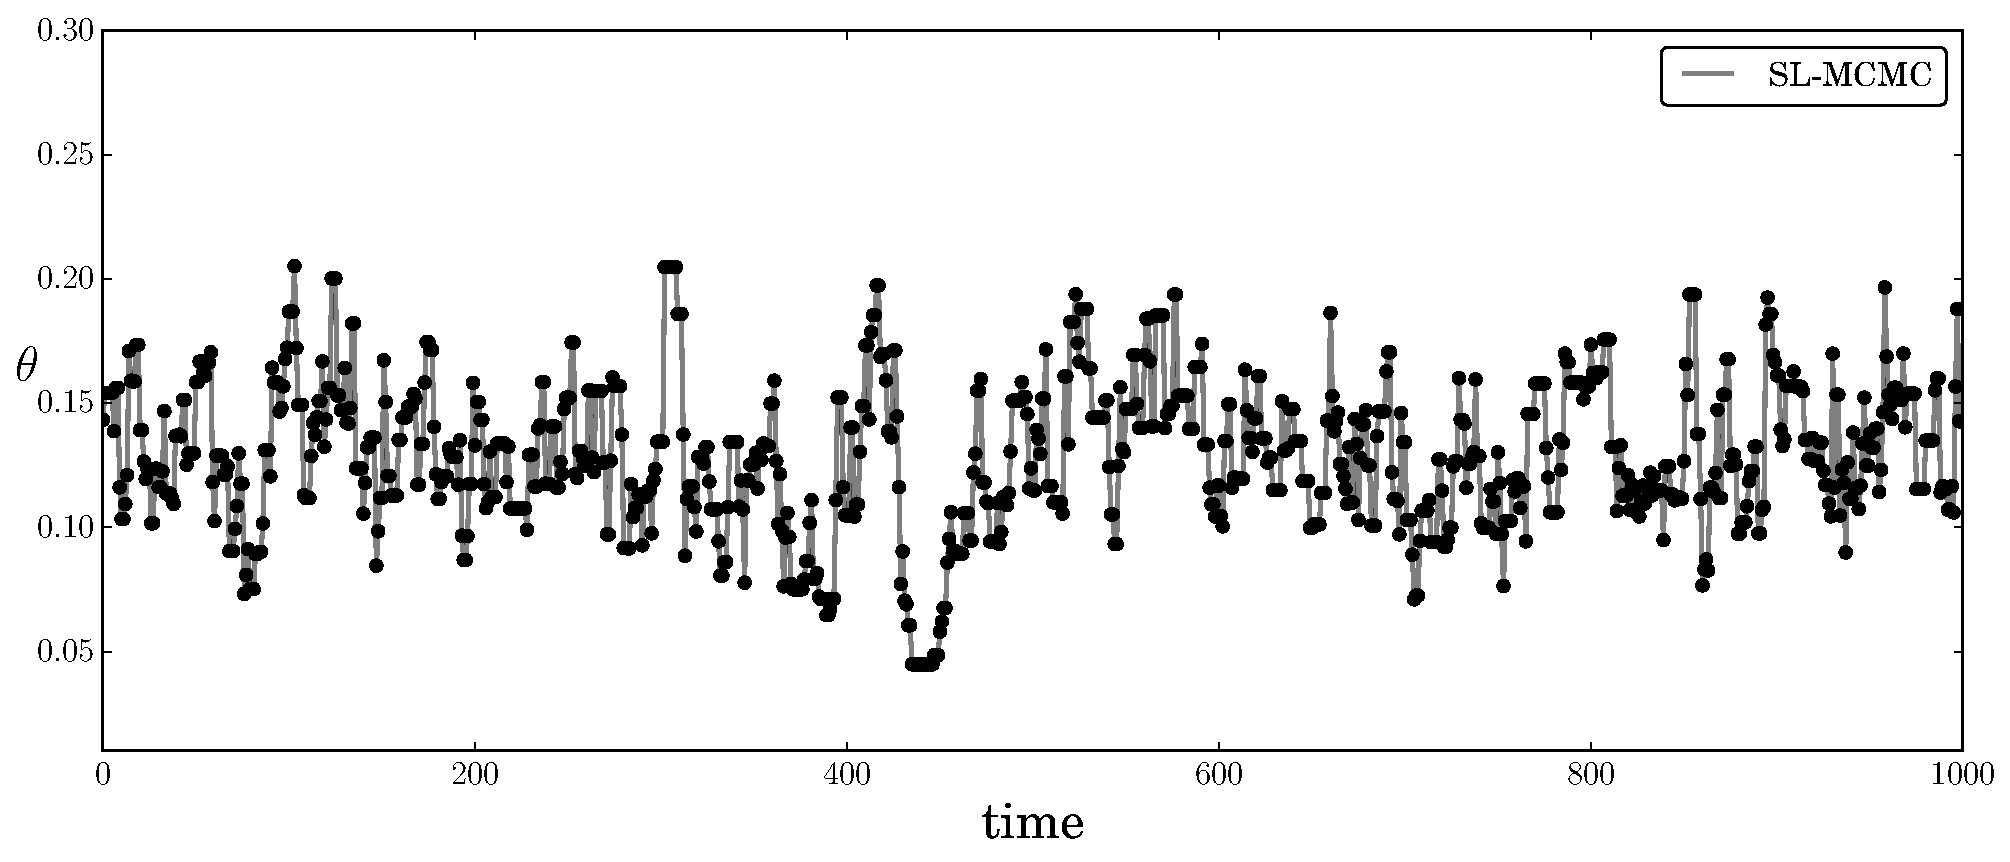
\includegraphics[width=0.95\columnwidth]{./images/exp-SL-MCMC-theta-timeseries-omega-rate-100p0-chain0.pdf}
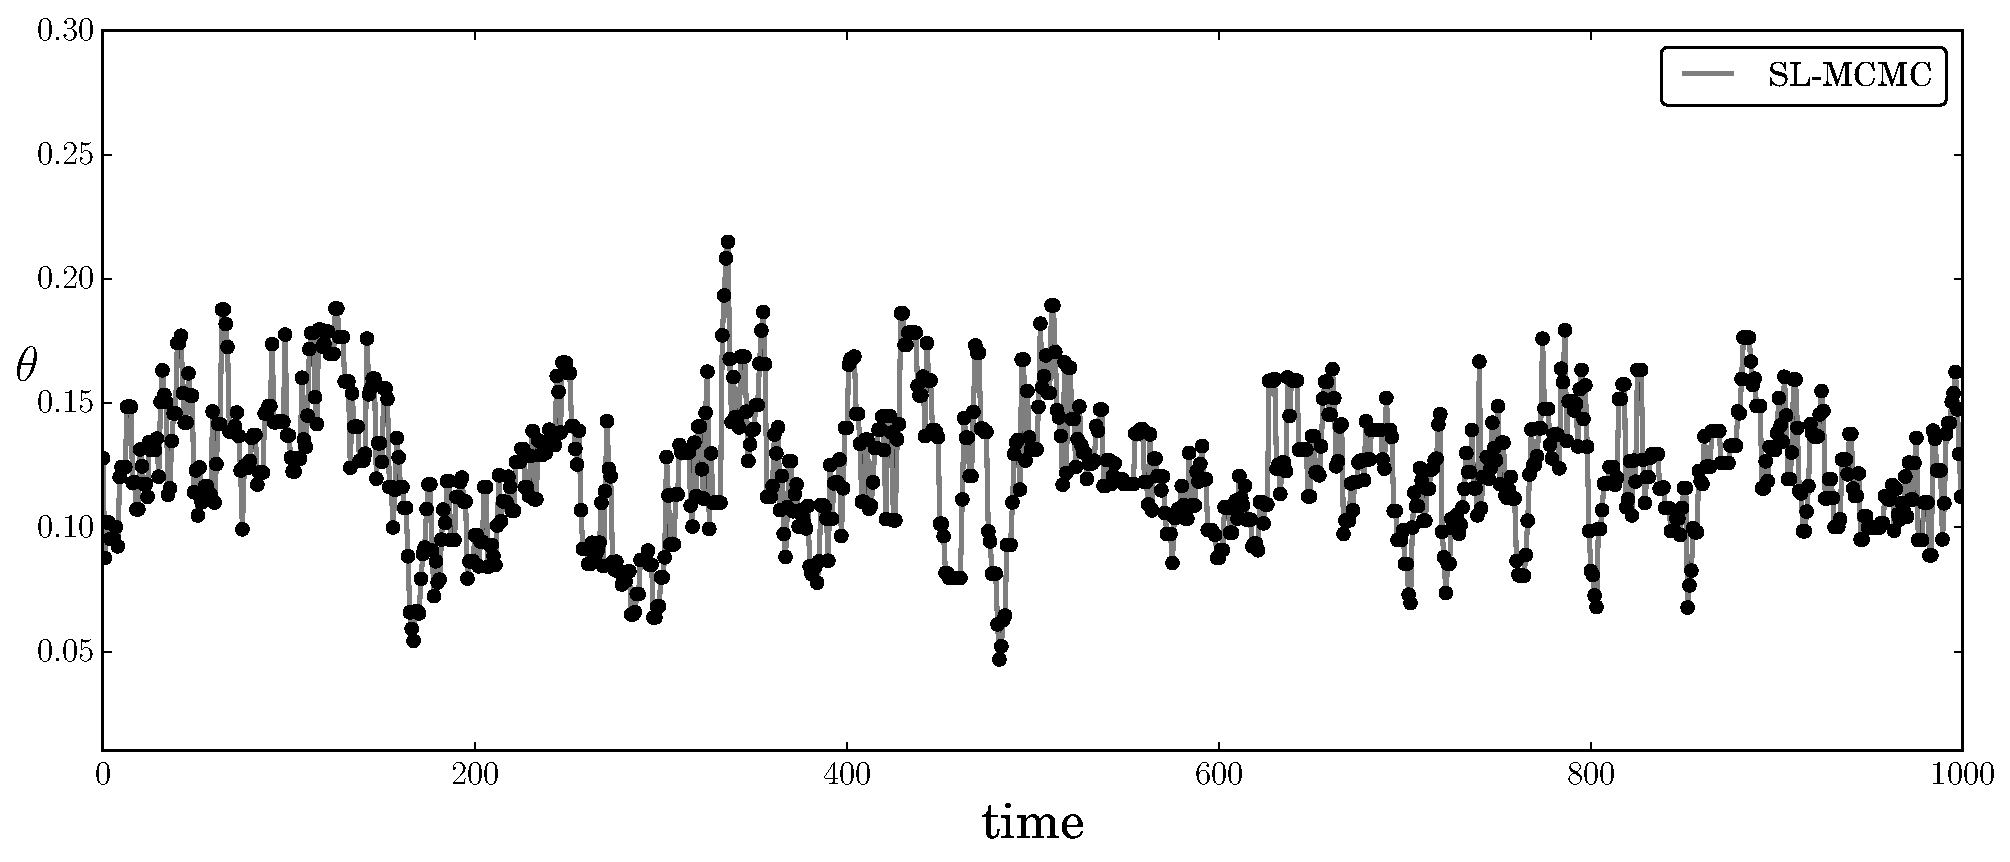
\includegraphics[width=0.95\columnwidth]{./images/exponential/exp2-SL-MCMC-theta-timeseries-omega-rate-0p1-chain3.pdf}
%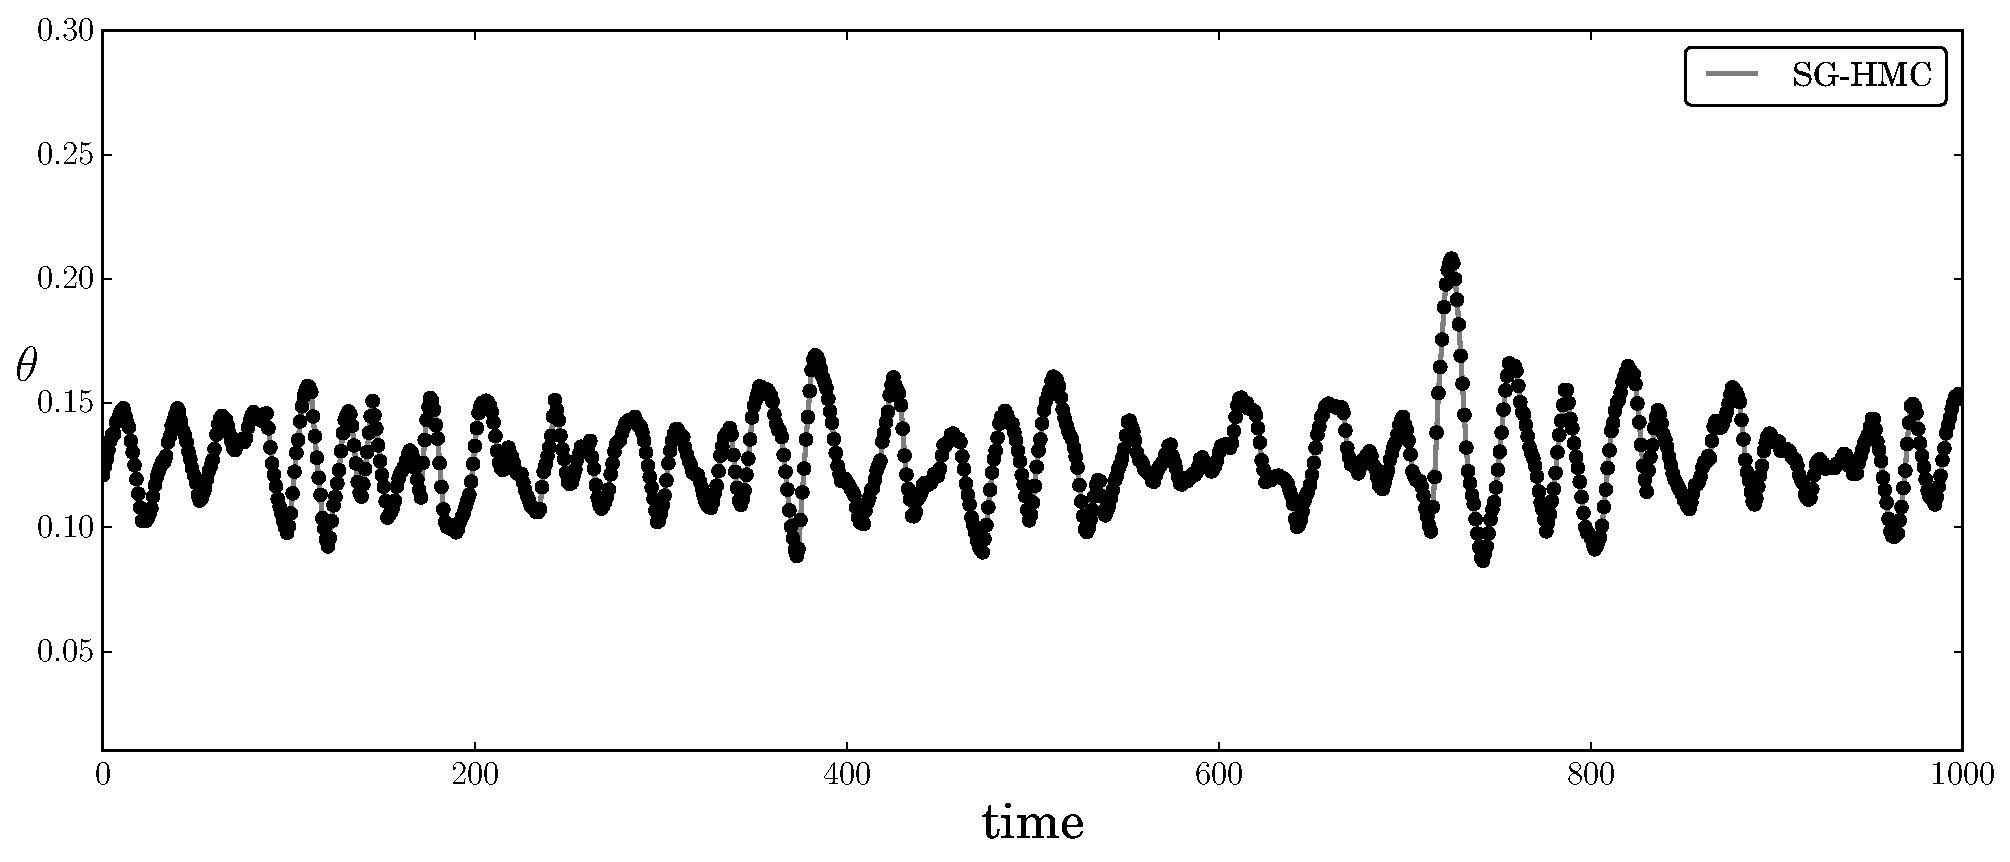
\includegraphics[width=0.95\columnwidth]{./images/exp-SG-HMC-theta-timeseries-omega-rate-100p0-chain0.pdf}
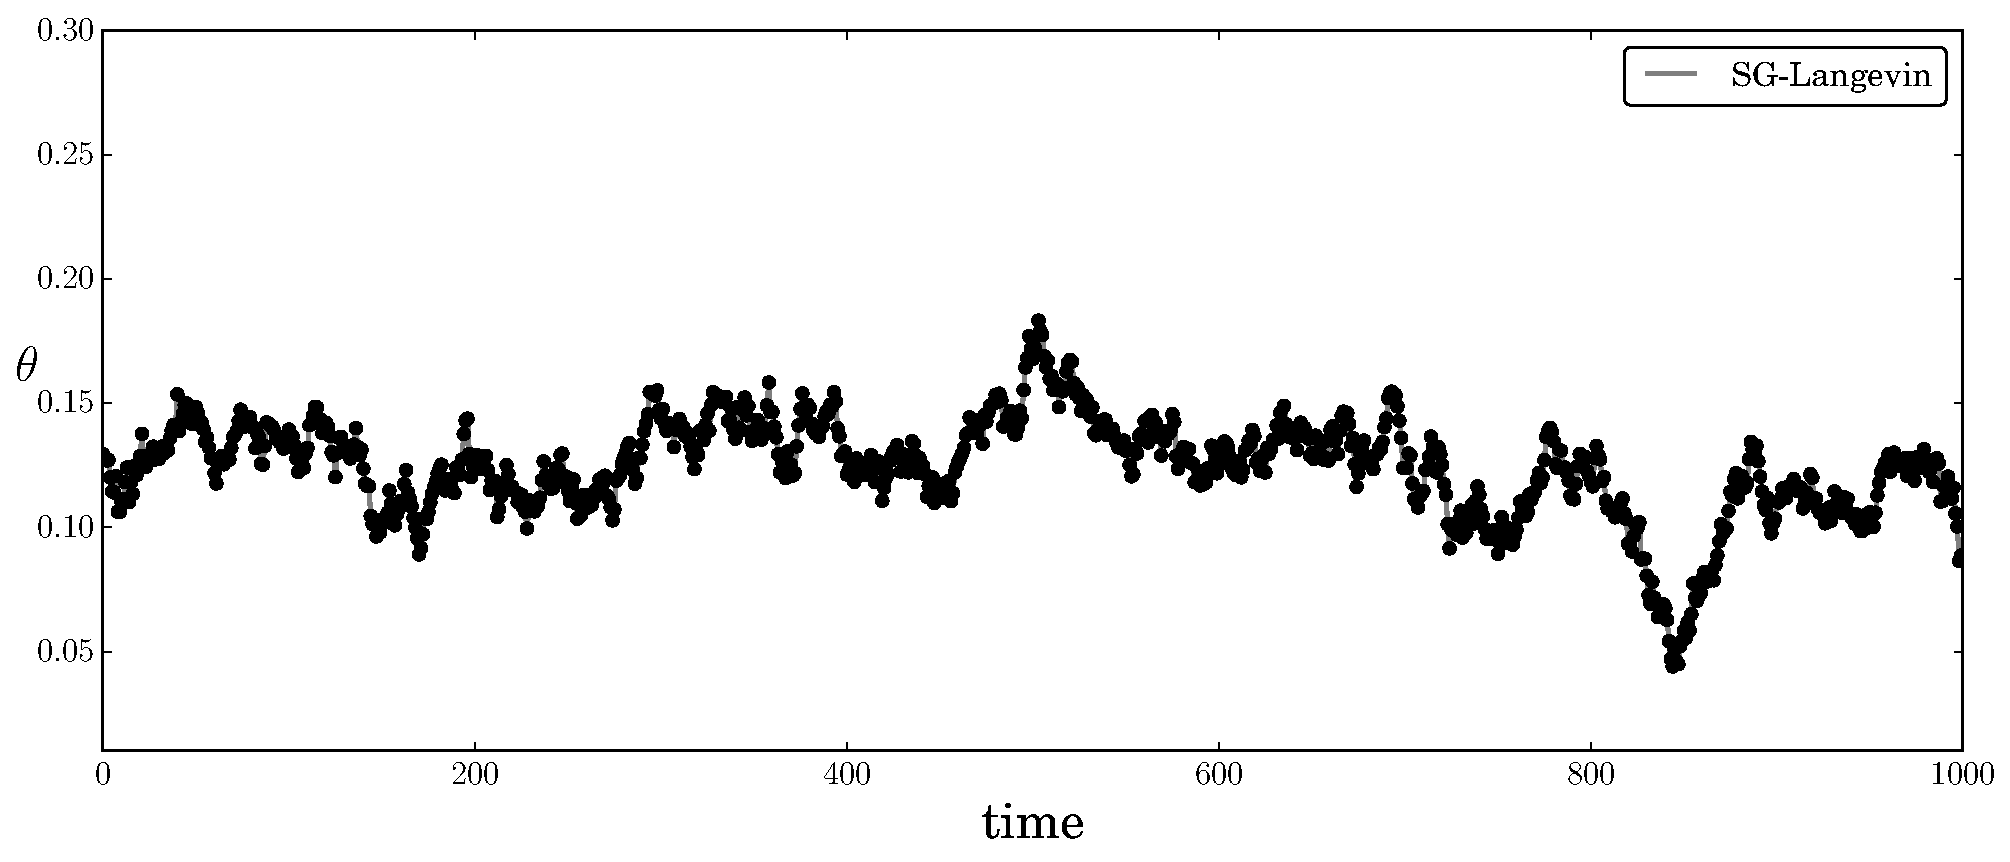
\includegraphics[width=0.95\columnwidth]{./images/exp-SG-Langevin-theta-timeseries-omega-rate-100p0-chain0.pdf}
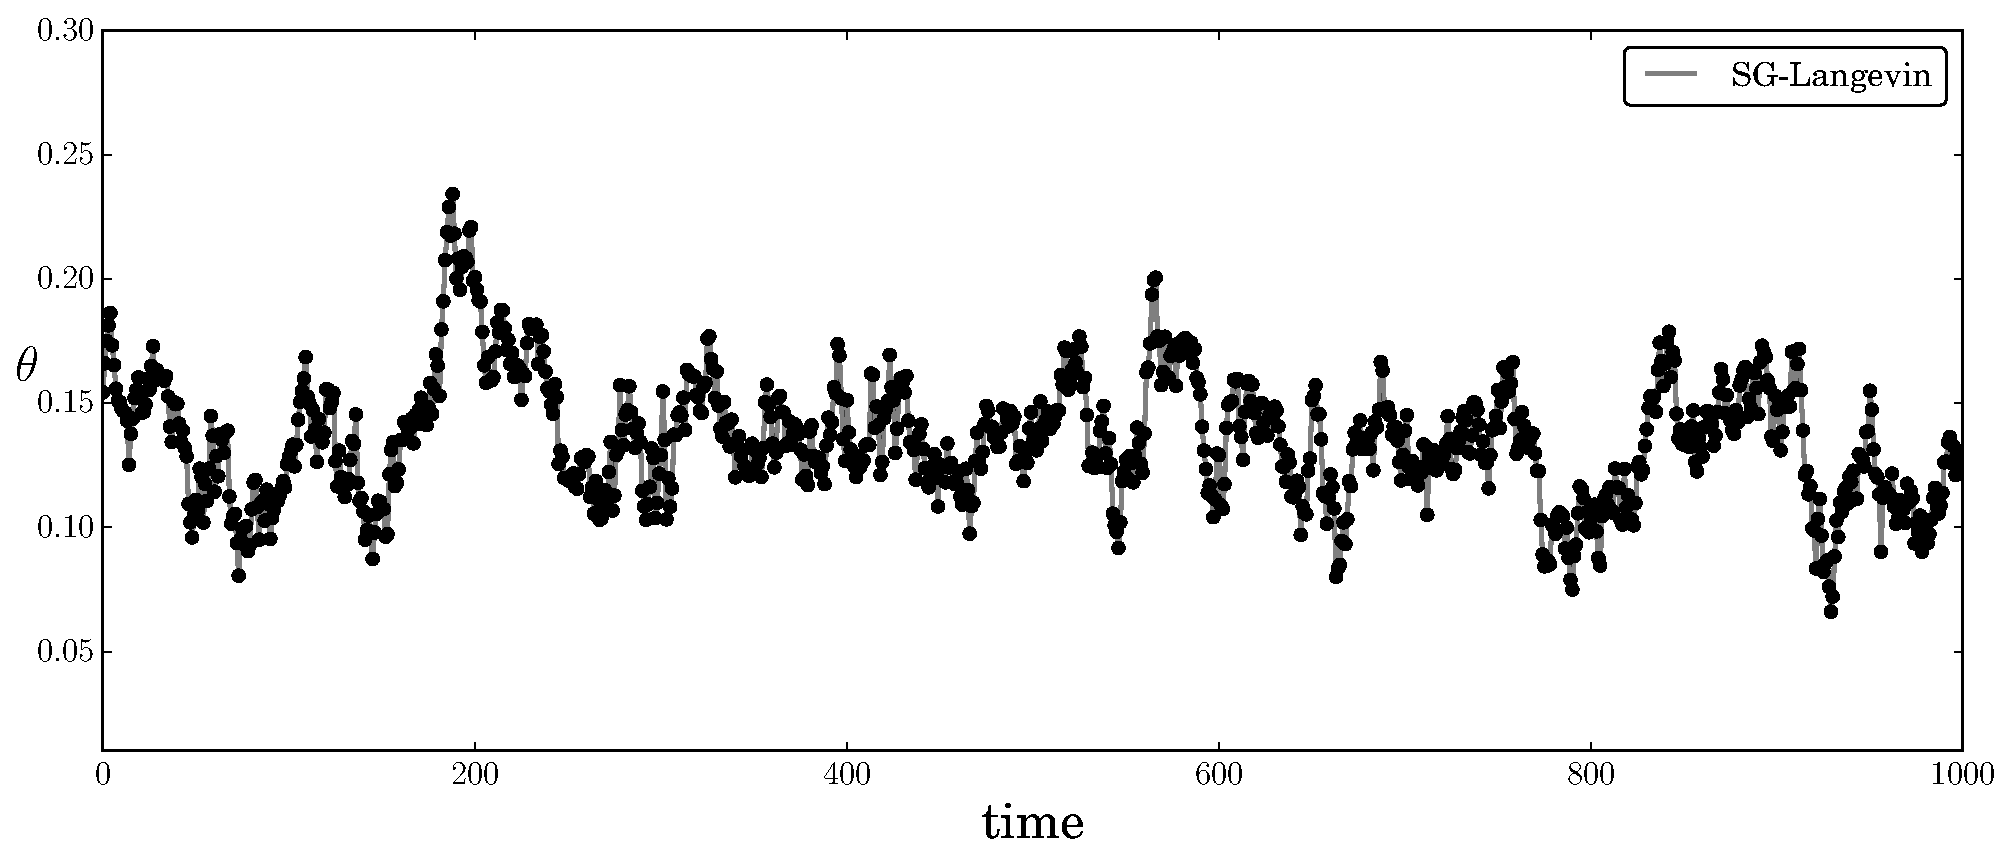
\includegraphics[width=0.95\columnwidth]{./images/exponential/exp2-SG-Langevin-theta-timeseries-omega-rate-0p1-chain3.pdf}
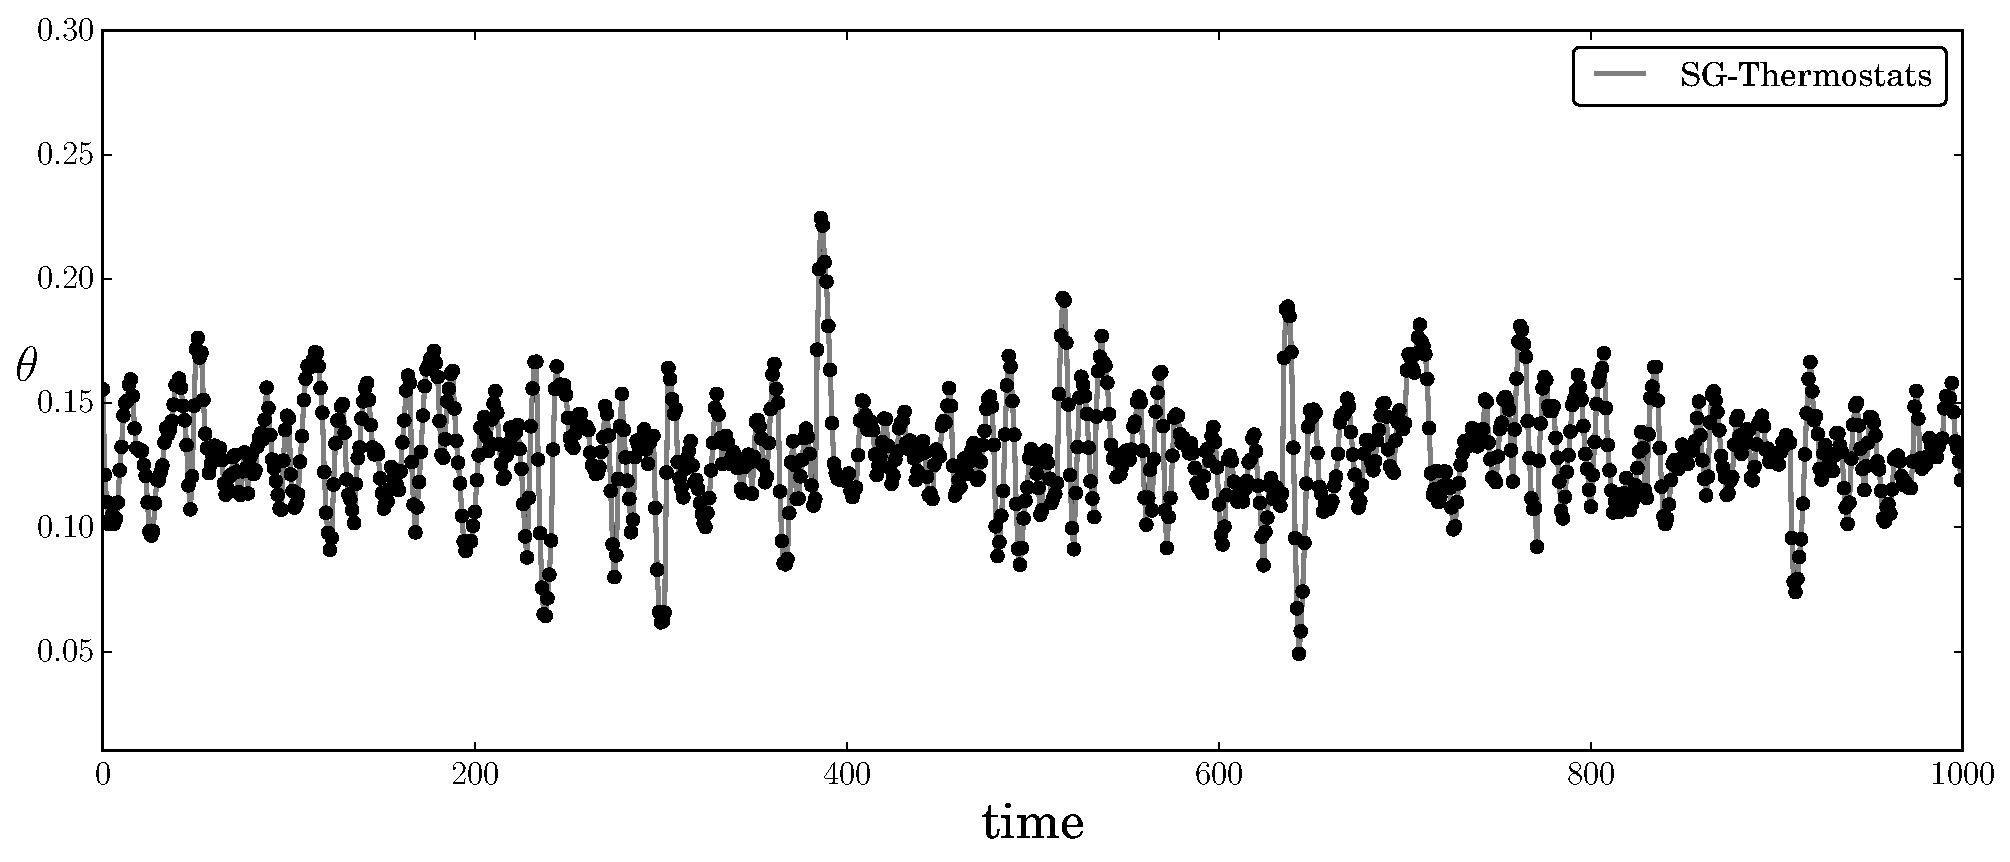
\includegraphics[width=0.95\columnwidth]{./images/exponential/exp3-SG-Thermostats-theta-timeseries-omega-rate-100p0-chain0.pdf}
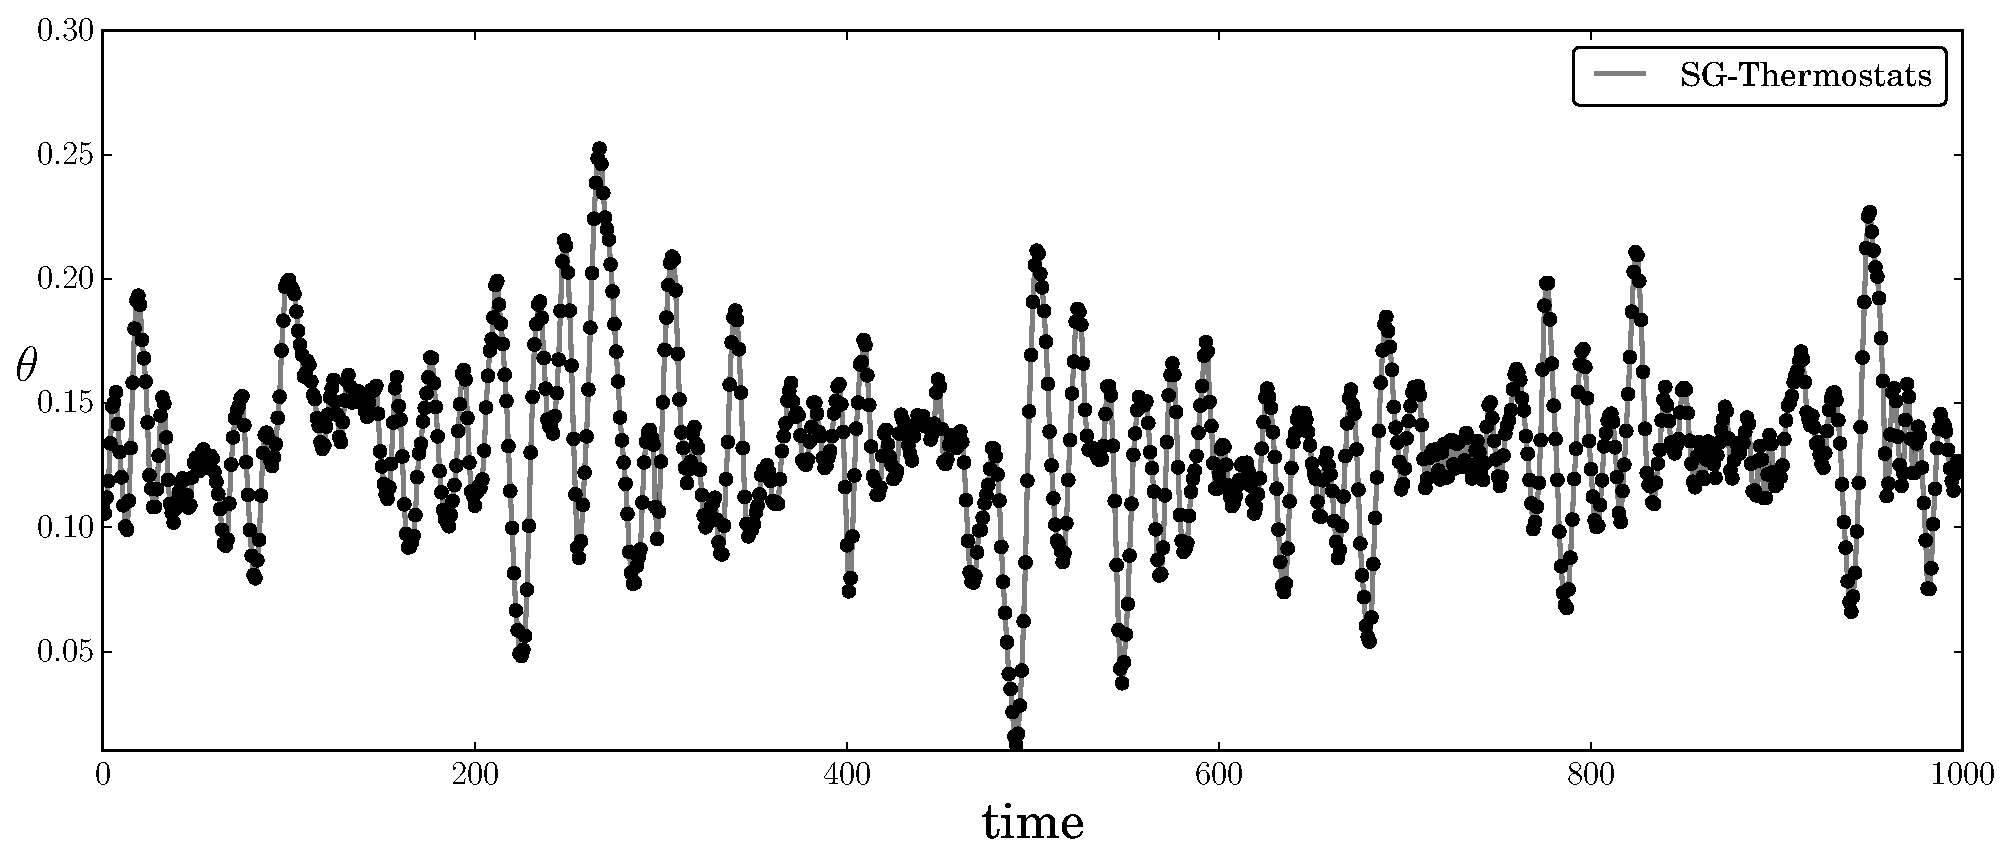
\includegraphics[width=0.95\columnwidth]{./images/exponential/exp2-SG-Thermostats-theta-timeseries-omega-rate-0p1-chain3.pdf}
\caption{\small{Last $1000$ $\thetav$ trajectories for the demonstration problem.  {\bf Left column:} Non-persistent random seeds.  {\bf Right column:} Persistent random seeds with $\gamma = 0.1$.  Each algorithm's parameters were optimized to minimize the total variational distance.  With persistent seeds, each algorithm's random walk behavior is suppressed.  Without persistent seeds, SG-Thermostats chooses a small step-size $\eta$, resulting in an under-dispersed estimate of the posterior; when the seeds are persistent, the gradients are more consistent, allowing for a larger $\eta$ and therefore more injected noise.  The resulting posteriors are shown in Figure~\ref{fig:exp-posteriors}.
%For SG-Thermostats, persistent $\omegav$ allows for larger $\eta$.Sticky  Explanation thermostats: with no %sticky, need to lower eta, so it shows smoother trajectory.  With sticky, the gradients are more consistent, %allowing for a larger eta and therefore more noise injection.
}}
\label{fig:exp-theta-traces}
\end{center}
\vskip -0.2in
\end{figure*}

\subsection{Posterior Inference using HABC}
We ran chains of length $50K$ for SL-MCMC, SGLD, SGHMC, and SGNHT versions of HABC using SL gradient estimates ($S=5$).  A pseudo-marginal version of SL-MCMC was used.  We note that SGHMC gave results nearly identical to SGNHT, so are not shown do to space limitations.   In one set of experiments, common random seeds were used for gradient computations only, and did not persist over time steps; these experiments are called {\em non-persistent}.  In another set of runs, we resampled $\omega_s$ at each time step with probability $\gamma = 0.1$; these experiments are {\em persistent}.  In Figure~\ref{fig:exp-posteriors} we show the posterior distributions for these experiments; in Table~\ref{tab:exp-posterior} we report the {\em total variational distance} between the true posterior and the ABC posteriors using the first $10K$ samples and after $50K$ samples (averaged over $5$ chains).  Of note is the poor approximation of SG-Thermostats when the seeds are not persistent.  By adding persistent seeds, SG-Thermostats gives similar posteriors to the other methods.

In Figure~\ref{fig:exp-theta-traces} we show the trace plots of the last $1000$ samples from a single chain for each algorithm.  In the left column, traces for non-persistent random seeds are shown, and on the right, traces for persistent seeds.  We can observe that persistent random seeds further reduces the random walk behavior of all three methods.  We also observe small improvements in total variational distance for SL-MCMC and SGLD, while SGNHT improves significantly.    
%the random seeds were changed at each time-step In Figure~\ref{fig:exp-theta-traces} we show the posterior trace plots for ABC-MCMC, SGLD, SGHMC, and SGNHT versions of HABC using SL gradient estimates ($S=5$).  The behavior of the trajectories is quite different, though they all produce the same correct posterior estimates (Figure~\ref{fig:exp-posteriors}).  In Table~\ref{tab:exp-posterior} we report the {\em total variational distance} between the true posterior and the ABC posteriors after different numbers of samples (repeated 5 times).

% \begin{table}[h]
% \caption{Posterior inference for Exponential problem}
% \label{tab:exp-prob-no-sticky}
% \begin{center}
% \begin{tabular}{l||c|c|c|c|c}
% {\bf Algo}  & 100 & 1000 & 10K & 50K \\
% \hline \\
% SL-MCMC &  $0.26$ & $0.099$ & $0.047$ & $0.045$ \\
% SGLD    &  $0.42$ & $0.22$ & $0.14$ & $0.045$ \\
% SGHMC   &  $0.26$ & $0.099$ & $0.047$ & $0.045$ \\
% SGNHT   &  $0.26$ & $0.099$ & $0.047$ & $0.045$ \\
% \end{tabular}
% \end{center}
% \end{table}

\begin{table}[h]
\caption{Average total variational distance (tvd) for the demonstration problem.  {\em Non-persistent} used no persistent random seeds, whereas {\em Persistent} randomly proposes a new $\omega_s$ with $\gamma=0.1$. Each algorithms' parameters were optimized for minimal tvd after $10K$ samples.  The results for SGHMC (not shown) and SGNHT are nearly identical.  All algorithms tend to benefit from persistent seeds, in particular SGHMC and SGNHT, the methods with long Hamiltonian trajectories.}
\label{tab:exp-posterior}
\begin{center}
\begin{tabular}{l|c|c||c|c|}
  \cline{2-5}
% Algo & $1000$ & $10000$ & $50000$ \\ \hline \hline
% SL-ABC & $0.099$ & $0.047$ & $0.045$ \\
% SGLD & $0.082$ & $0.049$ & $0.048$ \\
% SGNHT & $0.271$ & $0.162$ & $0.161$ \\
% SGNHT* & $0.144$ & $0.056$ & $0.075$ \\ \hline
 & \multicolumn{2}{|c||}{Non-persistent} & \multicolumn{2}{c|}{Persistent} \\
 \cline{1-5} 
\multicolumn{1}{|l|}{Algo} & $10K$ & $50K$ & $10K$ & $50K$ \\ \hline \hline 
\multicolumn{1}{|l|}{SL-ABC} & $0.047$ & $0.045$ & $0.045$ & $0.045$ \\
\multicolumn{1}{|l|}{SGLD} & $0.049$ & $0.048$ & $0.048$ & $0.043$ \\
%\multicolumn{1}{|l|}{SGHMC} & $0.170$ & $0.165$ & $0.052$ & $0.047$ \\
\multicolumn{1}{|l|}{SGNHT} & $0.232$ & $0.239$ & $0.055$ & $0.051$ \\\hline 
\end{tabular}
\end{center}
\end{table}
% \begin{table}[h]
% \caption{Posterior inference for Exponential problem}
% \label{tab:exp-prob-no-sticky}
% \begin{center}
% \begin{tabular}{l||c|c|c|c|c}
% {\bf Algo}  & 100 & 1000 & 10K & 50K \\
% \hline \\
% SL-MCMC &  $0.23$ & $0.12$ & $0.053$ & $0.044$ \\
% SGLD    &  $0.26$ & $0.099$ & $0.047$ & $0.045$ \\
% SGHMC   &  $0.26$ & $0.099$ & $0.047$ & $0.045$ \\
% SGNHT   &  $0.26$ & $0.099$ & $0.047$ & $0.045$ \\
% \end{tabular}
% \end{center}
% \end{table}

% DIR: exp-eta-0p005-dtheta-0p01-C10-S5-omega-0p01
% SL-MCMC omega_rate 100%
% 
% times 10,   100,  1000,  5000, 10000, 20000, 30000, 40000, 50000
% mean 0.6052864 ,  0.26126289,  0.09895101,  0.05295502,  0.04721529,0.04513989,  0.04622511,  0.04491134,  0.04539522
% std 0.09348374,  0.046628  ,  0.01530586,  0.00861296,  0.00604954, 0.00239858,  0.00327312,  0.00303499,  0.00242383
% 
% omega_Rate 1%
% mean 0.63282705,  0.23141512,  0.11508726,  0.07034678,  0.05338616, 0.05246243,  0.0538948 ,  0.0507813 ,  0.04435618
% std 0.11183616,  0.05139663,  0.05390608,  0.03376141,  0.01785321, 0.0125916 ,  0.00662542,  0.01255384,  0.00603819

% SGLD omega_rate 100%
% array([ 0.66893503,  0.41631787,  0.22451057,  0.15184296,  0.14112572, 0.15204372,  0.14857288,  0.15116372,  0.15076312])
% std(0)array([ 0.08087815,  0.11567097,  0.04555416,  0.03197215,  0.01855117, 0.01417793,  0.01341749,  0.01312386,  0.00855595])
% SGLD omega_rate 1%
% mean 0.75547928,  0.35519016,  0.17736532,  0.09150572,  0.06159863,0.0553024 ,  0.06191501,  0.05637656,  0.05472899
% std 0.11641948,  0.09003194,  0.08414296,  0.03832745,  0.01937652, 0.02211211,  0.01263801,  0.00796597,  0.00836038
% SGHMC omega 100%
% array([ 0.59033585,  0.25581098,  0.24731947,  0.22616621,  0.22842994,
%         0.22780039,  0.22743227,  0.2256994 ,  0.22623605])
%
% In [25]: tvd.std(0)
% Out[25]:
% array([ 0.1870709 ,  0.05443133,  0.04280439,  0.01782881,  0.01695731,
%         0.01044903,  0.00970157,  0.0081758 ,  0.00759141])
% omega 1%
% array([ 0.51193673,  0.36801527,  0.16197407,  0.09853979,  0.0929902 ,
%         0.0976414 ,  0.09743771,  0.09113688,  0.08687801])
%
% In [28]: tvd.std(0)
% Out[28]:
% array([ 0.17030828,  0.10124135,  0.0653025 ,  0.0180961 ,  0.01414473,
%         0.01492984,  0.0169915 ,  0.01351012,  0.009596  ])
% 
% SGTHEMO
% omega 100%
% In [33]: tvd.mean(0)
% Out[33]:
% array([ 0.61253343,  0.2419202 ,  0.15161436,  0.16610309,  0.18284641,
%         0.18875997,  0.19055003,  0.1928232 ,  0.19340706])
%
% In [34]: tvd.std(0)
% Out[34]:
% array([ 0.17654396,  0.04334123,  0.04052037,  0.01846459,  0.0212887 ,
%         0.009026  ,  0.00640309,  0.00575303,  0.00415439])
%

% omega 1%
% In [30]: tvd.std(0)
% Out[30]:
% array([ 0.17343684,  0.10098802,  0.06547166,  0.02232569,  0.01339252,
%         0.01902682,  0.0181153 ,  0.01225494,  0.00760486])
%
% In [31]: tvd.mean(0)
% Out[31]:
% array([ 0.47453793,  0.33112199,  0.14890592,  0.07600464,  0.06685565,
%         0.06371391,  0.06363715,  0.05882387,  0.05590603])




% \subsection{Sticky Random Numbers}
% Finally we compare posterior estimates using sticky CRNs.  Using a flip rate of $1\%$, i.e. each $\omega_s$ has $1\%$ chance of changing randomly at each time-step.  In Figure~\ref{exp-traces-x-sticky} we show the traces plots of $<x^{(s)>}$ for the different methods.  While the Hamiltonian dynamics provide persistence in $\thetav$-space, the sticky random numbers do the same for the ABC statistics.  The Table~\ref{tab:exp-tvd-sticky} we report the same {\em tvd} error using sticky numbers.  [DISCUSS difference with no-sticky]. The potential benefit of using persistent random seeds is shown for all methods, including ABC-MCMC.

%\subsection{Visualizing Noise from Gradient versus Injected Noise}

%%%%%%%%%%%%%%%%%%%%%%%%%%%%%%%%%%%%%%%%%%%%%%%%%
\section{Experiments}\label{sec:experiments}
%%%%%%%%%%%%%%%%%%%%%%%%%%%%%%%%%%%%%%%%%%%%%%%%%
We present experimental results comparing HABC with standard ABC-MCMC for two challenging simulators.  The first is low-dimensional ($D=6$), but exhibits chaotic behavior.  For the second problem we apply the techniques of HABC to a Bayesian image classifier and autoencoder.  The benefit of this problem is we can compare directly with the SGHD algorithms using the analytic gradients.  This problem is has very high-dimension ($D>15000$), yet we are able to successfully apply SPSA-based gradients to HABC. 


\subsection{Blowfly}\label{sec:bf}
For these experiments, a simulator of adult sheep blowfly populations \cite{wood2010statistical} is used with statistics set to those from \cite{Meeds2014GpsUai}.  The observational vector $\y$ is a time-series of a fly population counted daily. The population dynamics are modeled using a stochastic differential equation\footnote{Equation~1 in Section 1.2.3 of the supplementary information in \cite{wood2010statistical}.}
\begin{equation}
N_{t+1} = P N_{t-\tau} \exp(-N_{t-\tau}/N_0) e_t + N_t \exp(-\delta \epsilon_t) \nonumber
\end{equation}
where $e_t \sim  \mathcal{G}( 1/{\sigma_p^2},1/{\sigma_p^2})$ and $\epsilon_t 
 \sim  \mathcal{G}( 1/{\sigma_d^2},1/{\sigma_d^2})$  
are sources of noise, and $\tau$ is an integer.  In total, there are $D=6$ parameters $\theta = \{ \log P, \log \delta, \log N_0, \log \sigma_d, \log \sigma_p, \tau\}$.  As \cite{Meeds2014GpsUai} we place broad log-normal priors over $\theta_{1\ldots 5}$ and a Poisson prior over $\tau$.  This is considered a challenging problem because slight changes to some parameter settings can produce degenerate $\x$, while others settings can be very noisy due to the chaotic nature of the equations.  The statistics from \cite{Meeds2014GpsUai} are used ($J=10$): the log average of $4$ quantiles of $N/1000$, the average of $4$ quantiles of the first-order differences in $N/1000$, and the number of maximal population peaks under two different thresholds. 

%\subsubsection{Posterior Inference using HABC}
We compare difference HABC algorithms with ABC-MCMC for the blowfly population problem.  We use $\epsvec = \{ 1/2,1/2,1/2,1/2, 1/4,1/4,1/4,1/4,3/4,3/4 \}$ (slightly different $\epsvec$ from \cite{Meeds2014GpsUai}) and $S=10$ for all experiments.  We use SPSA with $R=1$ using SL log-likelihoods for all HABC gradient estimates.  Note that this requires $2S$ forward simulations per time-step, the same as marginal ABC and twice pseudo-marginal ABC.  

Figure~\ref{fig:bf-posterior-histograms} show the posterior distributions for $\log P, \log \delta$ and the posterior predictive distributions of [FILL IN].  Traces of $\thetav$ are shown for SGHMC and SGNHT in Figure~\ref{}.  Finally, we compare the convergence to $\y$ using the online posterior predictive distribution in Figure~\ref{}.  By using stick random numbers, the convergence is [FILL IN].
  
\begin{figure}[t]
\vskip 0.2in
\begin{center}
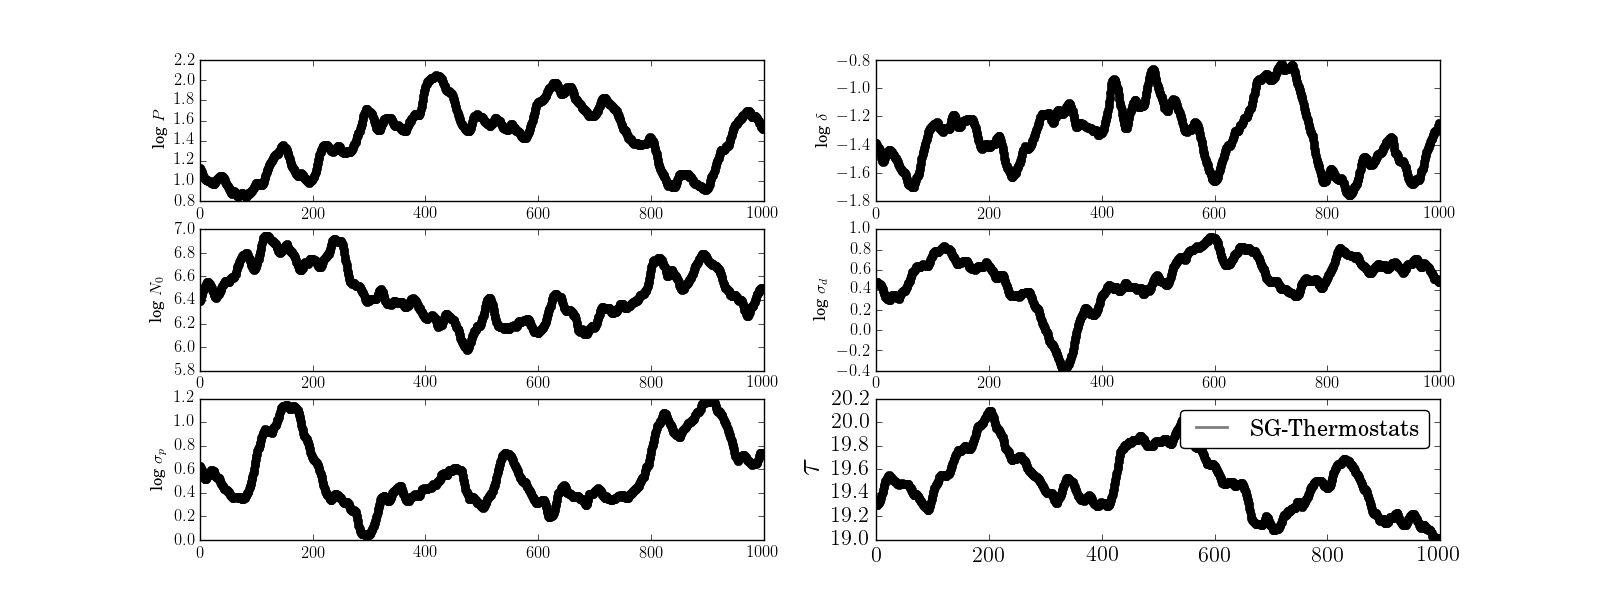
\includegraphics[width=1.1\columnwidth]{./images/blowfly/bf_theta_thermo_timeseries.png}
%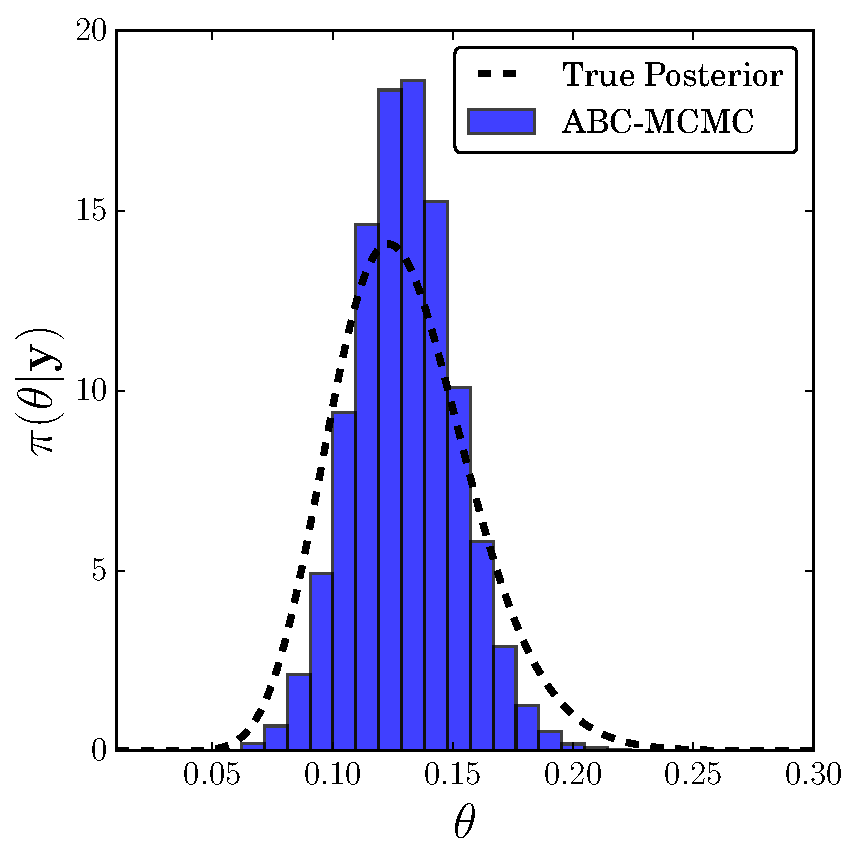
\includegraphics[width=0.45\columnwidth]{./images/exp-ABC-MCMC-posterior_hist.pdf}
%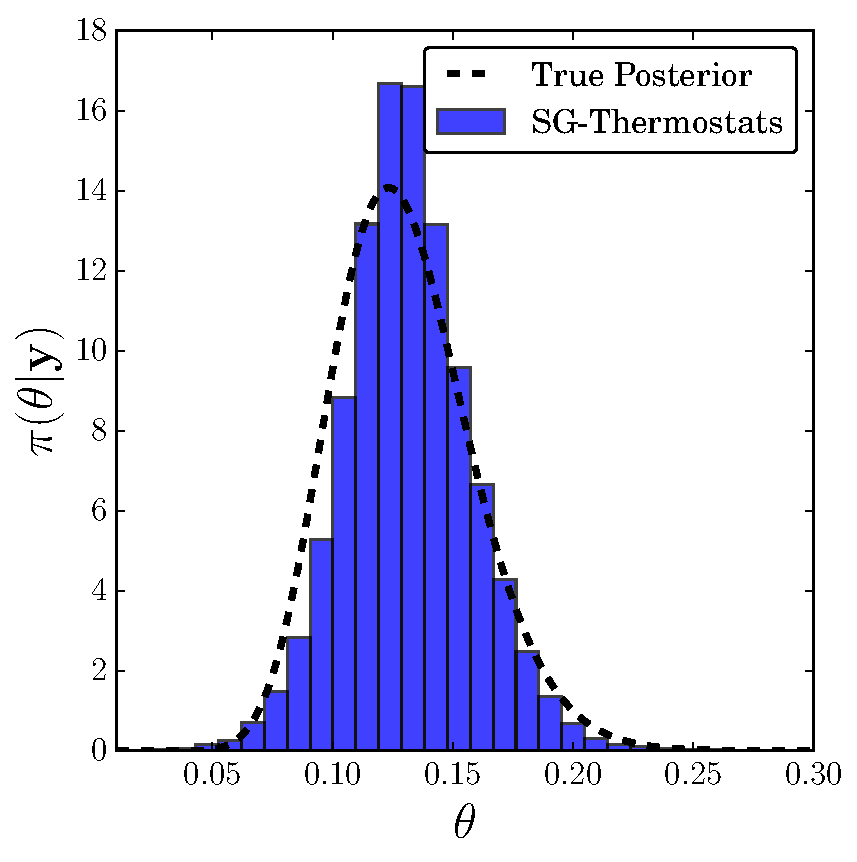
\includegraphics[width=0.45\columnwidth]{./images/exp-SG-Thermostats-posterior_hist.pdf}
%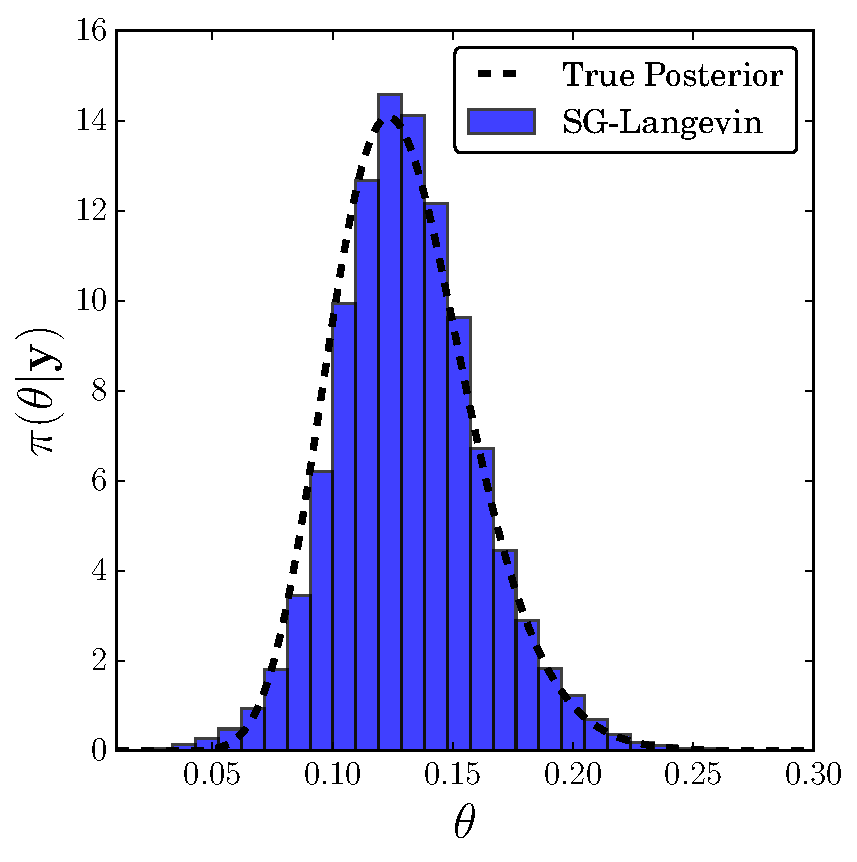
\includegraphics[width=0.45\columnwidth]{./images/exp-SG-Langevin-posterior_hist.pdf}
%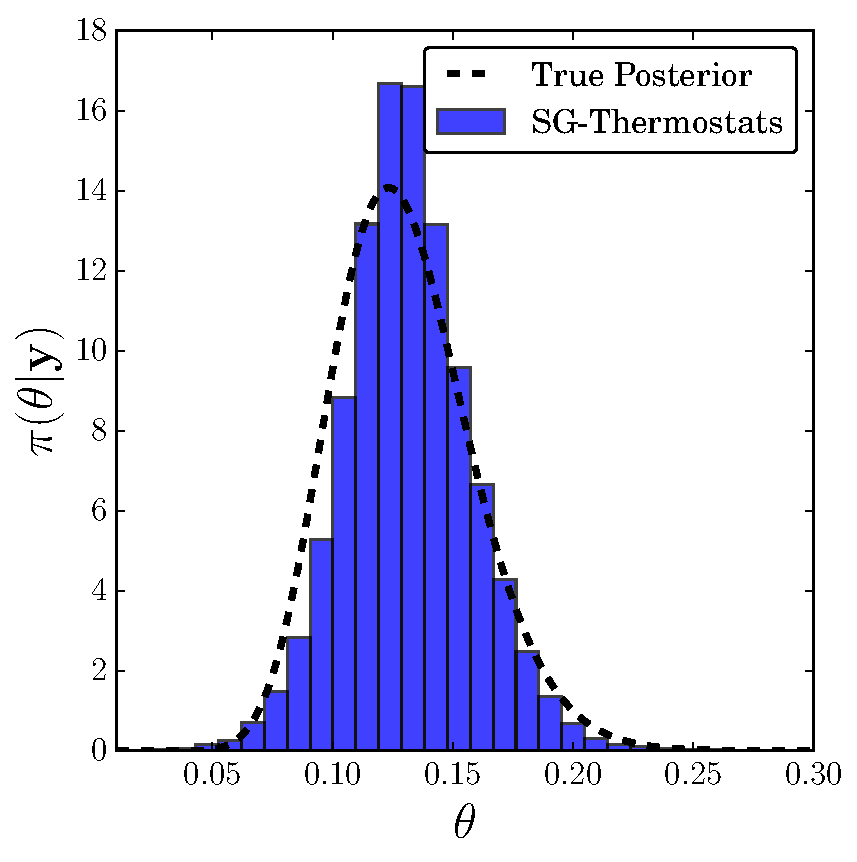
\includegraphics[width=0.45\columnwidth]{./images/exp-SG-Thermostats-posterior_hist.pdf}
\caption{\small{}}
\label{fig:exp-posteriors}
\end{center}
\vskip -0.2in
\end{figure} 



\subsection{Bayesian Autoencoders}\label{sec:auto}
We perform Bayesian inference on an autoencoder neural network using MNIST images as observations.  We apply two inference algorithms: SGNHT and HABC.  For SGNHT, we use the known gradient and for HABC we apply 2SPSA.  After 1000 iterations we collect parameter vectors every 100 iterations for a total of 100 sets. (Do we use SGHMC to estimate Bhat in first 1000 iterations?).  Use same batches at each iteration for SGNHT and HABC? 

results: convergence of training error (batches), convergence in test error using parameters collected (record nbr of forward or backward passes required), show mean and variance of filters (how?), compare with using the last parameter sample only (stochastic optimization).





%%%%%%%%%%%%%%%%%%%%%%%%%%%%%%%%%%%%%%%%%%%%%%%%%
%\section{DISCUSSION} \label{sec:discussion}
%%%%%%%%%%%%%%%%%%%%%%%%%%%%%%%%%%%%%%%%%%%%%%%%%

% \begin{itemize}
%   \item
%   \item
% \end{itemize}

%%%%%%%%%%%%%%%%%%%%%%%%%%%%%%%%%%%%%%%%%%%%%%%%%
\section{DISCUSSION AND CONCLUSION} \label{sec:conclusion}
%%%%%%%%%%%%%%%%%%%%%%%%%%%%%%%%%%%%%%%%%%%%%%%%%
Hamiltonian ABC proposes a new set of algorithms for Bayesian inference of likelihood-free models.  HABC builds  upon the connections between Hamilton Monte Carlo with stochastic gradients and well-established gradient approximations based on a minimal number of forward simulations, even for high-dimensional parameter spaces.  By showing the feasibility of running ABC in high-dimensions, we hope that the door has been opened for exploration of larger simulation-based models. 

Another innovation we introduce is the use of sticky or persistent random seeds to suppress the simulator noise and therefore smooth the simulation landscape over a local region of parameter space.  By doing this, all our methods, but especially SGHMC and SGNHT, with their longer Hamiltonian trajectories, benefit from this smoothness that changes slowly over time.  We feel that new classes of ABC algorithms could develop from using persistent random seeds, not solely gradient-based samplers.
 
There are several unresolved and open questions regarding the application of stochastic gradients to ABC.  The first issue is the importance of the bias-variance relationship for different ABC likelihood models.    We found that using gradients based on the synthetic-likelihood greatly reduced their variance, but introduced a small bias, because of its Gaussian assumption.  The second issue is setting algorithm parameters, in particular the step-sizes $\eta$, the injected noise $C$ (for SGHMC/SGNHT), and the number of SPSA repetitions $R$.  All of these parameters are highly interactive.  Can we use statistical tests during the MCMC run to determine $R$?  Are should $\eta$ and $C$ be set differently in the ABC setting?  One final issue is monitoring or determining whether the correct amount of noise is being injected to ensure proper sampling.  In SGLD, for example, we can always turn down $\eta$ so that the injected noise term dominates, but when our goal is efficient exploration of the posterior, this is a not very satisfying solution.

% \begin{itemize}
%   \item New set of ABC algorithms for efficient exploration of posterior distribution.
%   \item Key: opens the door to high-dimensional ABC inference.
%   \item [Test for more accurate gradients] For ABC, the gradients we compute are stochastic because we must approximate $\pi(\x | \thetav)$ with forward simulations.  We can make the approximation arbitrarily good by running more simulations, but this is often unnecessary for sampling, because we can make use of the uncertainty in our current approximation to decide if our sample is correct or not (cite UAI2014?).
%   \item Unbiased gradients with low noise.  SL bias might be intolerable; use KDE to get stable unbiased gradients?
% \end{itemize}

Expensive simulators are an important class of models that we do not address in this work.  However, previous work in Bayesian inference has shown the usefulness of HMC-based proposals based on Gaussian process of log-likelihood surfaces \cite{rasmussen:2003}.   We could similarly use HABC with recent ABC surrogate models \cite{Meeds2014GpsUai,wilkinson:2014} to avoid simulations whenever possible, yet benefit from Hamiltonian dynamics.  
%We address this scenario in Section~\ref{future}.  
%Shown for relatively fast simulators.  Extensions to surrogates with GPS (Meeds2014GpsUai, rasmussen:2003, wilkinson:2014) can use derivative of GP for likelihood as GP of gradient.  These could be matched by occasional gradient estimates (Osborne).

%\subsubsection*{References}
%{
\clearpage
\bibliographystyle{icml2014}
\bibliography{abcsgld}
%}

\end{document}